\documentclass{article}

% Recommended, but optional, packages for figures and better typesetting:
\usepackage{microtype}
\usepackage{graphicx}
\usepackage{subfigure}
\usepackage{caption}
\usepackage{booktabs} % for professional tables
\usepackage{multirow}
\usepackage{pythonhighlight}
%\usepackage{placeins}

% hyperref makes hyperlinks in the resulting PDF.
% If your build breaks (sometimes temporarily if a hyperlink spans a page)
% please comment out the following usepackage line and replace
% \usepackage{icml2025} with \usepackage[nohyperref]{icml2025} above.
\usepackage{hyperref}


% Attempt to make hyperref and algorithmic work together better:
\newcommand{\theHalgorithm}{\arabic{algorithm}}

% Use the following line for the initial blind version submitted for review:
%\usepackage{icml2025}

% If accepted, instead use the following line for the camera-ready submission:
\usepackage[accepted]{icml2025}

% For theorems and such
\usepackage{amsmath,bm}
\usepackage{amssymb}
\usepackage{mathtools}
\usepackage{amsthm}

% if you use cleveref..
\usepackage[capitalize,noabbrev]{cleveref}

%%%%%%%%%%%%%%%%%%%%%%%%%%%%%%%%
% THEOREMS
%%%%%%%%%%%%%%%%%%%%%%%%%%%%%%%%
\theoremstyle{plain}
\newtheorem{theorem}{Theorem}[section]
\newtheorem{proposition}[theorem]{Proposition}
\newtheorem{lemma}[theorem]{Lemma}
\newtheorem{corollary}[theorem]{Corollary}
\theoremstyle{definition}
\newtheorem{definition}[theorem]{Definition}
\newtheorem{assumption}[theorem]{Assumption}
\theoremstyle{remark}
\newtheorem{remark}[theorem]{Remark}

%%%%%%%%%%%%%%%%%%%%%%%%%%%%%%%%
% Vectors & Matrices
%%%%%%%%%%%%%%%%%%%%%%%%%%%%%%%%
\newcommand{\va}{\mathbf{a}}
\newcommand{\vb}{\mathbf{b}}
\newcommand{\vc}{\mathbf{c}}
\newcommand{\vd}{\mathbf{d}}
\newcommand{\ve}{\mathbf{e}}
\newcommand{\vf}{\mathbf{f}}
\newcommand{\vg}{\mathbf{g}}
\newcommand{\vh}{\mathbf{h}}
\newcommand{\vi}{\mathbf{i}}
\newcommand{\vj}{\mathbf{j}}
\newcommand{\vk}{\mathbf{k}}
\newcommand{\vl}{\mathbf{l}}
\newcommand{\vm}{\mathbf{m}}
\newcommand{\vn}{\mathbf{n}}
\newcommand{\vo}{\mathbf{o}}
\newcommand{\vp}{\mathbf{p}}
\newcommand{\vq}{\mathbf{q}}
\newcommand{\vr}{\mathbf{r}}
\newcommand{\vs}{\mathbf{s}}
\newcommand{\vt}{\mathbf{t}}
\newcommand{\vu}{\mathbf{u}}
\newcommand{\vv}{\mathbf{v}}
\newcommand{\vw}{\mathbf{w}}
\newcommand{\vx}{\mathbf{x}}
\newcommand{\vy}{\mathbf{y}}
\newcommand{\vz}{\mathbf{z}}
\newcommand{\vA}{\mathbf{A}}
\newcommand{\vB}{\mathbf{B}}
\newcommand{\vC}{\mathbf{C}}
\newcommand{\vD}{\mathbf{D}}
\newcommand{\vE}{\mathbf{E}}
\newcommand{\vF}{\mathbf{F}}
\newcommand{\vG}{\mathbf{G}}
\newcommand{\vH}{\mathbf{H}}
\newcommand{\vI}{\mathbf{I}}
\newcommand{\vJ}{\mathbf{J}}
\newcommand{\vK}{\mathbf{K}}
\newcommand{\vL}{\mathbf{L}}
\newcommand{\vM}{\mathbf{M}}
\newcommand{\vN}{\mathbf{N}}
\newcommand{\vO}{\mathbf{O}}
\newcommand{\vP}{\mathbf{P}}
\newcommand{\vQ}{\mathbf{Q}}
\newcommand{\vR}{\mathbf{R}}
\newcommand{\vS}{\mathbf{S}}
\newcommand{\vT}{\mathbf{T}}
\newcommand{\vU}{\mathbf{U}}
\newcommand{\vV}{\mathbf{V}}
\newcommand{\vW}{\mathbf{W}}
\newcommand{\vX}{\mathbf{X}}
\newcommand{\vY}{\mathbf{Y}}
\newcommand{\vZ}{\mathbf{Z}}
\newcommand{\vtheta}{\bm{\theta}}
\newcommand{\veps}{\bm{\varepsilon}}
\newcommand{\pd}[2]{\frac{\partial{#1}}{\partial{#2}}}

% Todonotes is useful during development; simply uncomment the next line
%    and comment out the line below the next line to turn off comments
%\usepackage[disable,textsize=tiny]{todonotes}
\usepackage[textsize=tiny]{todonotes}

\usepackage{pgfplots}
\usepackage{tikz-cd}
\usepackage{wrapfig}
\usepackage{subcaption}
\usepackage{stfloats}
%\usepackage{fixltx2e}
%\usepackage{dblfloatfix}
%\usepackage{nidanfloat}

% The \icmltitle you define below is probably too long as a header.
% Therefore, a short form for the running title is supplied here:
\icmltitlerunning{Enforcing idempotency in neural networks}

\begin{document}

\twocolumn[
    \icmltitle{Enforcing idempotency in neural networks}

    % It is OKAY to include author information, even for blind
    % submissions: the style file will automatically remove it for you
    % unless you've provided the [accepted] option to the icml2025
    % package.

    % List of affiliations: The first argument should be a (short)
    % identifier you will use later to specify author affiliations
    % Academic affiliations should list Department, University, City, Region, Country
    % Industry affiliations should list Company, City, Region, Country

    % You can specify symbols, otherwise they are numbered in order.
    % Ideally, you should not use this facility. Affiliations will be numbered
    % in order of appearance and this is the preferred way.
    \icmlsetsymbol{equal}{*}

    \begin{icmlauthorlist}
        \icmlauthor{Nikolaj Banke Jensen}{equal,ox}
        \icmlauthor{Jamie Vicary}{equal,cam}
    \end{icmlauthorlist}

    \icmlaffiliation{ox}{Department of Computer Science, University of Oxford, Oxford, England}
    \icmlaffiliation{cam}{Department of Computer Science and Technology, University of Cambridge, Cambridge, England}

    \icmlcorrespondingauthor{Nikolaj Banke Jensen}{nikolaj.jensen@cs.ox.ac.uk}
    \icmlcorrespondingauthor{Jamie Vicary}{jamie.vicary@cl.cam.ac.uk}

    % You may provide any keywords that you
    % find helpful for describing your paper; these are used to populate
    % the "keywords" metadata in the PDF but will not be shown in the document
    \icmlkeywords{idempotent neural networks, non-convex optimization, gradient-free optimization, machine learning, ICML}

    \vskip 0.3in
]

% this must go after the closing bracket ] following \twocolumn[ ...

% This command actually creates the footnote in the first column
% listing the affiliations and the copyright notice.
% The command takes one argument, which is text to display at the start of the footnote.
% The \icmlEqualContribution command is standard text for equal contribution.
% Remove it (just {}) if you do not need this facility.

%\printAffiliationsAndNotice{}  % leave blank if no need to mention equal contribution
\printAffiliationsAndNotice{\icmlEqualContribution} % otherwise use the standard text.

\begin{abstract}
    In this work, we propose a new architecture-agnostic method for training idempotent neural networks. An idempotent operator satisfies $f(x) = f(f(x))$, meaning it can be applied iteratively with no effect beyond the first application. Some neural networks used in data transformation tasks, such as image generation and augmentation, can represent non-linear idempotent projections. Using methods from perturbation theory we derive the recurrence relation ${\mathbf{K}' \leftarrow 3\mathbf{K}^2 - 2\mathbf{K}^3}$ for iteratively projecting a real-valued matrix $\mathbf{K}$ onto the manifold of idempotent matrices. Our analysis shows that for linear, single-layer MLP networks this projection 1) has idempotent fixed points, and 2) is attracting only around idempotent points. We give an extension to non-linear networks by considering our approach as a substitution of the gradient for the canonical loss function, achieving an architecture-agnostic training scheme. We provide experimental results for MLP- and CNN-based architectures with significant improvement in idempotent error over the canonical gradient-based approach. Finally, we demonstrate practical applications of the method as we train a generative network successfully using only a simple reconstruction loss paired with our method.
\end{abstract}

% (1 page)
\section{Introduction}
\label{sec:intro}
% \textit{Introduce the idea of idempotent neural networks; give the definition. Justification for usefulness in applications where solutions can be both idempotent and not, and where the idempotent solution may be beneficial. Give a brief overview of the rest of the paper.}

% Wider context -> Idempotent networks
Using neural networks as data augmentation tools is becoming more widespread in areas such as signal processing and generative artificial intelligence. In particular, networks of the form ${f: X \to X}$, mapping data within the same space $X$, are frequently used in image augmentation \cite{lu-image-aug}, video generation \cite{ma-compression, liu-gans}, sorting algorithms \cite{tambouratzis-sorting}, compression algorithms \cite{namphol-compression, liu-gans}, image denoising \cite{mao-deblurring, ilesanmi-denoising, liu-gans}, and image generation \cite{liu-gans}, among others.

Some data transformation tasks admit \textit{only} idempotent solutions (\textit{e.g.}, sorting), whilst other tasks admit \textit{no} idempotent solutions (\textit{e.g.}, rotating an image by 90$^{\circ}$). This work is concerned with a class of data transformation tasks which has both idempotent and non-idempotent solutions and where idempotency might be a desirable property. For example, in Section \ref{sec:experiment} we study idempotency in generative networks where it is the formal requirement of one-step inference, but also denoising and image augmentation (\textit{e.g.}, application of effect-filters) are examples of tasks where idempotent solutions may be desirable \cite{mao-deblurring,liu-gans}. Since solutions are not intrinsically idempotent in this class, we explore actively enforcing idempotency as a component of the loss function used in training.

%While there is a variety of such transformation tasks, some of these can be considered \textit{intrinsically idempotent} in the sense that any function which carries out the transformation is necessarily an idempotent operator. An idempotent operation is one which can be applied iteratively with no effect beyond the first application. For instance, a sorting transformation is intrinsically idempotent since sorting an already sorted data structure is redundant and such a sorting is often deterministic. On the other hand, image transformations might not always be idempotent: rotating an image by 90$^{\circ}$ twice is not the same as rotating it once, for instance. As such, some transformations are intrinsically idempotent and admit \textit{only} idempotent solutions while other tasks are not and admit \textit{no} idempotent solutions. This work, however, is concerned with a class of data transformation tasks which has both idempotent and non-idempotent solutions and where idempotency might be a desirable property. For example, in Section \ref{sec:experiment} we study idempotency in generative networks where it is the formal requirement of one-step inference, but also denoising and image augmentation (\textit{e.g.}, application of effect-filters) are examples of tasks where idempotent solutions may be desirable \cite{mao-deblurring,liu-gans}. Since solutions are not intrinsically idempotent in this class, we explore actively enforcing idempotency as a component of the loss function used in training.

% What is an idempotent network even?
In this paper we are primarily concerned with networks ${f_{\vtheta}: \mathbb{R}^n \to \mathbb{R}^n}$, where $\vtheta$ is a collection of weight parameters. The condition that $f_{\vtheta}$ is idempotent is the following, for all ${\vx \in \mathbb{R}^n}$:
%
\begin{equation}
    f_{\vtheta}(\vx) = f_{\vtheta}(f_{\vtheta}(\vx)).
    \label{eq:idem}
\end{equation}
%
If ${f_{\vtheta}(\vx) = \vW \vx}$ (a single-layer, fully-connected network with no bias and the identity activation function) where ${\vW \in \mathbb{R}^{n \times n}}$ is the weight matrix, then condition (\ref{eq:idem}) reduces to the familiar notion from linear algebra where $\vW = \vW^2$ and eigenvalues of $\vW$ are either 0 or 1. Condition (\ref{eq:idem}) also gives the correct notion for non-linear networks acting as idempotent projections, and can be optimized using a simple mean-squared error loss, where ${\vx \in \mathbb{R}^{n}}$:
%
\begin{align}
    \mathcal{L}_\text{idem}(\vx) = \frac{1}{m} \sum_{i = 1}^m \left(f_{\vtheta}(f_{\vtheta}(\vx)) - f_{\vtheta}\big(\vx \big)\right)^2.
    \label{eq:idem-loss}
\end{align}
%
As we show in Section \ref{sec:experiment}, minimizing this loss using canonical gradient descent can yield relatively poor improvement in the idempotent loss. Additionally, due to the higher-order application of $f_{\vtheta}$ the number of terms in the gradient ${\nabla_{\vtheta} \mathcal{L}_{\text{idem}}}$ grows exponentially in the number of layers, making the approach computationally expensive for certain architectures.

% What are we proposing in this paper?
In this work, we propose an alternative method for training neural networks to satisfy condition (\ref{eq:idem}). Using ideas from Perturbation Theory \cite{intro-pertub-theory} we derive a function $g$ which solves ${\vK' = g(\vK)}$ such that if ${\vK \in \mathbb{R}^{n \times n}}$ is an ``almost'' idempotent matrix, then ${\vK' \in \mathbb{R}^{n \times n}}$ is perfectly idempotent (\textit{i.e.}, ${(\vK')^2 = \vK'}$). In this work, we focus on one such function:
%
\begin{equation}
    g(\vK) = 3 \vK^2 - 2 \vK^3.
    \label{eq:g}
\end{equation}


Although we assume $\vK$ is close to idempotent, we show that in practice $g$ can be used to derive matrices which are within machine precision of perfect idempotency even when the input matrix $\vK$ is relatively far from idempotent. At a high level, this process is based on a recurrence relation ${\vK' = \vK + \gamma(g(\vK) - \vK)}$, taking small $\gamma$-sized steps in the direction of $g(\vK)$. While this recurrence relation derives idempotent matrices -- and can therefore be used to train single-layer networks with identity activations to be idempotent -- we also give a more general application of Eq. (\ref{eq:g}) as a modification of the backpropagation algorithm, yielding an architecture agnostic and efficient algorithm for finding idempotent networks. As we will see, this modification in general not only leads to higher idempotent error reduction but also seems to explore the loss landscape differently from the canonical approach.

% Outline of each section of the paper
In Section \ref{sec:method-idea} we give a detailed description of the method used to derive Eq. (\ref{eq:g}) and alternative solutions. We also show that while there exists non-idempotent fixed points to Eq. (\ref{eq:g}), these points are repelling under the recurrence relation ${\vK' = \vK + \gamma(g(\vK) - \vK)}$ for $0 \leq \gamma \leq 1$, giving credence to the use of such a recurrence relation in practice. Finally, in Section \ref{sec:method-scheme} we derive a full training scheme for training arbitrary neural network architectures of the form ${f_{\vtheta}: \mathbb{R}^n \to \mathbb{R}^n}$. In Section \ref{sec:experiment}, we present experimental data for a variety of fully-connected network architectures, showing that our method outperforms ordinary backpropagation under varied conditions. We also replicate the results of \citealt{shocher-ign} by applying our method on a U-net style DCGAN network to successfully create a generative network for the MNIST dataset. Lastly, Sections \ref{sec:related} and \ref{sec:conclusion} discuss how our method distinguishes itself from related approaches as well as future work.

% (3 pages)
\section{Method}
\label{sec:method}
%\textit{Outline the perturbation analysis which yielded the update rule. Jordan Normal form justification for looking at eigenvalues and for fixed-points. Stability analysis (and nice fractals) to argue that specific fixed-points are reached. Compare ordinary and modified autodiff by looking at derivative on a single-layer, non-bias network.}

% (1 page)
\subsection{An idea from Perturbation Theory}
\label{sec:method-idea}
Perturbation Theory comprises methods for finding an approximate solution to a problem by starting from the exact solution of a related, simpler problem and adding successive ``perturbations'' to the system. It is a diverse set of tools used to reason about complex dynamical systems often used in physics and quantum chemistry \cite{hirschfelder-dev-perturb}. We refer the reader to \cite{intro-pertub-theory} for a detailed treatment of the topic.

We first define the term \textit{near-idempotent} used throughout:

\begin{definition}[\textbf{Near-idempotent to order $n$}]
    Let the matrix ${\vP \in \mathbb{R}^{m \times m}}$ satisfy ${\vP = \vP^2}$. Let ${\vD \in \mathbb{R}^{m \times m}}$ be arbitrary (\textit{e.g.}, noise) where there exists some ${n \in \mathbb{N}}$ such that $\vD^{n+1}$ has coefficients with absolute value below $\epsilon \ll 1$. We say that ${\vK = \vP + \vD}$ is \textbf{near-idempotent to order $n$}.
    \label{def:near-idem}
\end{definition}

Using definition \ref{def:near-idem} we may define the following ansatz in terms of a near-idempotent $\vK$:
%
\begin{align}
    \vK' = \alpha_1 \vK + \alpha_2 \vK^2 + \cdots + \alpha_j \vK^j.
    \label{eq:ansatz}
\end{align}
%
This poses $\vK'$ as the linear combination of higher orders of near-idempotent matrices. If we further constrain ${(\vK')^2 - \vK' = \bm{0}}$, the result is a linear program in variables $\alpha_i$. Importantly, for all equations of the program, any term in which $\vD$ appears at least $n+1$ times can be considered ``negligible'' and ignored. This simplification vastly reduces the problem and allows approximate solutions to the linear program. The coefficients $\alpha_i$ can be thought of as parameterizing a projection $g$ such that ${\vK' = g(\vK)}$ for an arbitrary near-idempotent $\vK$. The requirement that $\vK'$ be idempotent and that $\vK$ is only near-idempotent implies that a solution $g$ is a projection onto the manifold of idempotent matrices; we call $g$ an \textbf{idempotent corrector} as it must ``make $\vK$ idempotent''.

Note that definition \ref{def:near-idem} places no restrictions on the distribution from which $\vD$ is drawn, hence $\vK$ and the underlying $\vP$ have no meaningful relation. Similarly, the linear program above also places no assumptions on the relationship between $\vK'$ and $\vK$.

In the case when $n=1$ we consider ${\vD^2 \approx \bm{0}}$ and the expression ${(\vK')^2 - \vK' = \bm{0}}$ can be expanded and reduced by recursively applying the following assumptions, for all $\vX,\vY,\vZ$ matrices:
%
\begin{align}
    \vD^2 \approx \bm{0}, \quad \vP^2 = \vP, \quad \vX \vD \vY \vD \vZ \approx \bm{0}.
\end{align}
%
When $j\leq2$, \textit{i.e.}, there exists no solutions for $\alpha_i$. When $j=3$, however, there is exactly one solution when ${\alpha_1 = 0}$, ${\alpha_2 = 3}$ and ${\alpha_3 = -2}$, thus $g$ is as defined in Eq. (\ref{eq:g}). For $j>3$ there exists families of solutions (see Appendix \ref{app:solutions}), but we consider primarily the case when $j=3$ as this requires fewer higher-order terms of $\vK$ and is therefore generally less costly to compute.

% (1 page)
\subsection{Fixed Points and Stability Analysis}
\label{sec:method-fixed-stab}
Undoubtedly, a required property of any idempotent corrector $g$ is that every idempotent matrix is a fixed point, but it may also be desirable to find if any non-idempotent matrices are fixed points. Concretely, we wish to characterize solutions to ${\vK = 3 \vK^2 - 2 \vK^3}$.

\begin{figure}[h]
    \centering
    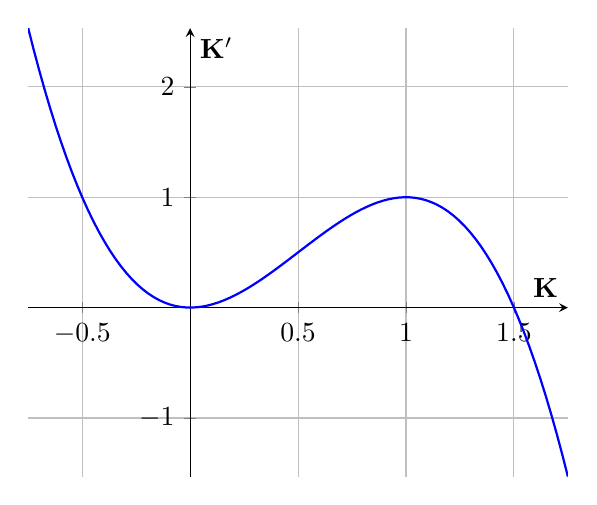
\begin{tikzpicture}
        \begin{axis}[
                axis lines = middle,
                xlabel = {$\vK$},
                ylabel = {$\vK'$},
                domain=-0.75:1.75,
                samples=100,
                grid=both,
            ]
            \addplot[
                color=blue,
                thick
            ]{3*x^2-2*x^3};
        \end{axis}
    \end{tikzpicture}
    \caption{Plot of $\vK' = 3 \vK^2 - 2 \vK^3$ in the case $\vK$ is scalar.}
    \label{fig:plot-g}
\end{figure}

In general, we place no restrictions on the matrix ${\vK \in \mathbb{R}^{m \times m}}$. In particular, it might not be directly diagonalizable. It is well known, however, that for every square matrix $\vK$ there exists an invertible matrix $\vP$ and a Jordan normal form \cite{jordan-form} $\vJ \in \mathbb{C}^{m \times m}$ of ${\vK \in \mathbb{R}^{m \times m}}$ such that ${\vK = \vP \vJ \vP^{-1}}$. From this the dual problem,
\begin{align}
    \vJ = 3 \vJ^2 - 2 \vJ^3,
\end{align}
can be constructed. Let $d_\lambda$ denotes the algebraic multiplicity of eigenvalue $\lambda$ of $\vK$. Then, the block-diagonal structure of $\vJ$ imposes up to four equations per eigenvalue of $\vK$ (see Appendix \ref{app:jordan}):
\begin{align}
    \lambda & = 3\lambda^2 - 2\lambda^3 & \label{eq:cond1}                                   \\
    1       & = 6\lambda - 6\lambda^2   & \text{Only when $d_\lambda\geq2$.}\label{eq:cond2} \\
    0       & = 3 - 6\lambda            & \text{Only when $d_\lambda\geq3$.}\label{eq:cond3} \\
    0       & = 0 - 2                   & \text{Only when $d_\lambda\geq4$.}\label{eq:cond4}
\end{align}

Clearly, this system of equations is inconsistent when ${d_{\lambda} \geq 2}$, hence geometric multiplicity of every eigenvalue must also be exactly 1. Together this implies that $\vJ$ is diagonalizable for any fixed point $\vK$. Furthermore, the solutions which satisfy only Eq. (\ref{eq:cond1}) are:
%
\begin{align}
    \lambda \in \{0, 0.5, 1\}.
\end{align}

Therefore, any fixed point of ${\vK = 3 \vK^2 - 2 \vK^3}$ must have eigenvalues in this set. Consequently, all idempotent matrices are fixed points, but there exists also non-idempotent fixed points.

Although the initial derivation of ${g(\vK) = 3 \vK^2 - 2 \vK^3}$ relies on $\vK$ being near-idempotent to the first order, we consider more generally the behaviour of $g$ around the fixed points when applied repeatedly as a recurrence relation. Let ${h(\lambda) = 3\lambda^2 - 2\lambda^3}$ and observe its derivative ${h'(\lambda) = 6\lambda - 6\lambda^2}$. Then, for each fixed point of $g$ we have
\begin{align}
    h'(0) = 0, \quad h'(0.5) = 1.5, \quad h'(1) = 0.
\end{align}

Since ${|h'(\lambda)| < 1}$ for ${\lambda \in \{0, 1\}}$ these points are attracting whilst ${|h'(\lambda)| > 1}$ for ${\lambda = 0.5}$, thus this point is repelling. In other words, if the idempotent corrector $g$, applied as a recurrence relation on $\vK$, converges at some point $\vK'$, then $\vK'$ will be approximately idempotent unless $\vK$ has an eigenvalue of exactly $0.5$.

Furthermore, Figure \ref{fig:fractal} shows the result of applying the idempotent corrector recursively 10 times for each point on the complex plane. The attracting regions around $0$ and $1$ are large, hence any matrix that is ``reasonably close'' to idempotent will be projected onto a (within machine precision) idempotent matrix.

\begin{figure*}[!htp]
    \centering
    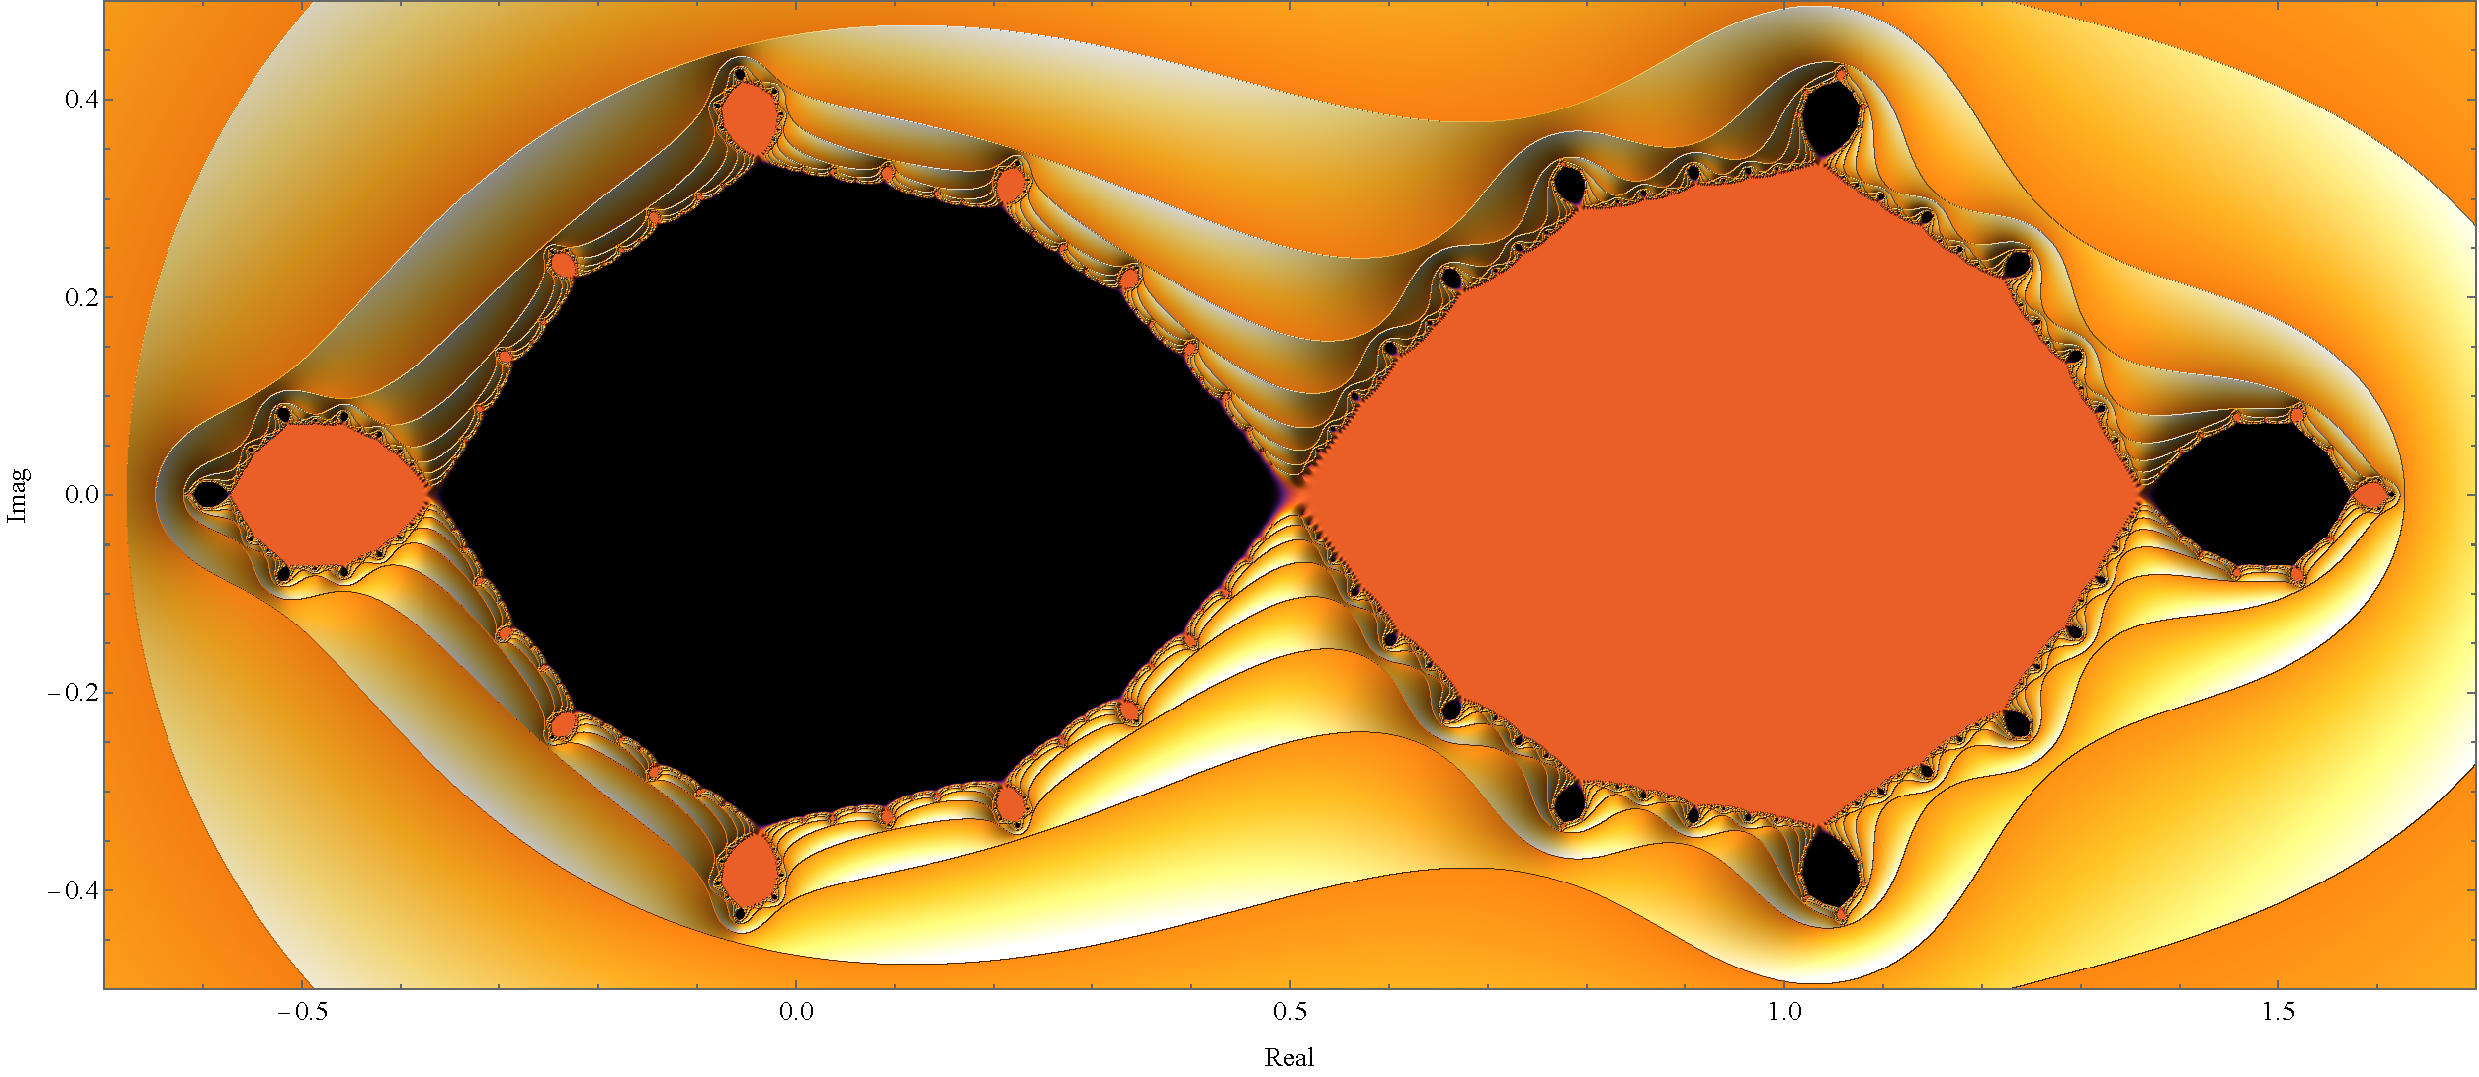
\includegraphics[width=\textwidth]{./resources/fractal.pdf}
    \caption{10-time recursive application of $h(\lambda) = 3\lambda^2 - 2\lambda^3$ for each point on the complex plane. Black areas denote points converging onto $0$, while orange areas denote points converging onto $1$.}
    \label{fig:fractal}
\end{figure*}

Whilst this only technically applies in the linearized setting, we propose to also apply the method in non-linear settings using the following recurrence relation, for $0 \leq \gamma \leq 1$:
%
\begin{align}
    \vK' = \vK + \gamma(g(\vK) - \vK).
\end{align}
%
This has the effect of taking small $\gamma$-sized steps in the direction of $g$ at every time point.

% (1 page)
\subsection{Deriving a Training Scheme}
\label{sec:method-scheme}
Gradient-based optimization techniques use the gradient of an often non-convex loss function as the directional information used to update the hypothesis at each time step. This highlights a core difference between our approach and conventional gradient-based approaches, since the recurrence relation derived above (and shown in Figure \ref{fig:plot-g}) exactly describes the ``direction'' to move in to reduce idempotent error. Our method need only \textit{evaluate} $g$ -- finding its derivative is unimportant.

Consider a neural network ${f_{\vtheta}: \mathbb{R}^m \to \mathbb{R}^m}$ together with its application to input ${\vx \in \mathbb{R}^m}$, denoted ${\vy = f_{\vtheta}(\vx)}$. We might then consider the recurrence relation in Eq. (\ref{eq:g}) in the following form:
%
\begin{align}
    \vy' = 3f_{\vtheta}(\vy) - 2f_{\vtheta}(f_{\vtheta}(\vy))
\end{align}
%
This describes a desired change in the output of the network which we denote ${\Delta f_{\vtheta}(\vx) = \vy' - \vy}$. In other words, ${\Delta f_{\vtheta}(\vx)}$ describes the change in $\vy$ which moves $\vy$ towards an idempotent projection much in the same way that the quantity $\pd{(-\mathcal{L}_{\mathrm{idem}}(\vy))}{\vy}$ describes the direction which reduces the idempotent loss function $\mathcal{L}_{\mathrm{idem}}(\vy)$ in Eq. (\ref{eq:idem-loss}). A central idea presented in this work is therefore the definition
%
\begin{align}
    \pd{(-\mathcal{L}(\vy))}{\vy} \equiv \Delta f_{\vtheta}(\vx)
    \label{eq:substitution}
\end{align}
%
as an alternative quantity to the traditional, analytical solution to $\pd{(-\mathcal{L}(\vy))}{\vy}$. To complete the scheme, we consider how a change in the output $\vy$ can be propagated to a change in the parameters $\vtheta$ of $f_{\vtheta}$. This, however, is a straightforward application of the chain rule as it is calculated conventionally in backpropagation. We use the term ``\textbf{Modified Backpropagation}'' to refer to the canonical backpropagation algorithm with the rule (\ref{eq:substitution}) applied appropriately when computing gradients.

In practice, the definition (\ref{eq:substitution}) can be implemented in common machine learning frameworks, such as Jax\footnote{https://github.com/jax-ml/jax} and PyTorch\footnote{https://pytorch.org} as a user-defined automatic differentiation rule (see Appendix \ref{app:autodiff-rule}).

% (3 pages)
\section{Experimental Results}
\label{sec:experiment}
%\textit{On experimental networks we give line graphs comparing absolute error at varying learning rates. We also give line graphs for LRs over many epochs. Takeaway message is that for deeper/wider networks we outperform ordinary autodiff by a lot.}
% Outline differences in training scheme.
% Error across LR for B3&B4
% Error across Runs for B3&B4
% (PCA analysis graphs)
To evaluate the training scheme suggested in Section \ref{sec:method-scheme} we compare relative performance between the two methods: ``Ordinary Backpropagation'' with the quantity $\pd{(-\mathcal{L}(\vy))}{\vy}$ resolved at runtime by automatic differentiation, and ``Modified Backpropagation'' with the modified backpropagation rule for $\pd{(-\mathcal{L}(\vy))}{\vy}$. To demonstrate the flexibility of the approach, we report results for four diverse MLP-style networks, as described in table \ref{tab:networks}.

The dataset used for training in this section is drawn from a normal distribution with mean $0$ and standard deviation $1$. To prevent concerns about overfitting, the distribution is sampled i.i.d. at each epoch during training. Furthermore, a batch size of $1000$ is used, although comparable results have been found for batch sizes between $32$ and $10\,000$. The optimizer used is SGD.

\begin{table}[htbp]
    \begin{center}
        \begin{tabular}{|c|p{0.18\textwidth}|c|}
            \hline
            \textbf{Identifier} & \textbf{Architecture}                                                                                                    & \textbf{No. Parameters} \\
            \hline
            \hline
            B1                  & Linear(5, 5)                                                                                                             & $30$                    \\
            \hline
            B2                  & Linear(128, 256) \newline Linear(256, 256) \newline Linear(256, 256) \newline Linear(256, 256) \newline Linear(256, 128) & $263\,296$              \\
            \hline
            B3                  & Linear(4096, 1024) \newline Linear(1024, 4096)                                                                           & $8\,393\,728$           \\
            \hline
            B4                  & Linear(784, 1024) \newline Linear(1024, 2048) \newline Linear(2048, 784)                                                 & $4\,509\,456$           \\
            \hline
        \end{tabular}
        \vspace{5pt}
        \caption{Four neural networks for testing. Each ``Linear($n$, $m$)'' block is parameterized by its input dimension $n$ and its output dimension $m$, corresponding to the underlying $\vW \in \mathbb{R}^{m \times n}$ weight matrix. Every block has an associated bias vector and LeakyReLU($0.2$) activation function. B1 represents a trivial network, B2 represents a relatively deep network, B3 represents a relatively wide network, and B4 represents a more realistic network.}
        \label{tab:networks}
    \end{center}
\end{table}

%Runs which result in null matrices are filtered out (so are identities).
%Can we put more results for all networks for tanh and sigmoid in an appendix?

\subsection{Qualitative differences}
\label{sec:experiment-qual}
%\textit{TODO: Include a section on qualitative differences in behaviour of modified and ordinary backpropagation. Does one method travel a different route in the loss landscape? This small section is to be suggestive of distinguishing features of the new method.}
%
In this section we present suggestive evidence that Modified Backpropagation searches the solution space differently from Ordinary Backpropagation.
%
\begin{figure}[h]
    \centering
    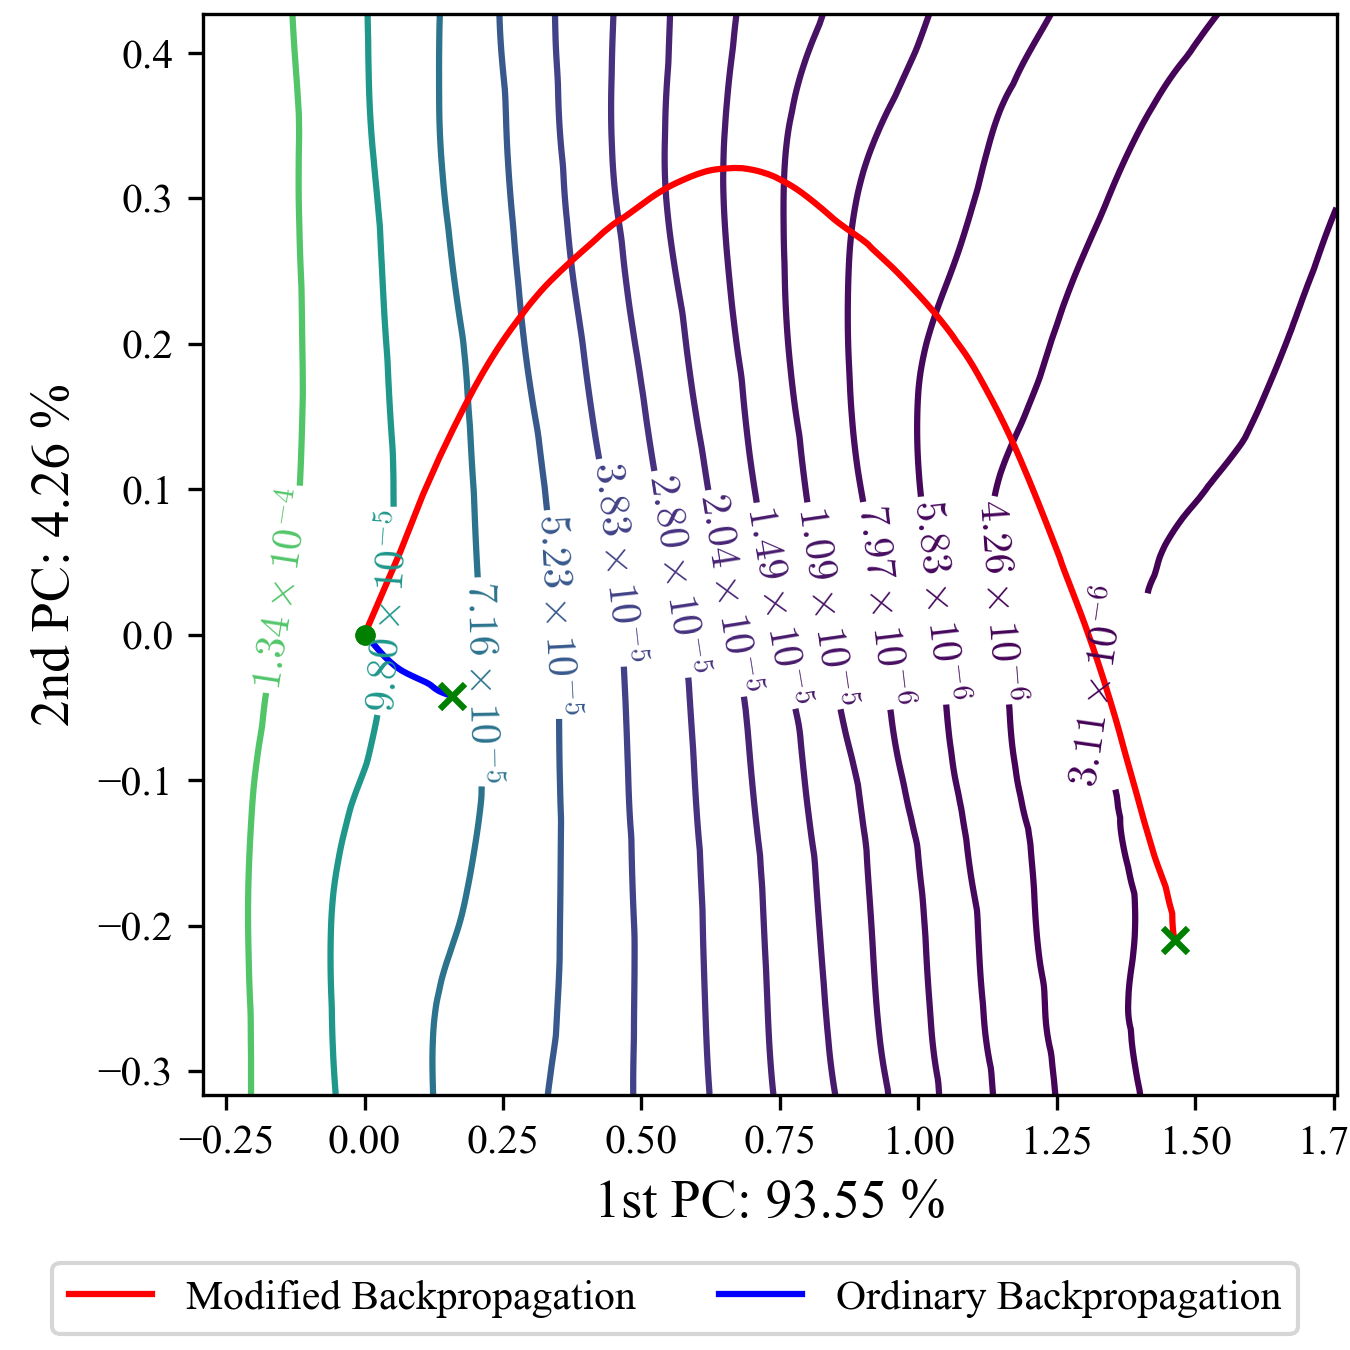
\includegraphics[width=0.9\columnwidth]{./resources/pca_b2.png}
    \caption{Representative projections of the optimizer trajectories over 2500 epochs of either algorithm on the B2 model at optimal learning rates (Figure \ref{fig:avg-abs-err}). Total variance captured is $>97.8\%$ with cosine similarity of PC1 and PC2 less than $1.0\times10^{-6}$. Optimizer trajectory of Modified Backpropagation deviates significantly from Ordinary Backpropagation.}
    \label{fig:pca-b2}
\end{figure}

For purposes of visualization, we employ the methods of \citealt{li-visualizing} to compare the optimizer trajectories of Modified Backpropagation and Ordinary Backpropagation. Concretely, we train a copy of the same network with either algorithm and record model parameters $\vtheta_t^{\mathrm{MB}}$ and $\vtheta_t^{\mathrm{OB}}$ at epoch $t$. A PCA analysis is then performed over the relative change in parameters from $\vtheta_0^{\mathrm{MB}}$ and $\vtheta_0^{\mathrm{OB}}$ (which are identical), from which we select the two most explanatory directions. Lastly, the loss landscape and trajectory paths $\vtheta_t^{\mathrm{MB}}$ and $\vtheta_t^{\mathrm{OB}}$ are projected onto the selected dimensions. An example is shown in Figure \ref{fig:pca-b2} (and Appendix \ref{app:pca}).

Qualitative evaluation show that Modified and Ordinary Backpropagation often differ significantly in projected trajectories across the two most explanatory directions, but this is not always the case (\textit{e.g.}, B4 in Figure \ref{fig:big-pca}). Additionally, optimization trajectories for Modified Backpropagation can be explained by projection onto two direction with more than $90\%$ variance explained, indicating that it exhibits the same behaviour as Ordinary Backpropagation which has previously been suggested to largely operate in low-dimensional subspaces \cite{li-visualizing,song-subspaces}. One should note, however, that the loss surface is here represented under a dramatic dimensionality reduction which makes further conclusions unreliable.

\begin{figure}[h]
    \centering
    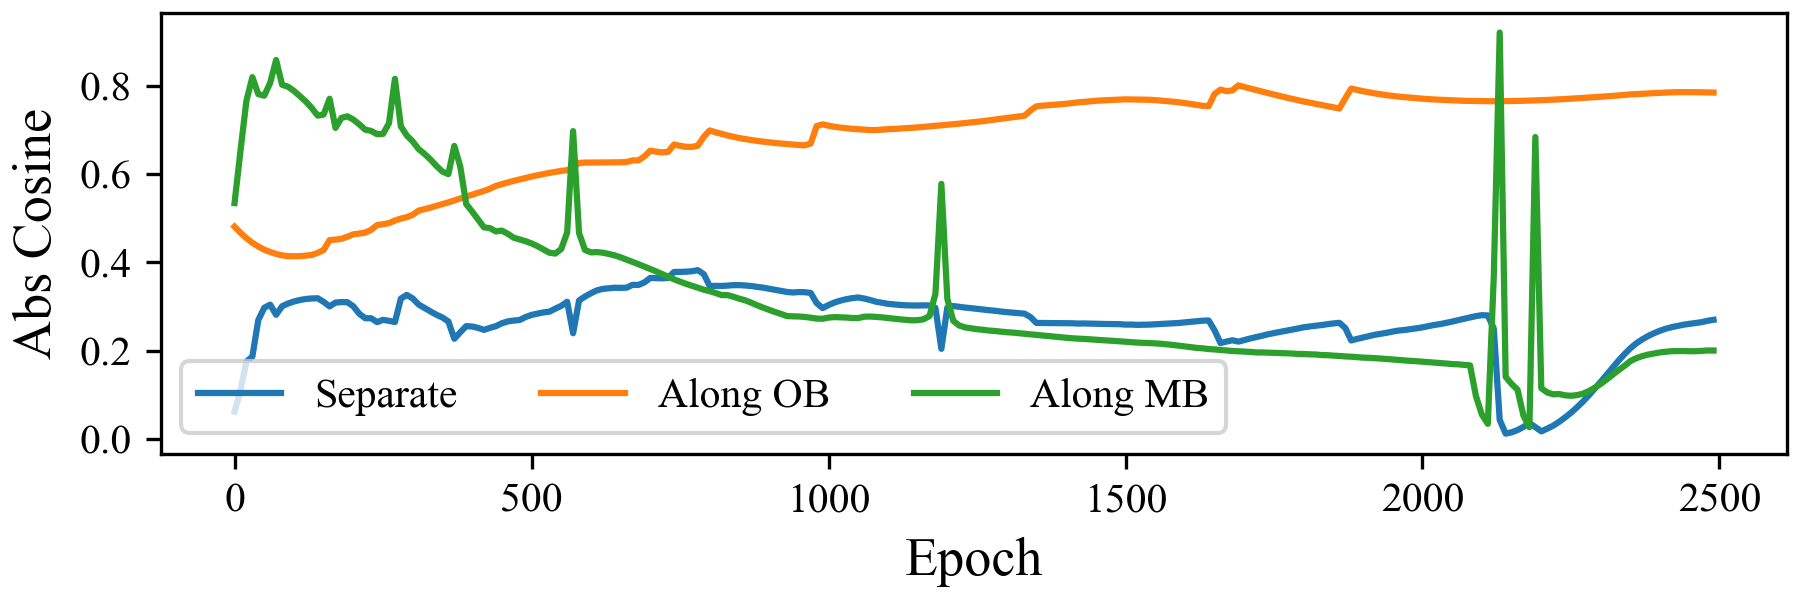
\includegraphics[width=0.95\columnwidth]{./resources/cos.png}
    \caption{Absolute cosine similarity of gradients over time of a representative training run with model B2. ``Along OB'' optimizes the network with Ordinary Backpropagation and compares at each timepoint with suggested gradient from Modified Backpropagation. ``Along MB'' optimizes the network with Modified Backpropagation and compares with suggested gradient from Ordinary Backpropagation. ``Separate'' compares gradients of each optimizer as they independently optimize the network. Gradients suggested by Modified Backpropagation remains significantly different from those suggested by Ordinary Backpropagation.}
    \label{fig:cos-b2}
\end{figure}

\begin{figure}[h]
    \centering
    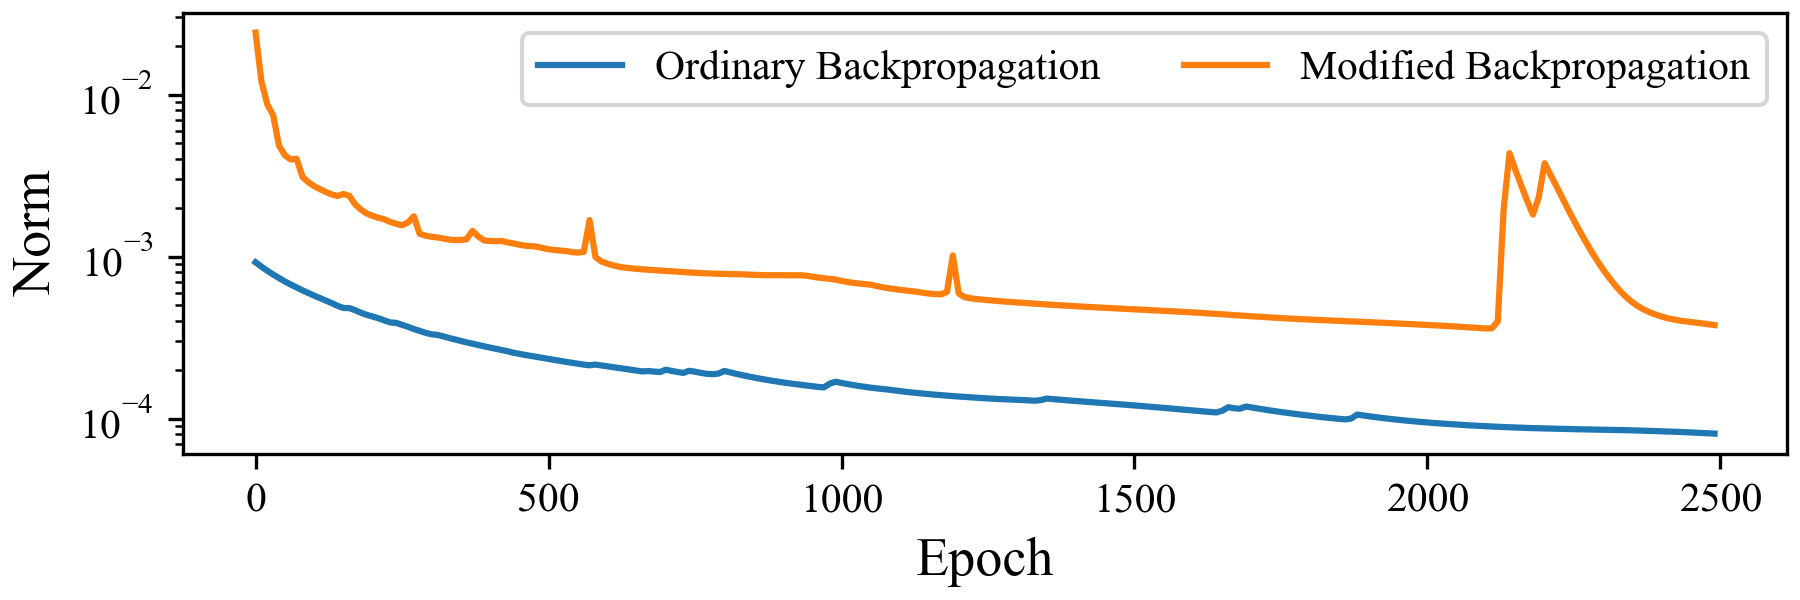
\includegraphics[width=0.95\columnwidth]{./resources/norm.png}
    \caption{Norm of gradients over time of a representative training run with model B2. The network is optimized independently by either algorithm at optimal learning rates (Figure \ref{fig:avg-abs-err}). Modified Backpropagation gives consistently stronger gradient signal than Ordinary Backpropagation.}
    \label{fig:norm-b2}
\end{figure}

We now investigate how the gradients produced by Modified Backpropagation differ from those produced by Ordinary Backpropagation. We give here an analysis over a single training run on network B2, but similar results hold for all networks in table \ref{tab:networks} over repetitions of the experiment. As Figure \ref{fig:cos-b2} shows, gradients suggested by either algorithm remain relatively dissimilar throughout training, which further indicates a difference in the expected optimization trajectory. Furthermore, as evidenced by Figures \ref{fig:pca-b2} and \ref{fig:cos-b2}, Modified Backpropagation travels faster (\textit{i.e.}, gives stronger gradient signal) than Ordinary Backpropagation, even when optimal learning rates are selected for both algorithms.

%\begin{figure*}[htbp]
%    \centering
%    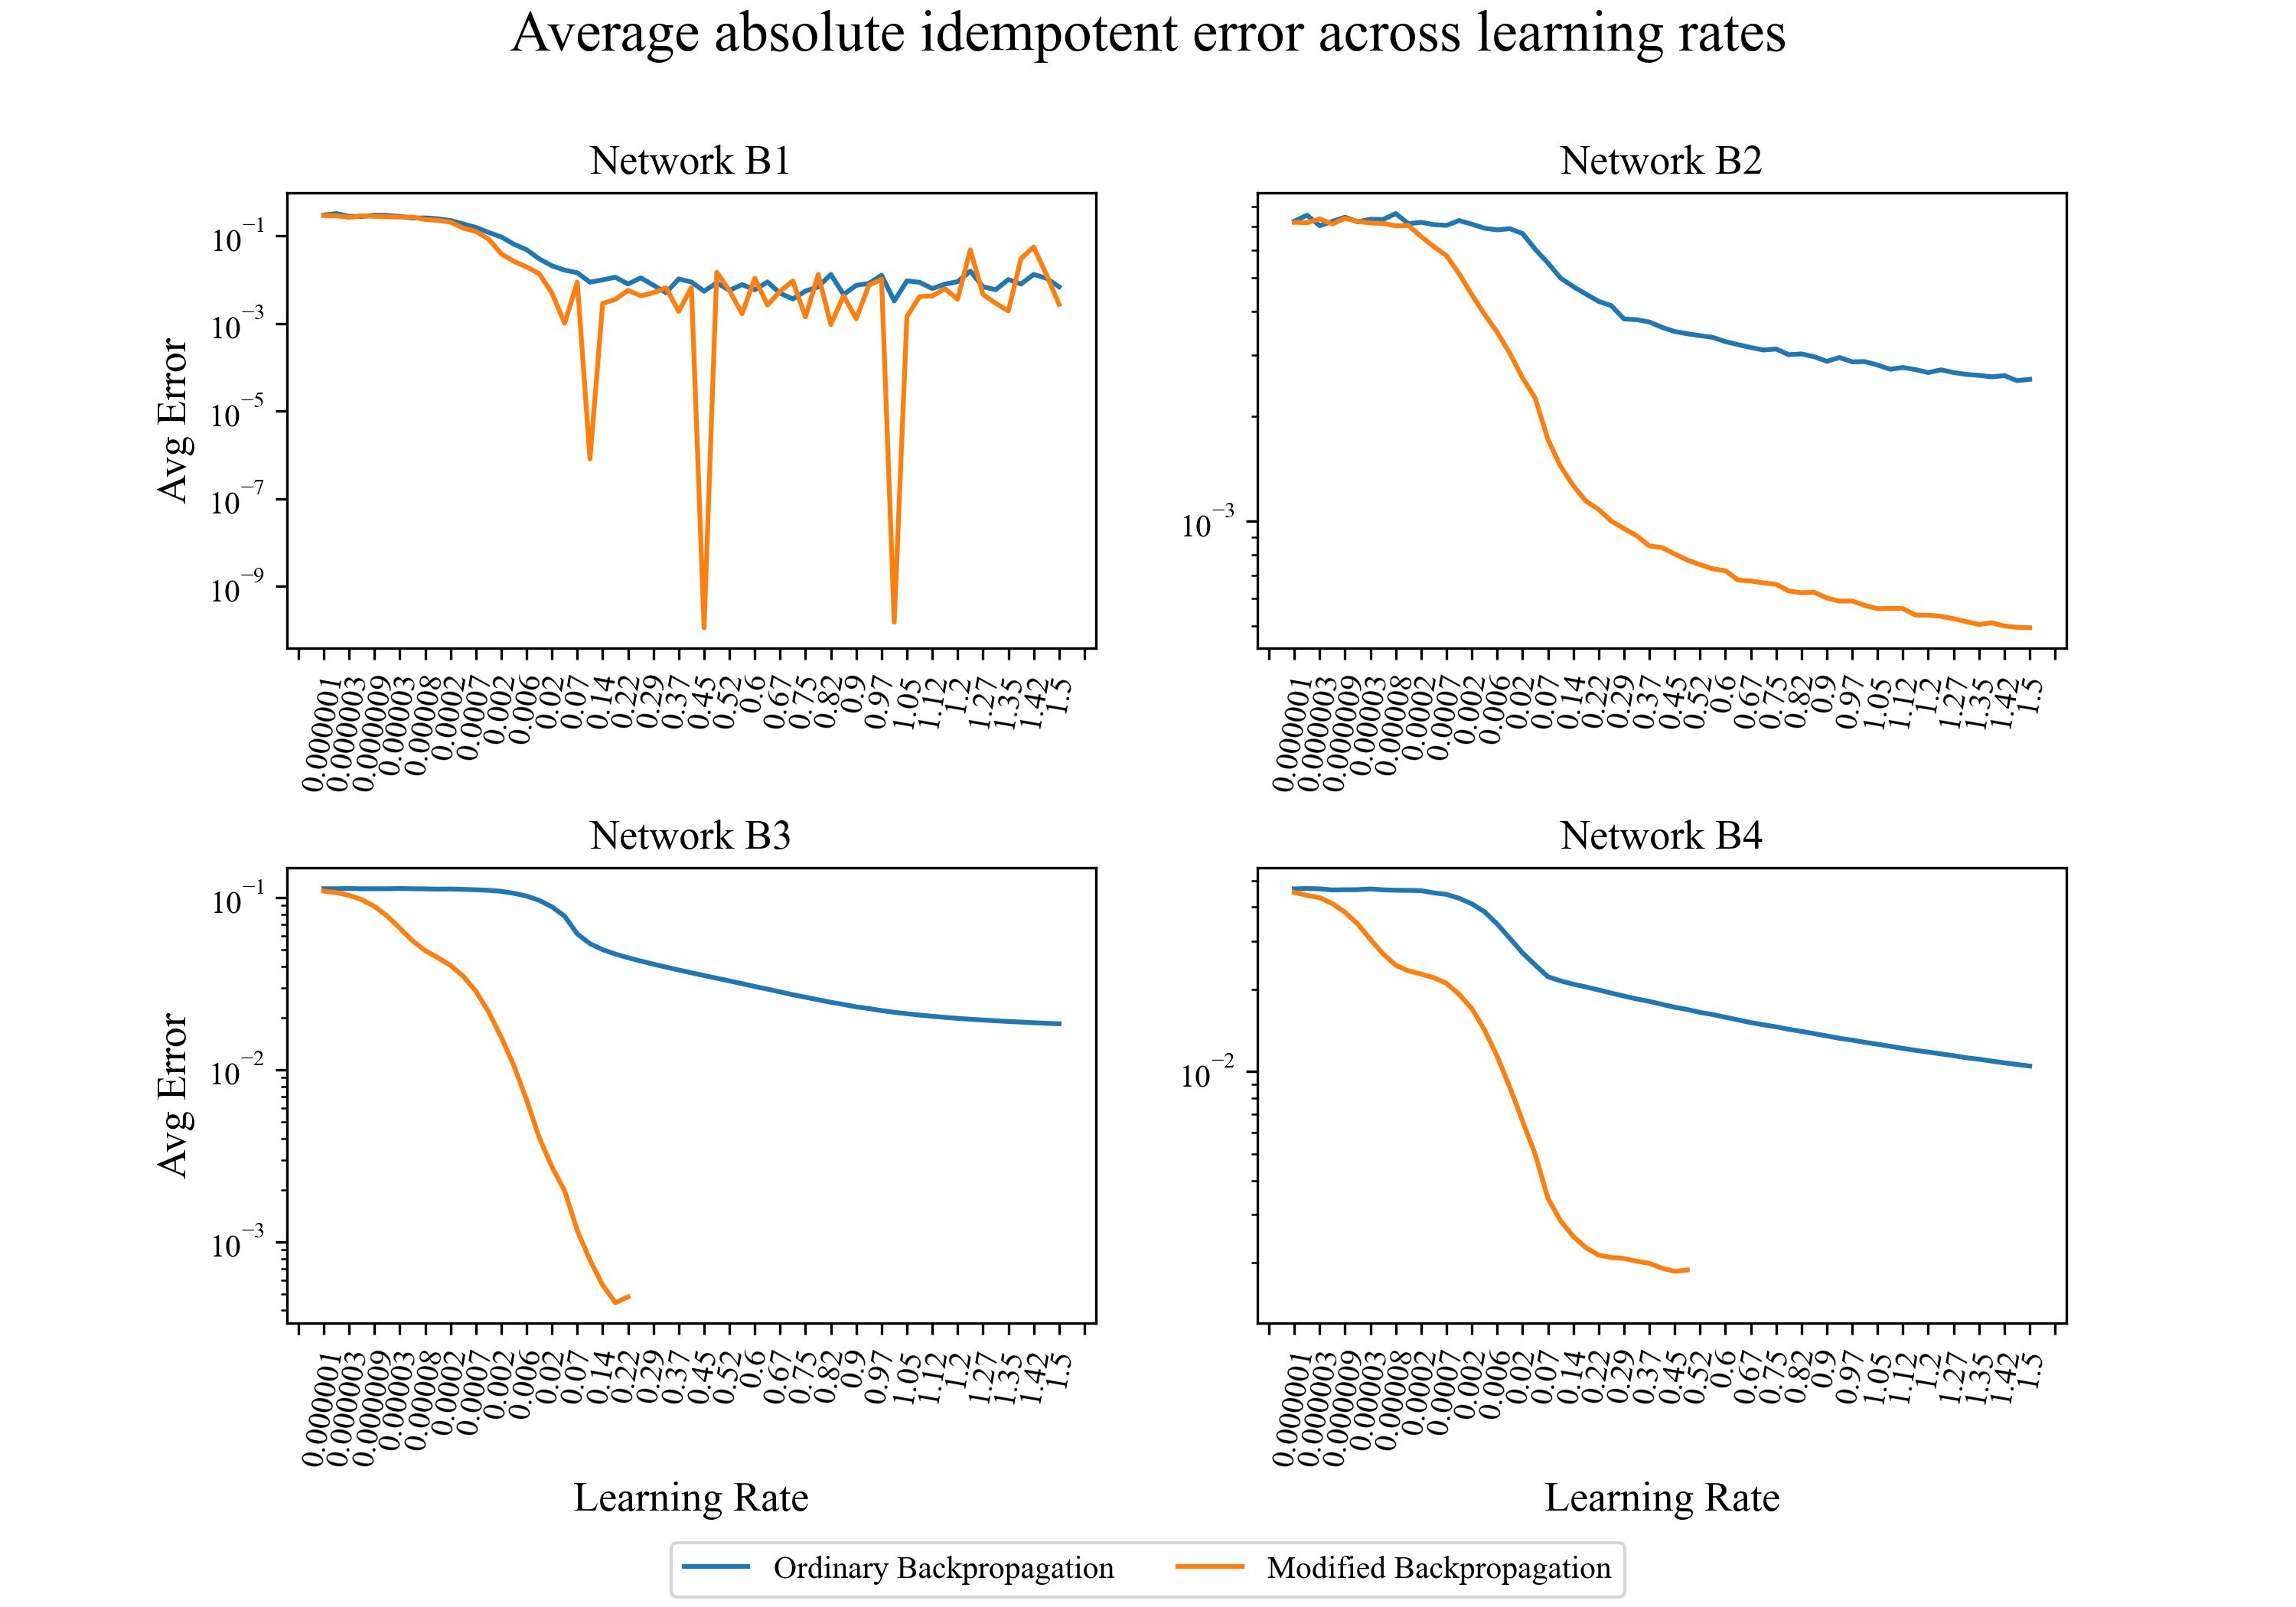
\includegraphics[width=0.5\textwidth]{./resources/abs_err_b1234.png}
%    \caption{Average of 10 runs of each algorithm for a variety of learning rates. Networks are randomly %initialized and trained for $2\,500$ epochs. Runs which did not return a network with lower idempotent %error than the initial value are discarded, and the average is over remaining runs. For networks B3 %and B4, learning rates $>0.22$ and $>0.52$ respectively had no runs with improvement in error. For %Modified Backpropagation on B1, some runs resulted in approximately $\bm{0}$ which, due to %floating-point imprecision, results in the error spikes.}
%    \label{fig:avg-abs-err}
%\end{figure*}
%%
%\begin{figure*}[htbp]
%    \centering
%    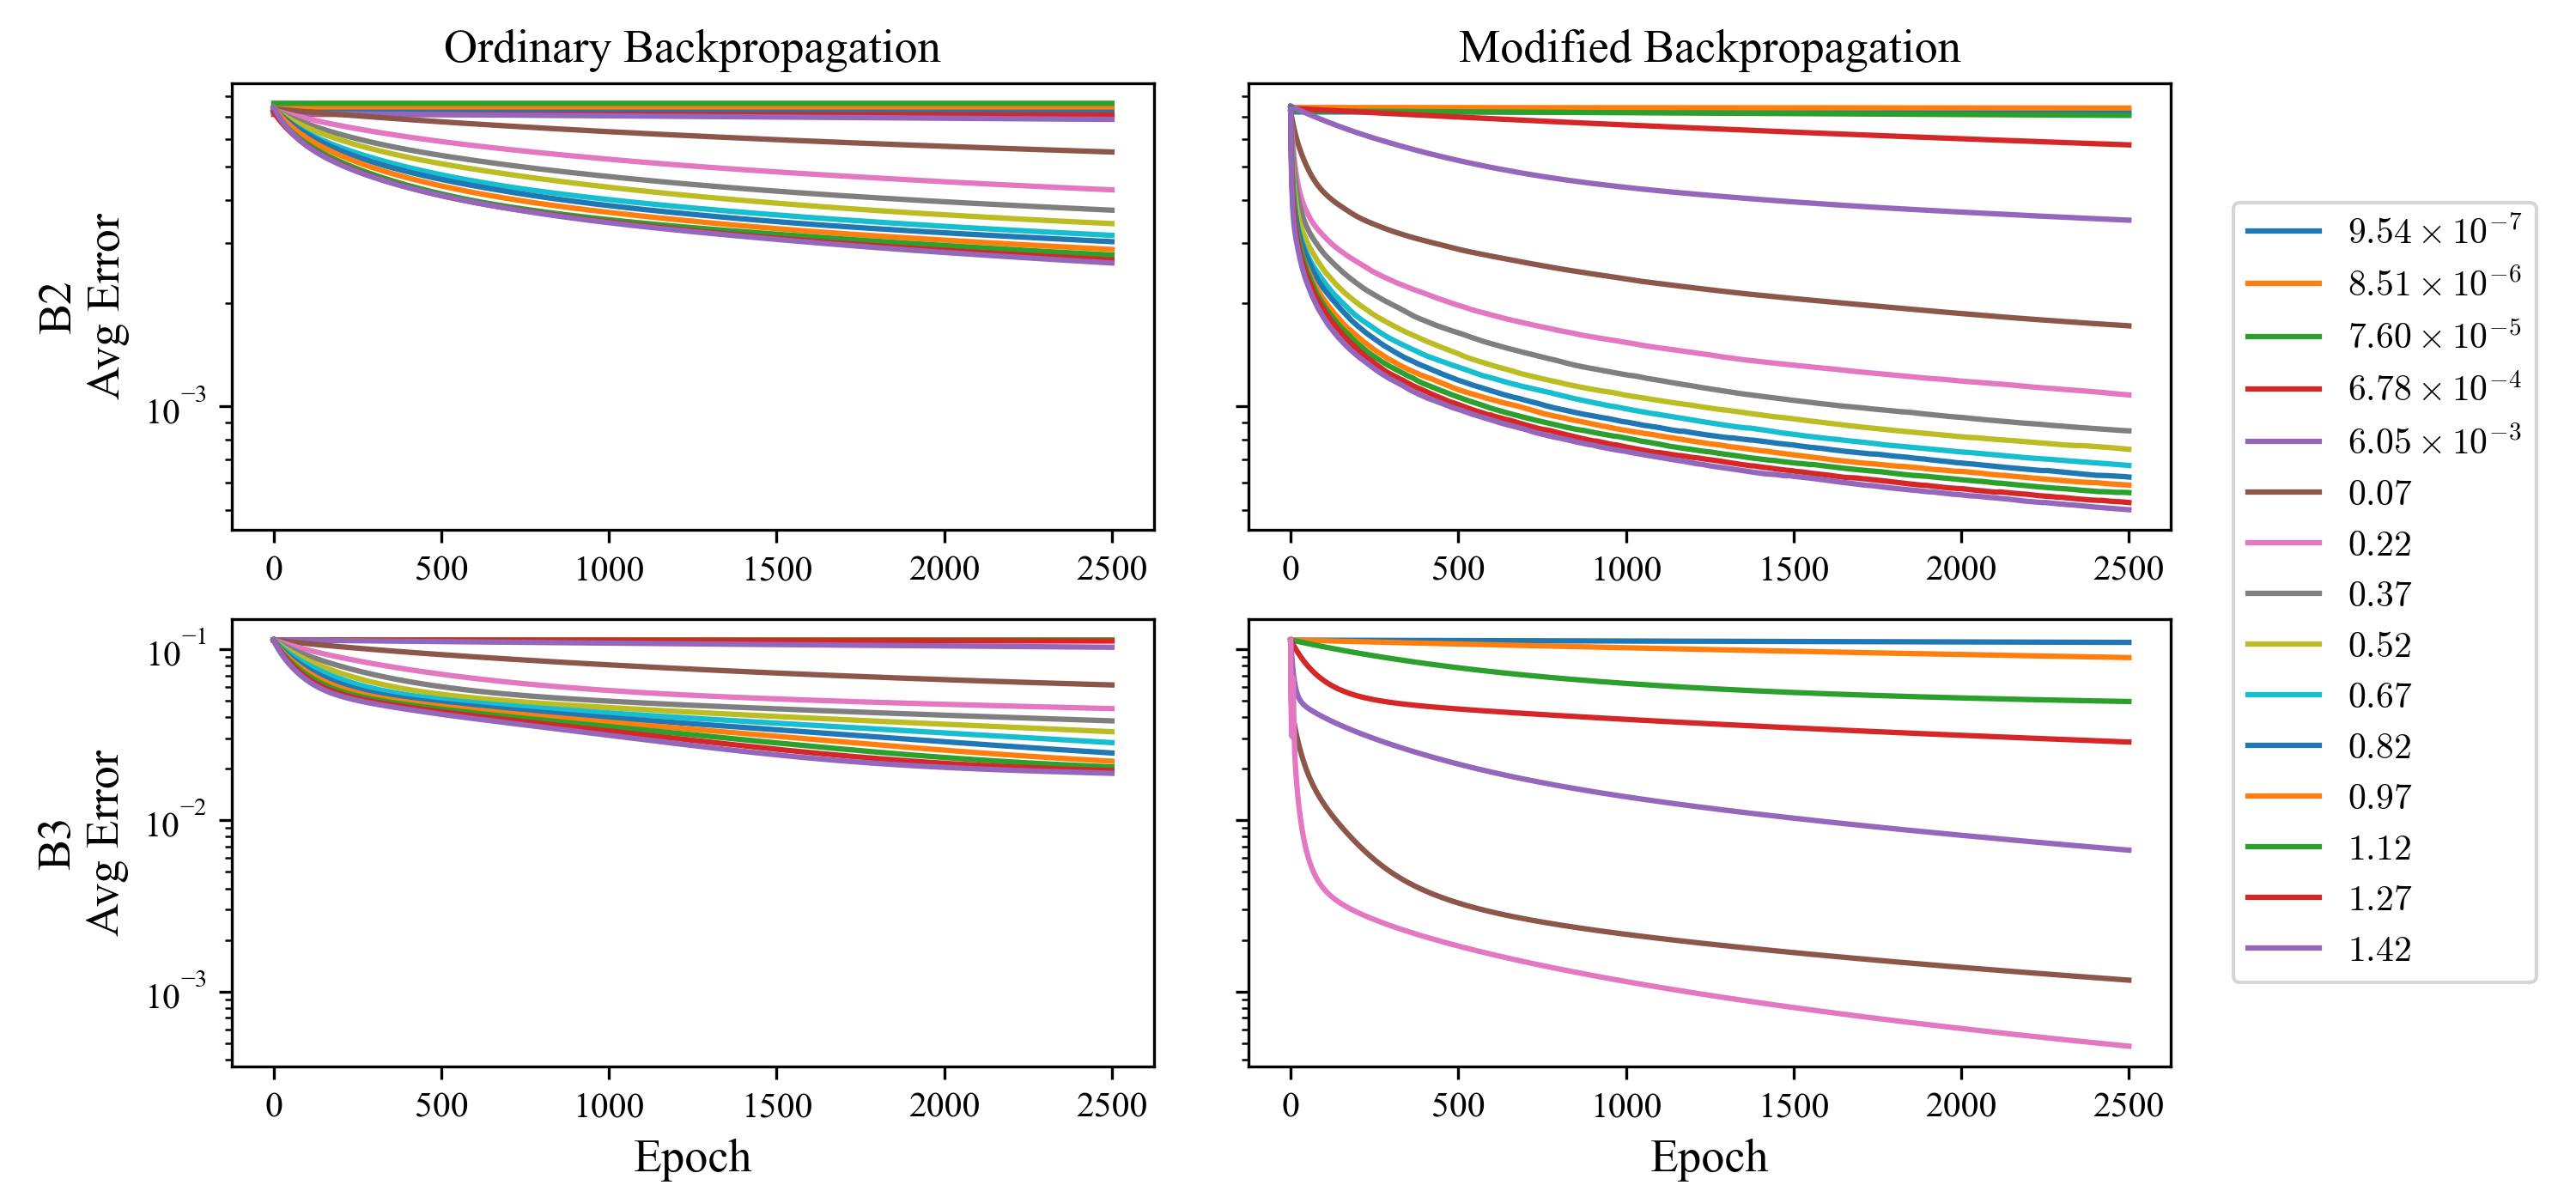
\includegraphics[width=0.5\textwidth]{./resources/runs_err_b23.png}
%    \caption{On networks B2 and B3, the average idempotent error across 10 runs for each learning rate is %reported for each algorithm. Each column of graphs represents one algorithm. Modified Backpropagation %achieves lower idempotent error at lower learning rates than Ordinary Backpropagation. The biggest %relative improvement between algorithms occurs in the first $\sim500$ epochs.}
%    \label{fig:avg-epoch-err}
%\end{figure*}

%\begin{figure*}[!t]
%    \centering
%    \subfigure[Average of 10 runs of each algorithm for a variety of learning rates. Networks are randomly %initialized and trained for $2\,500$ epochs. Runs which did not return a network with lower idempotent %error than the initial value are discarded, and the average is over remaining runs. For networks B3 %and B4, learning rates $>0.22$ and $>0.52$ respectively had no runs with improvement in error. For %Modified Backpropagation on B1, some runs resulted in approximately $\bm{0}$ which, due to %floating-point imprecision, results in the error spikes.]{
%        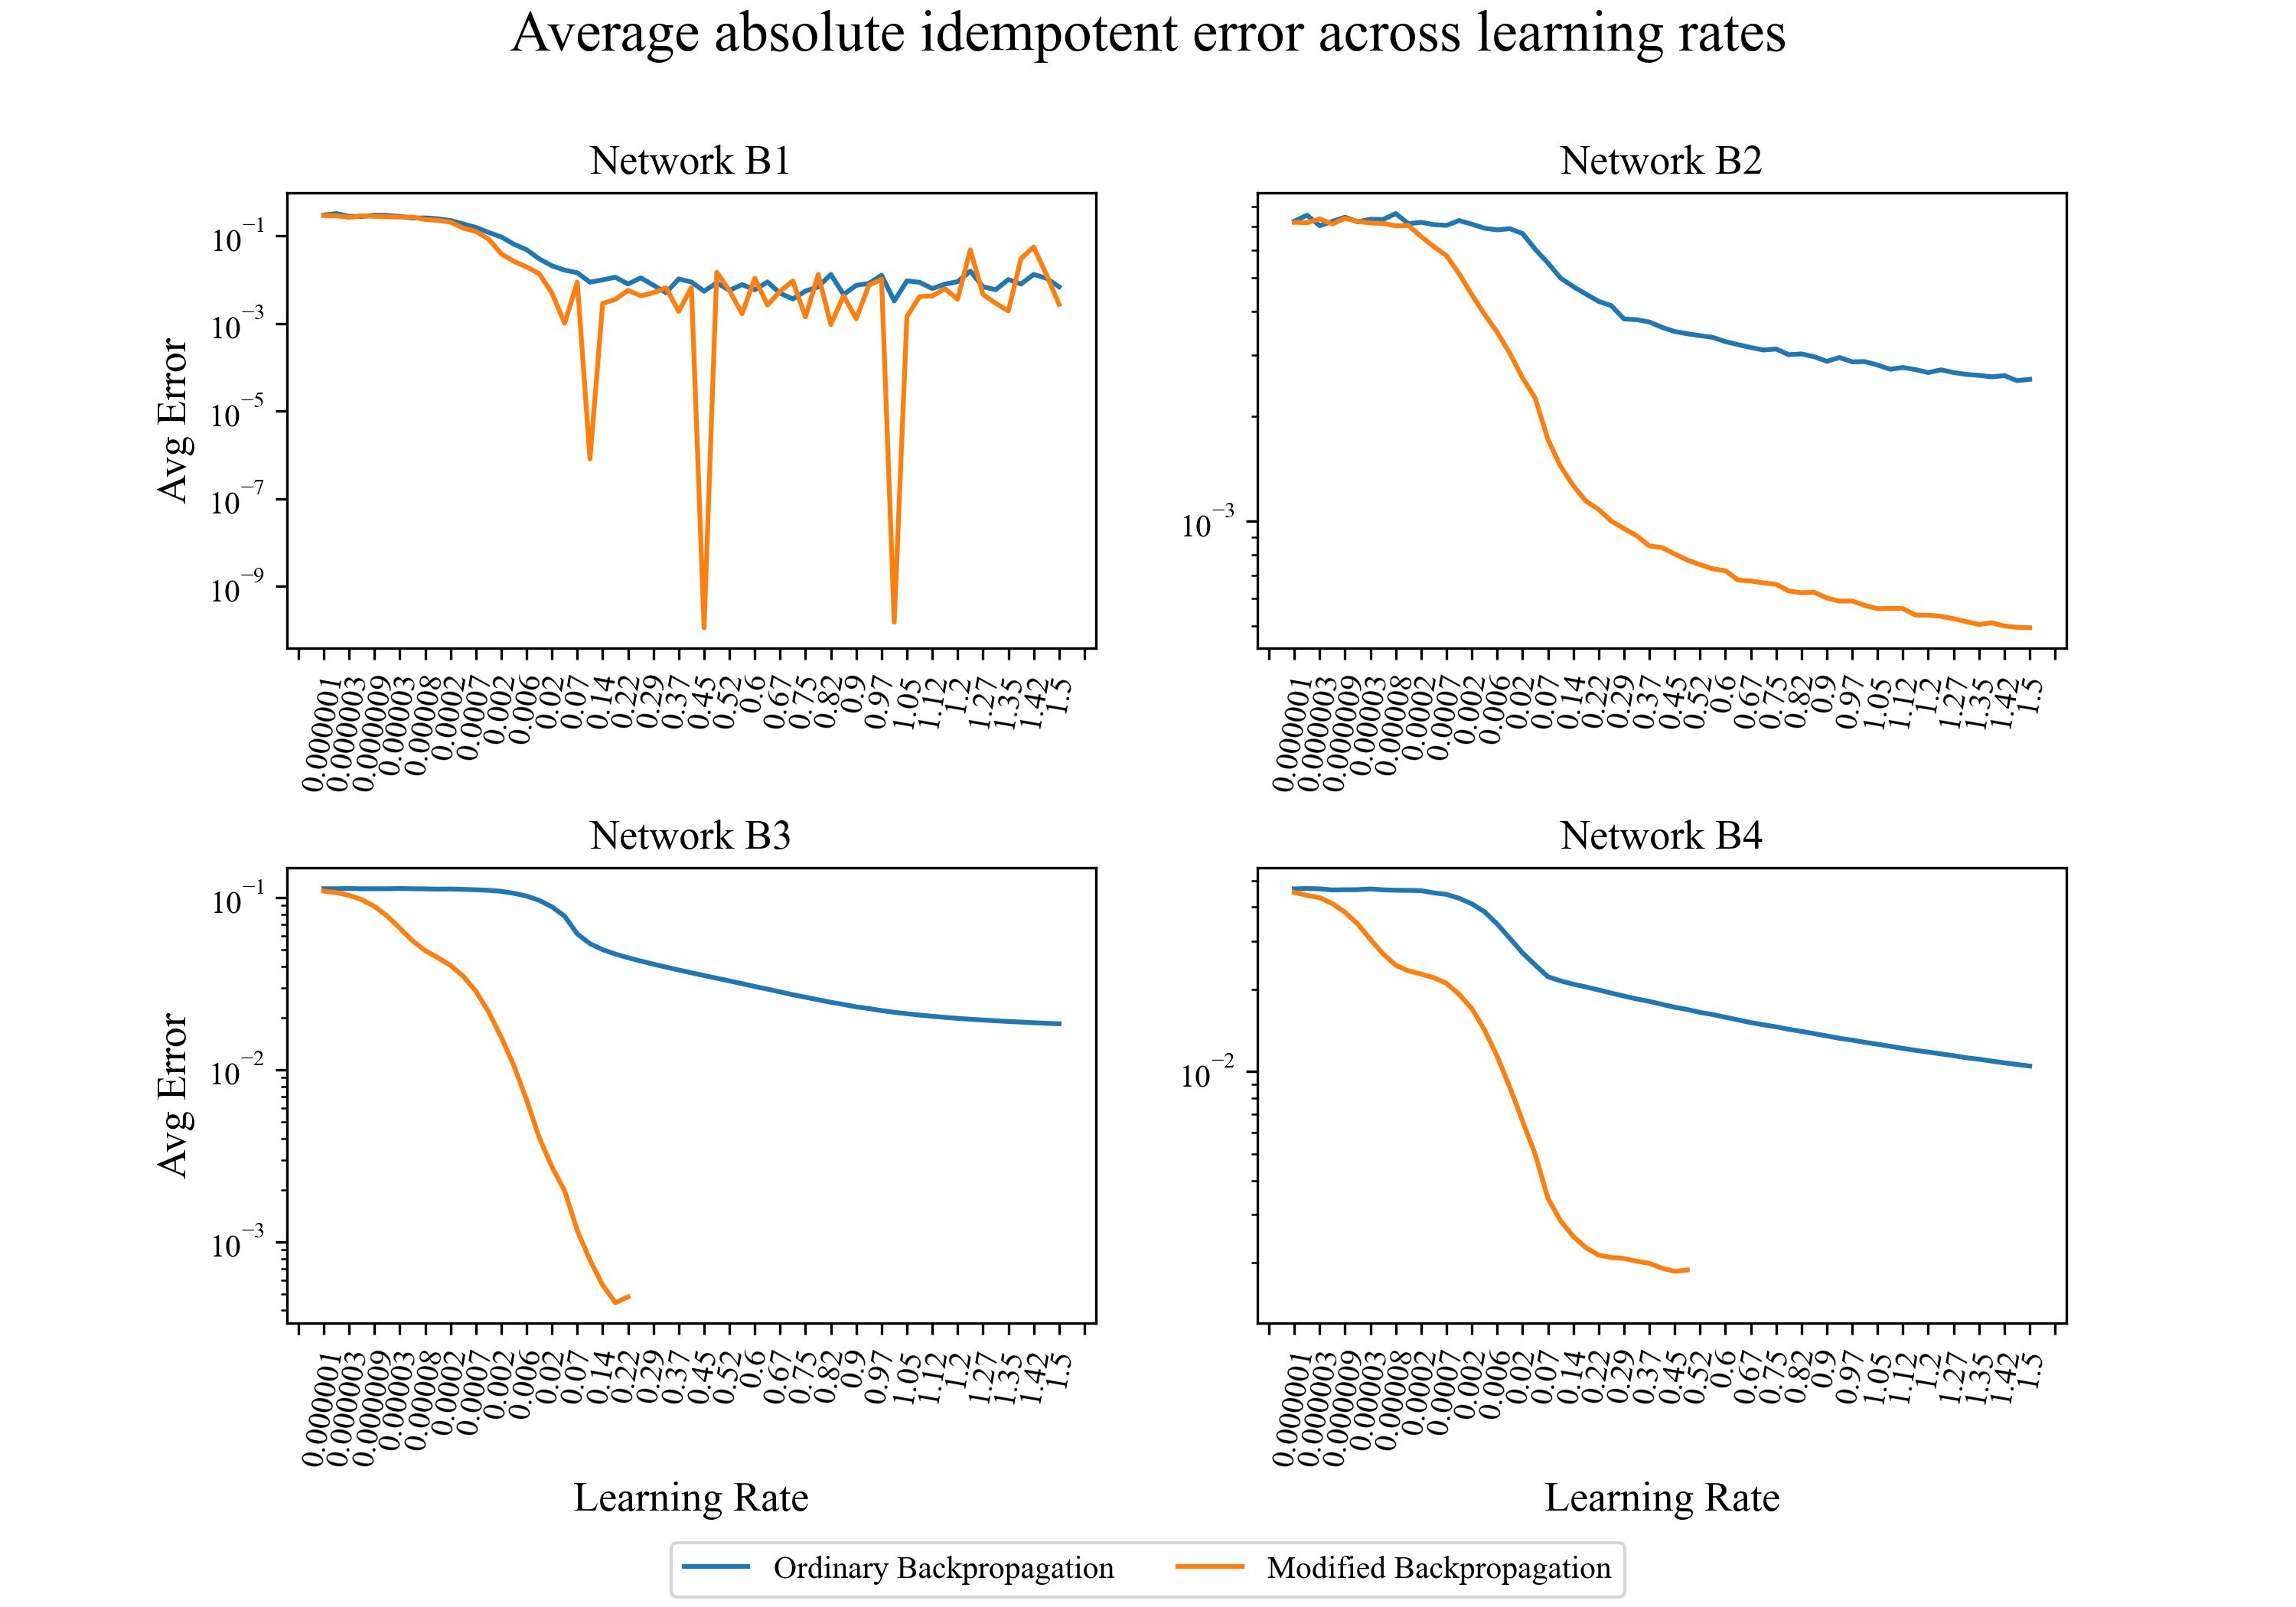
\includegraphics[width=0.9\linewidth]{./resources/abs_err_b1234.png}
%        \label{fig:avg-abs-err}
%    }
%    \subfigure[On networks B2 and B3, the average idempotent error across 10 runs for each learning rate %is reported for each algorithm. Each column of graphs represents one algorithm. Modified %Backpropagation achieves lower idempotent error at lower learning rates than Ordinary Backpropagation. %The biggest relative improvement between algorithms occurs in the first $\sim500$ epochs.]{
%        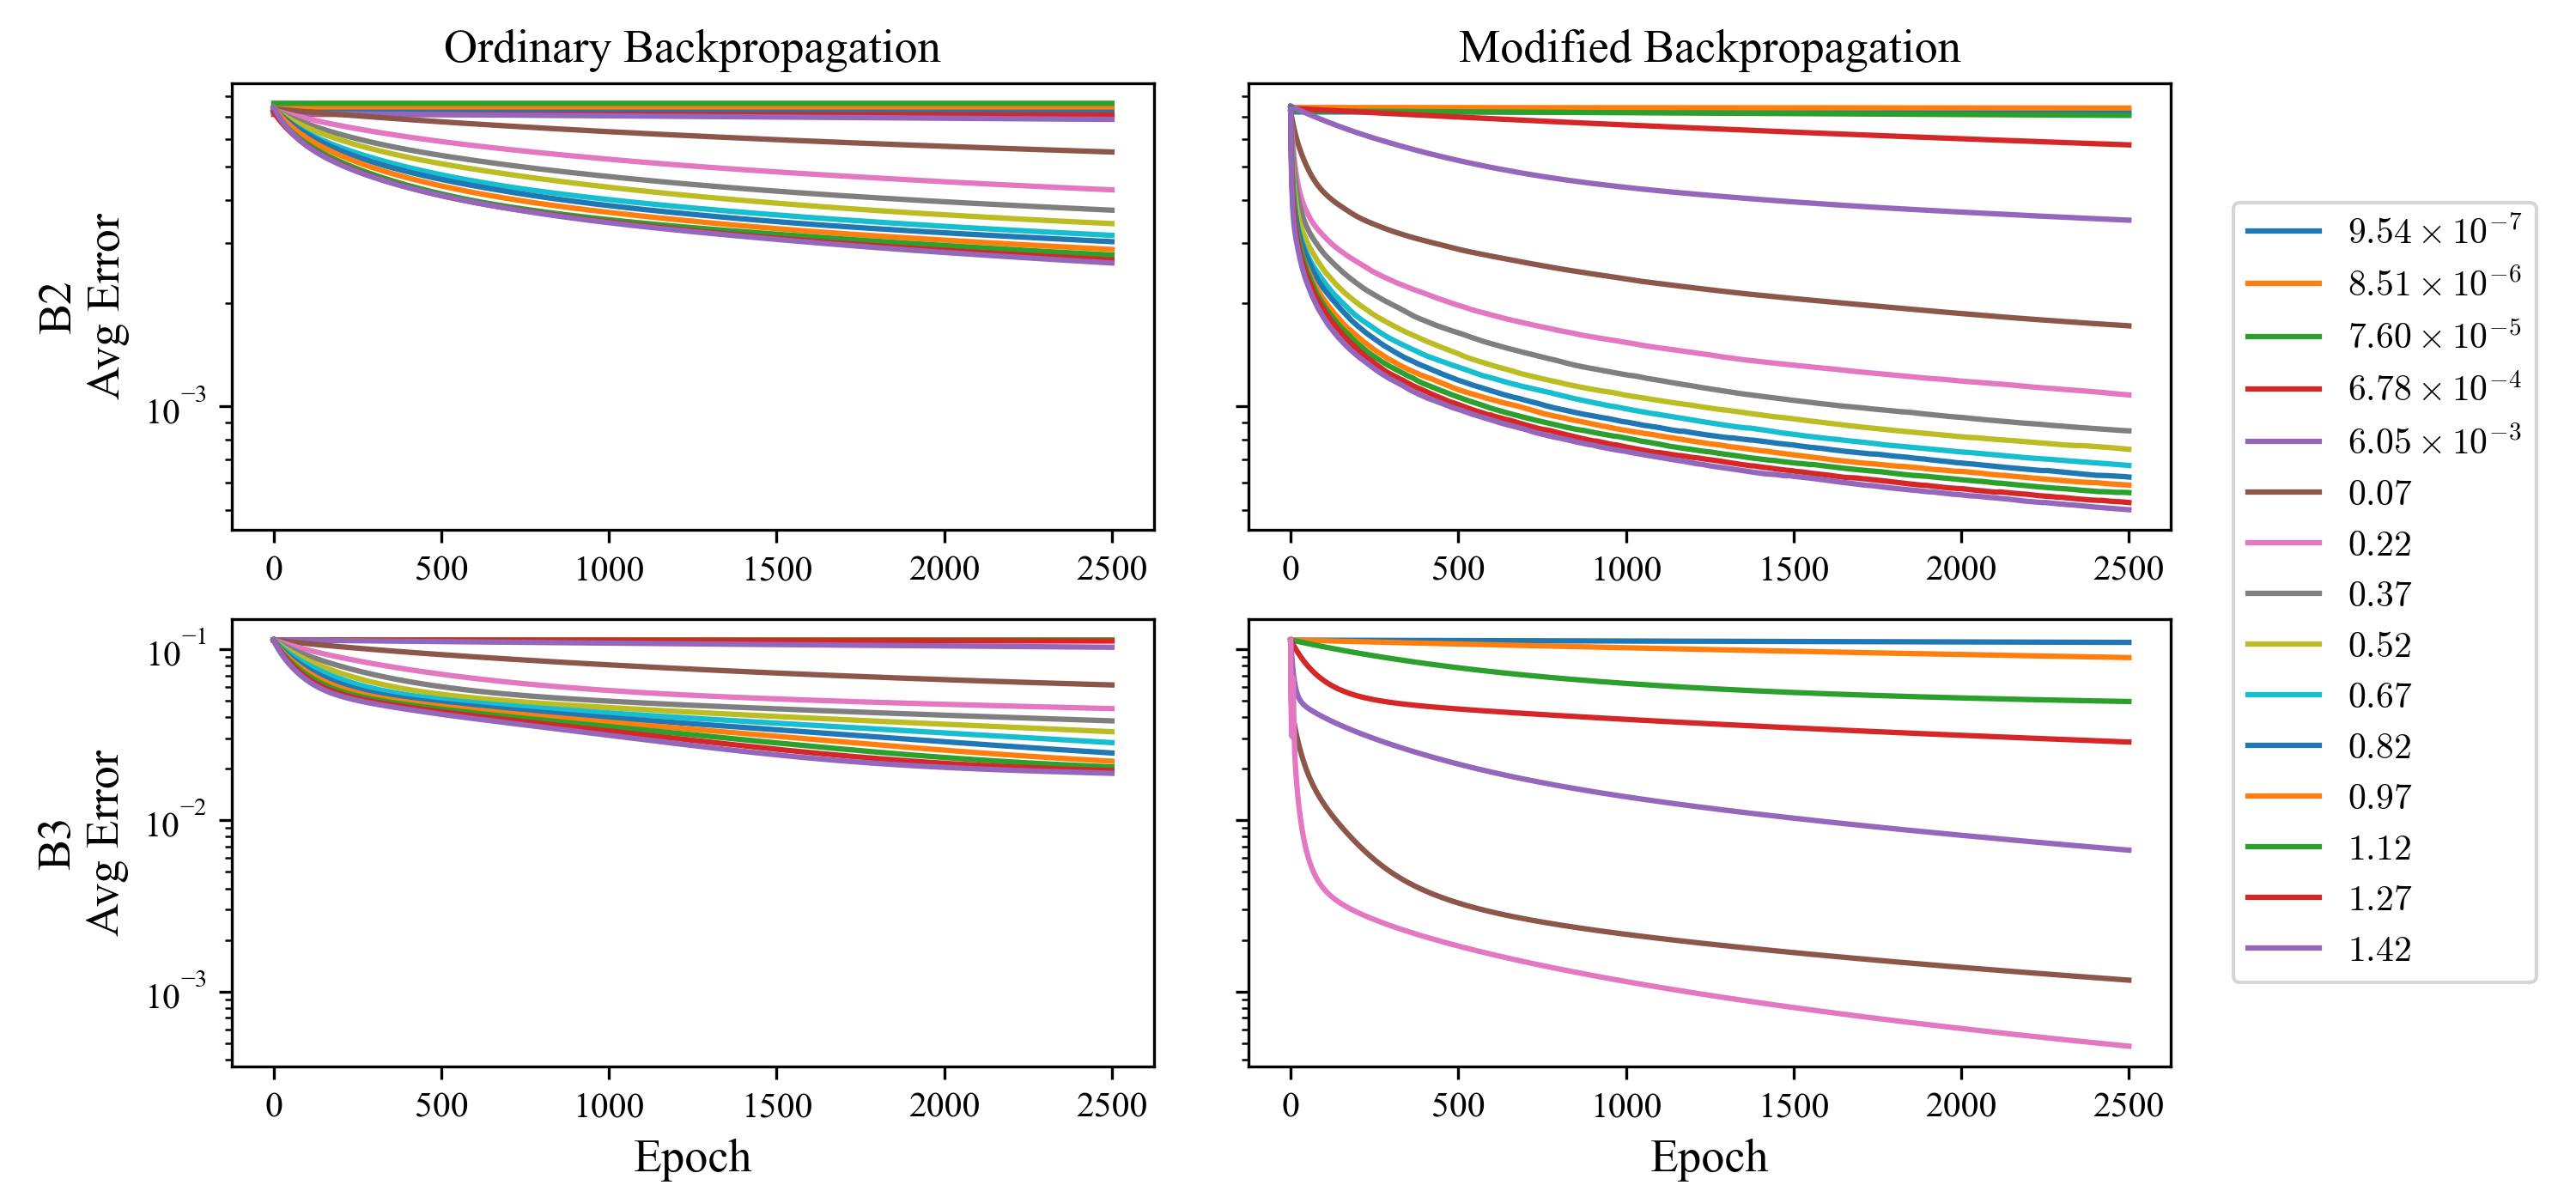
\includegraphics[width=0.8\linewidth]{./resources/runs_err_b23.png}
%        \label{fig:avg-epoch-err}
%    }
%\end{figure*}

\begin{figure*}[!t]
    \centering
    \captionbox{Average of 10 runs of each algorithm for a variety of learning rates. Networks are randomly initialized and trained for $2\,500$ epochs. Runs which did not return a network with lower idempotent error than the initial value are discarded, and the average is over remaining runs. For networks B3 and B4, learning rates $>0.22$ and $>0.52$ respectively had no runs with improvement in error. For Modified Backpropagation on B1, some runs resulted in approximately $\bm{0}$ which, due to floating-point imprecision, results in the error spikes.\label{fig:avg-abs-err}}{
        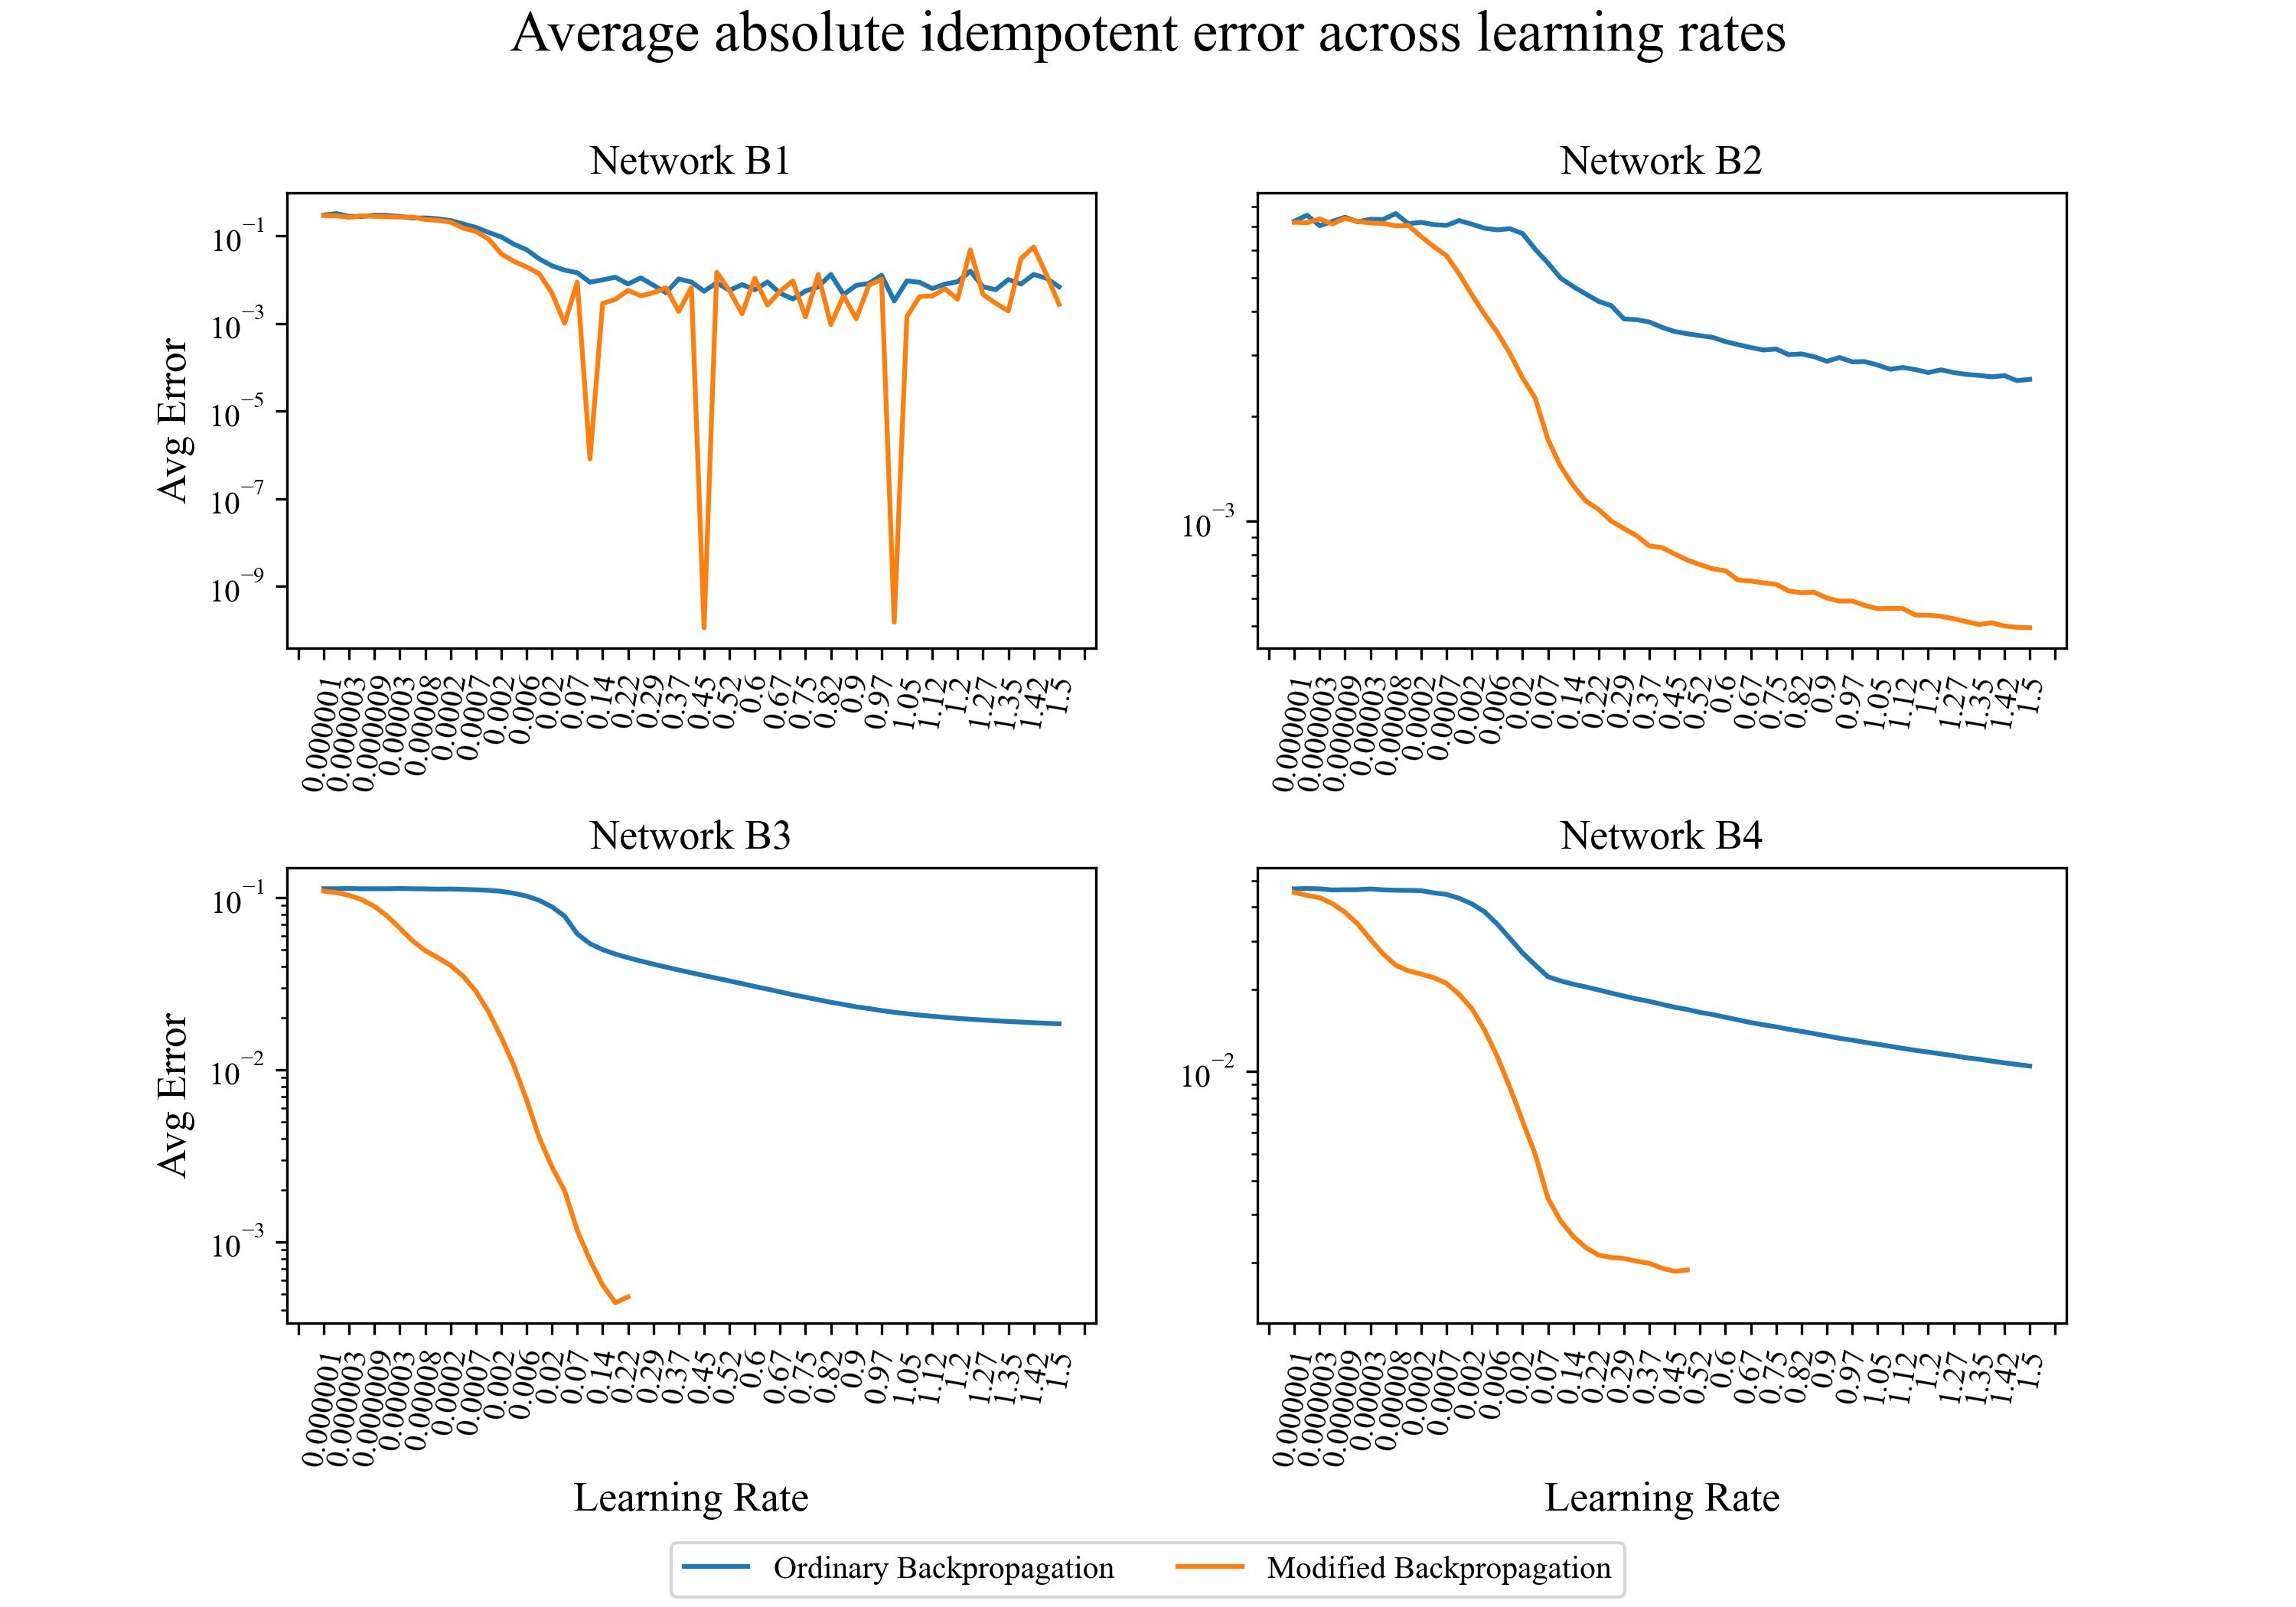
\includegraphics[width=0.9\linewidth]{./resources/abs_err_b1234.png}

    }
    \captionbox{On networks B2 and B3, the average idempotent error across 10 runs for each learning rate is reported for each algorithm. Each column of graphs represents one algorithm. Modified Backpropagation achieves lower idempotent error at lower learning rates than Ordinary Backpropagation. The biggest relative improvement between algorithms occurs in the first $\sim500$ epochs.\label{fig:avg-epoch-err}}{
        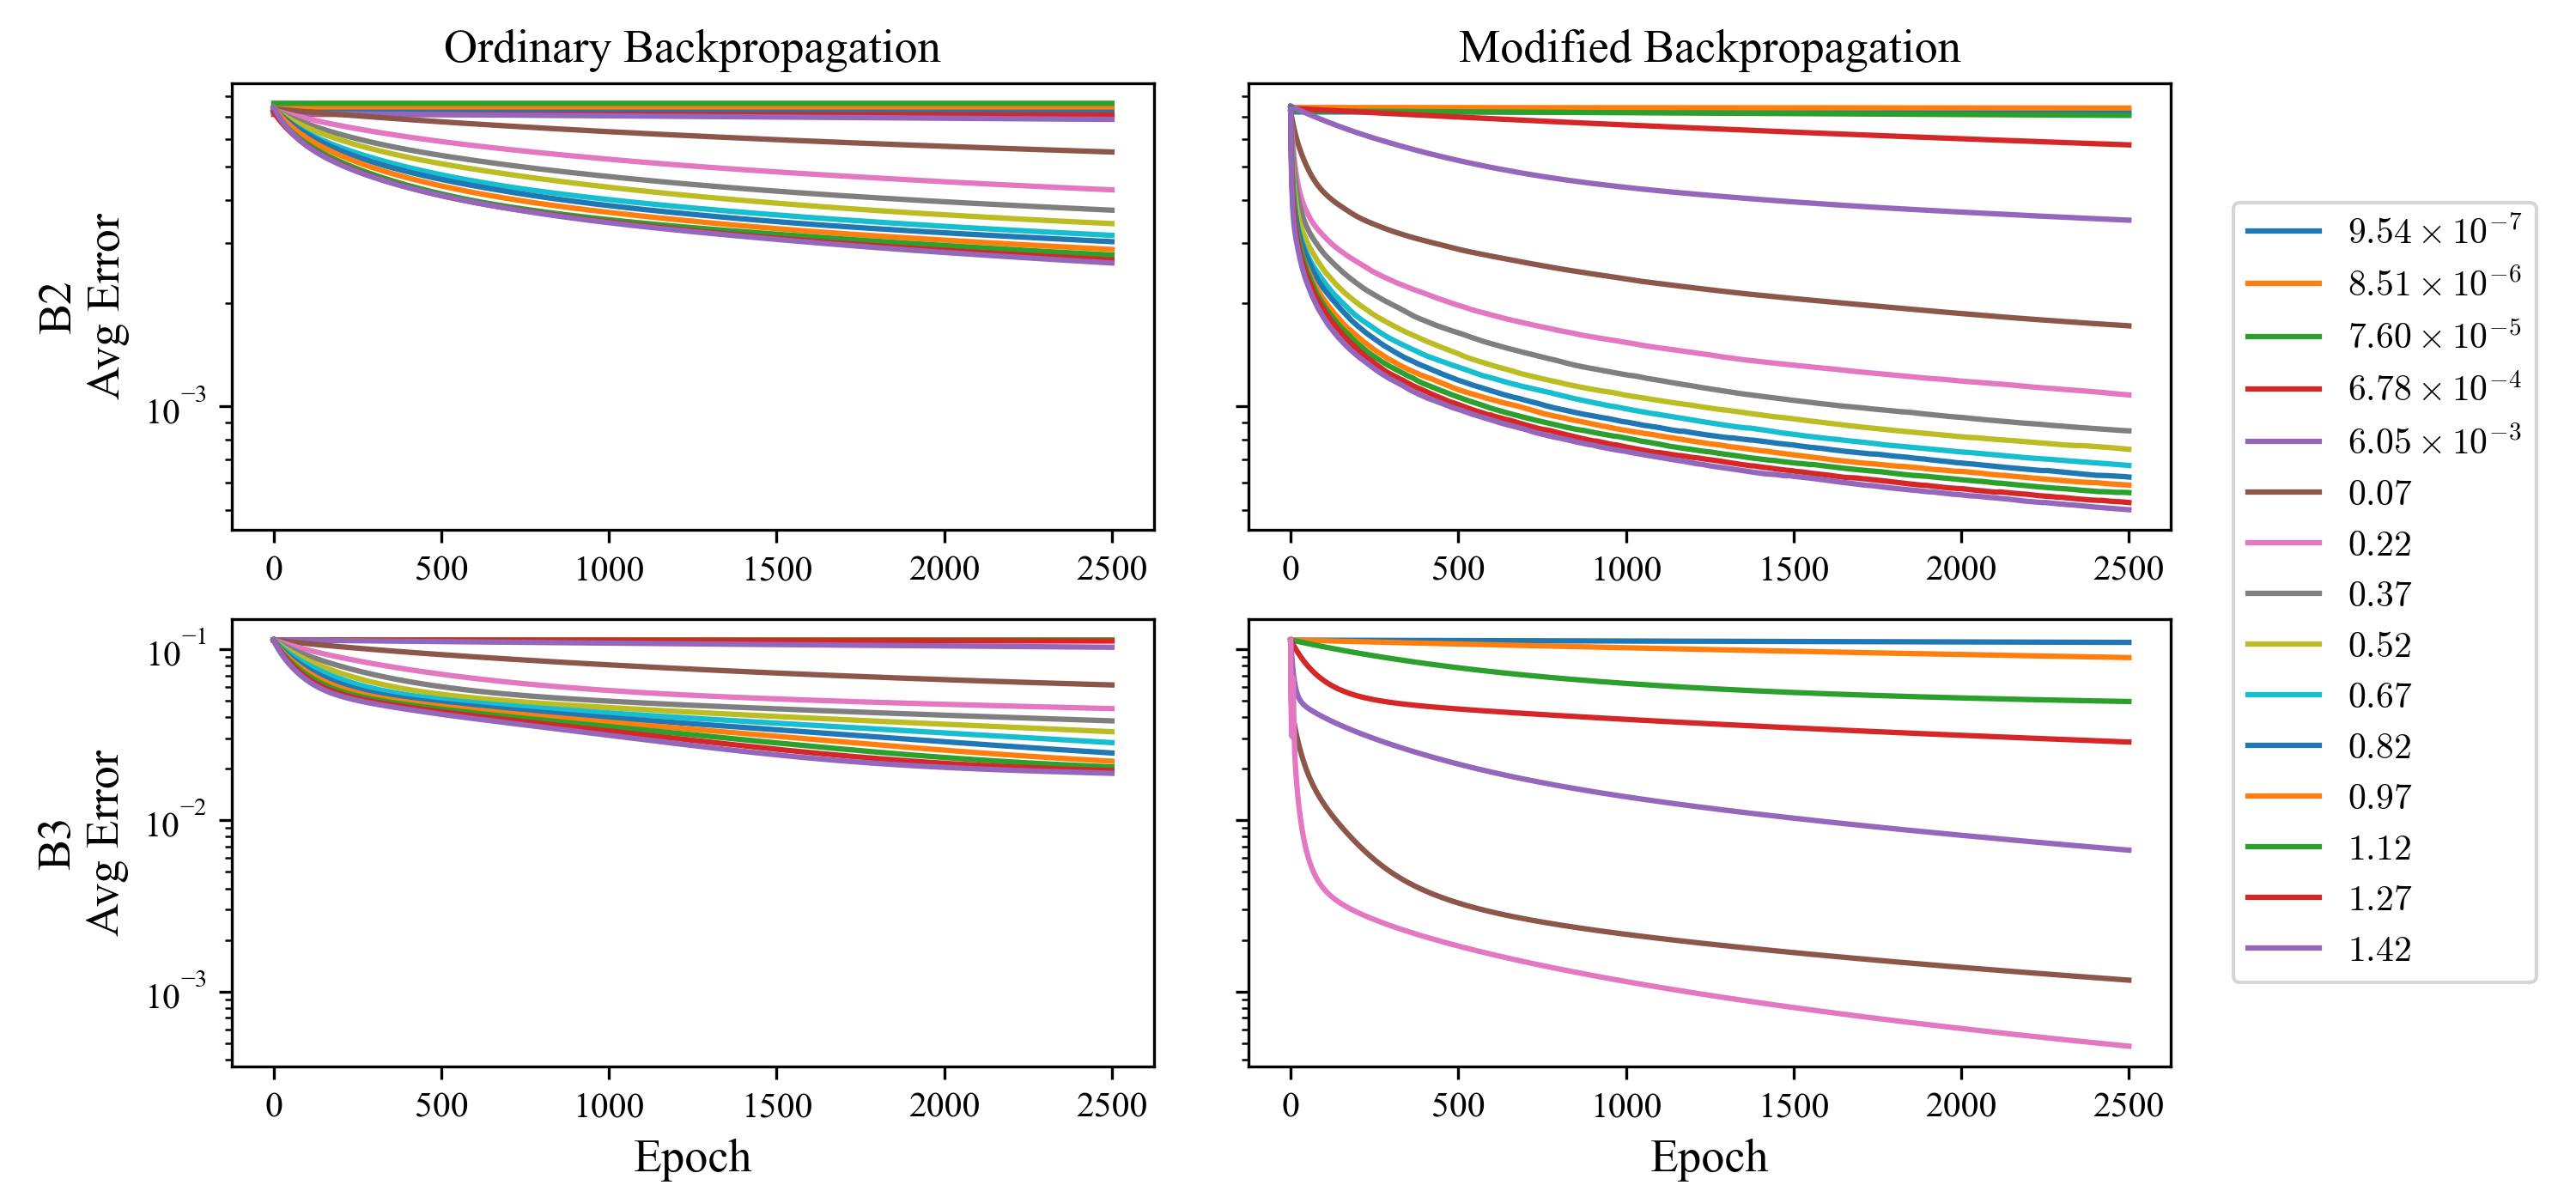
\includegraphics[width=0.8\linewidth]{./resources/runs_err_b23.png}

    }
\end{figure*}

\subsection{Quantitative differences}
\label{sec:experiment-quant}
We now give an evaluation of the relative efficacy of Modified Backpropagation to Ordinary Backpropagation. As shown in Figure \ref{fig:avg-abs-err}, for networks B2-B4 Modified Backpropagation achieves significantly lower absolute idempotent error on average at lower learning rate. For network B3 the difference is more than one order of magnitude. As the tested networks represent varying architectures with a commonly used activation function, these results suggest that Modified Backpropagation fares well in a variety of training configurations.

Although the dataset used here is i.i.d. samples drawn from a Gaussian ${\mathcal{N}(0, 1)}$, we observe similar results when data comes from other distributions, such as the uniform distribution ${\mathcal{U}(-k, k)}$ for ${k \in \mathbb{N}}$. Following \citealt{shocher-ign}, we also observe similar results when applying a Fast Fourier Transform to MNIST data, finding the mean and variance of each frequency, and then apply an inverse FFT to get noise with similar frequency-statistics as the underlying dataset.

Whilst the above results are promising, a natural concern is the quality of solutions produced. In particular, if a significant fraction of networks trained using Modified Backpropagation have weights close to the null matrix $\bm{0}$ or the identity matrix $\vI$ then the algorithm might not be practically useful. We refer the reader to Appendix \ref{app:test-networks-data} which shows that the norm of trained weight matrices in general is comparable to those found by Ordinary Backpropagation.

\begin{figure*}[!b]
    \centering
    \captionbox{Uncurated generations of the U-net style DCGAN model trained on MNIST with Modified Backpropagation for optimizing idempotent and tightness losses. In the top row are samples drawn from a random distribution with mean $0$ and variance $1$, whist the second and third rows represent first and second application of the network to these samples, respectively.\label{fig:gen-mnist}}{
        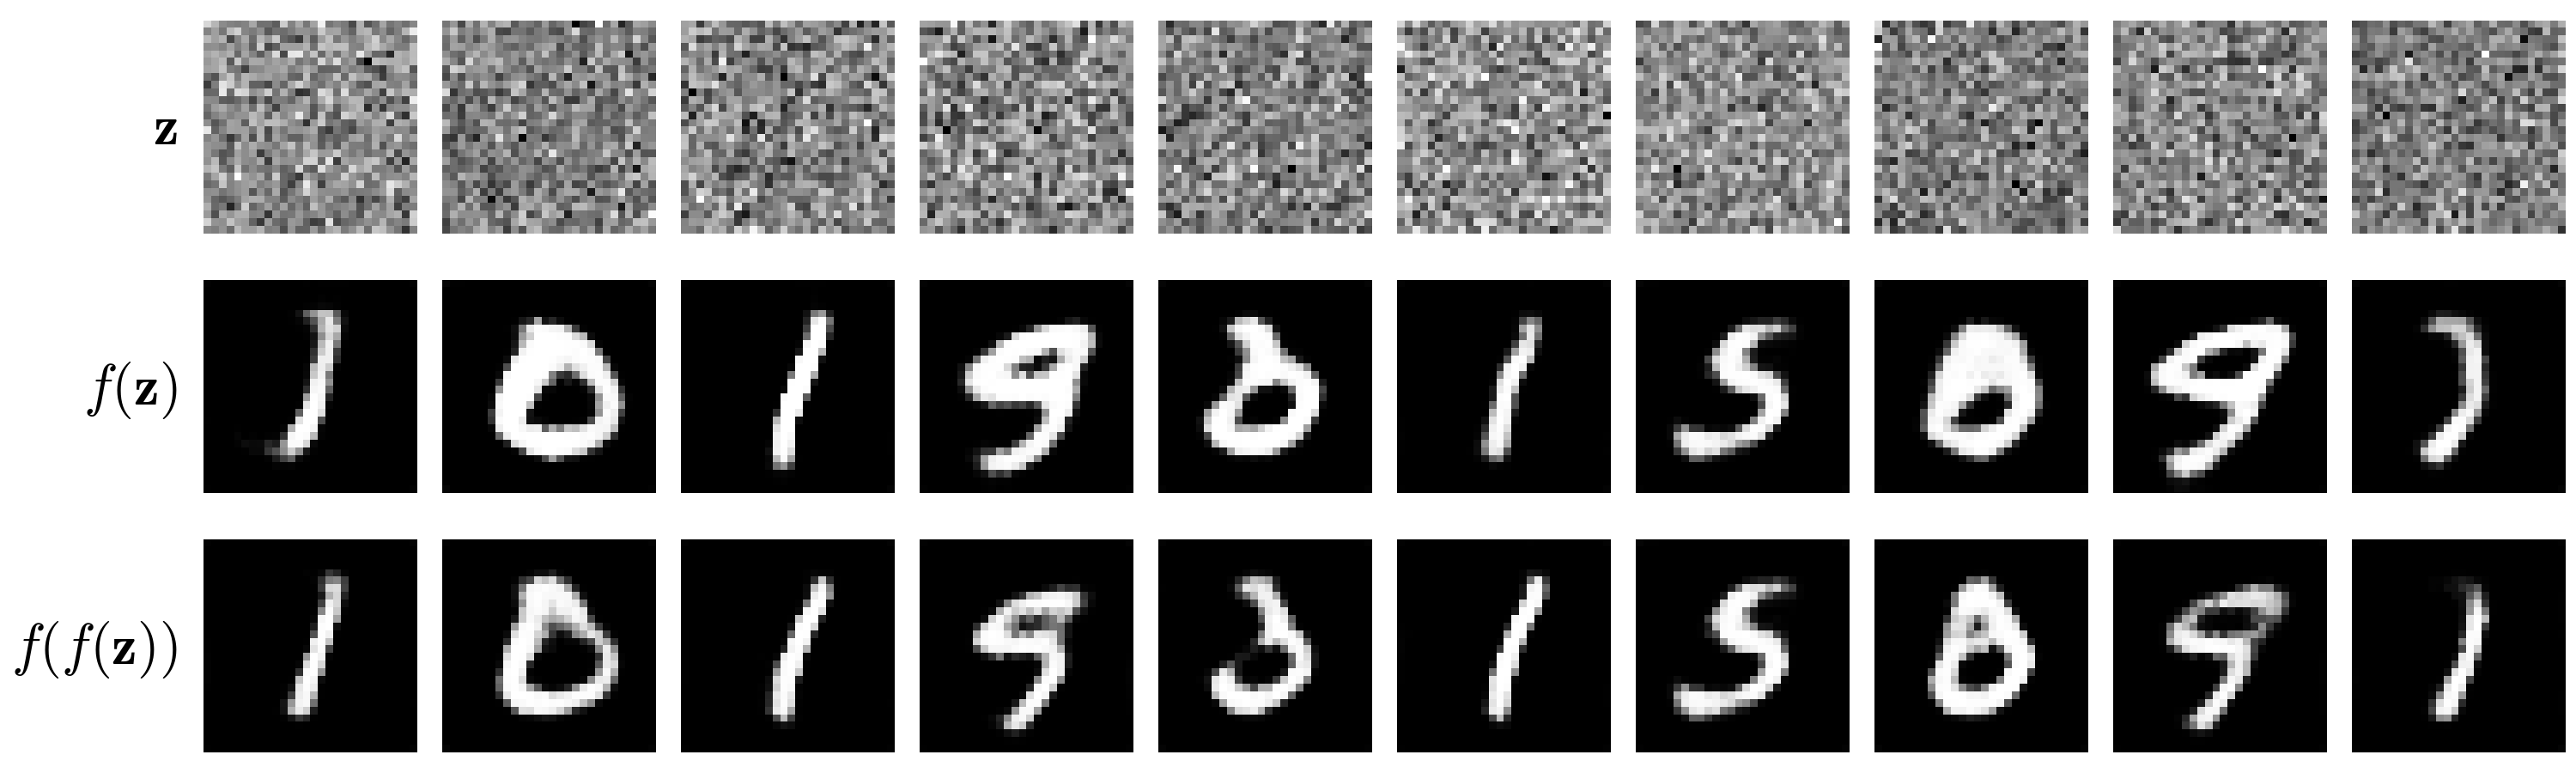
\includegraphics[width=0.7\textwidth]{./resources/modified_0-1_0-1_rand_noise_mapping.png}
    }
    \captionbox{Latent space manipulation for the U-net style DCGAN model trained on MNIST with Modified Backpropagation for optimizing idempotent and tightness losses. Samples $\mathbf{A}$ and $\mathbf{B}$ are selected randomly while remaining samples are linear combinations of these. We give the first and second application of the model.\label{fig:latent-mnist}}{
        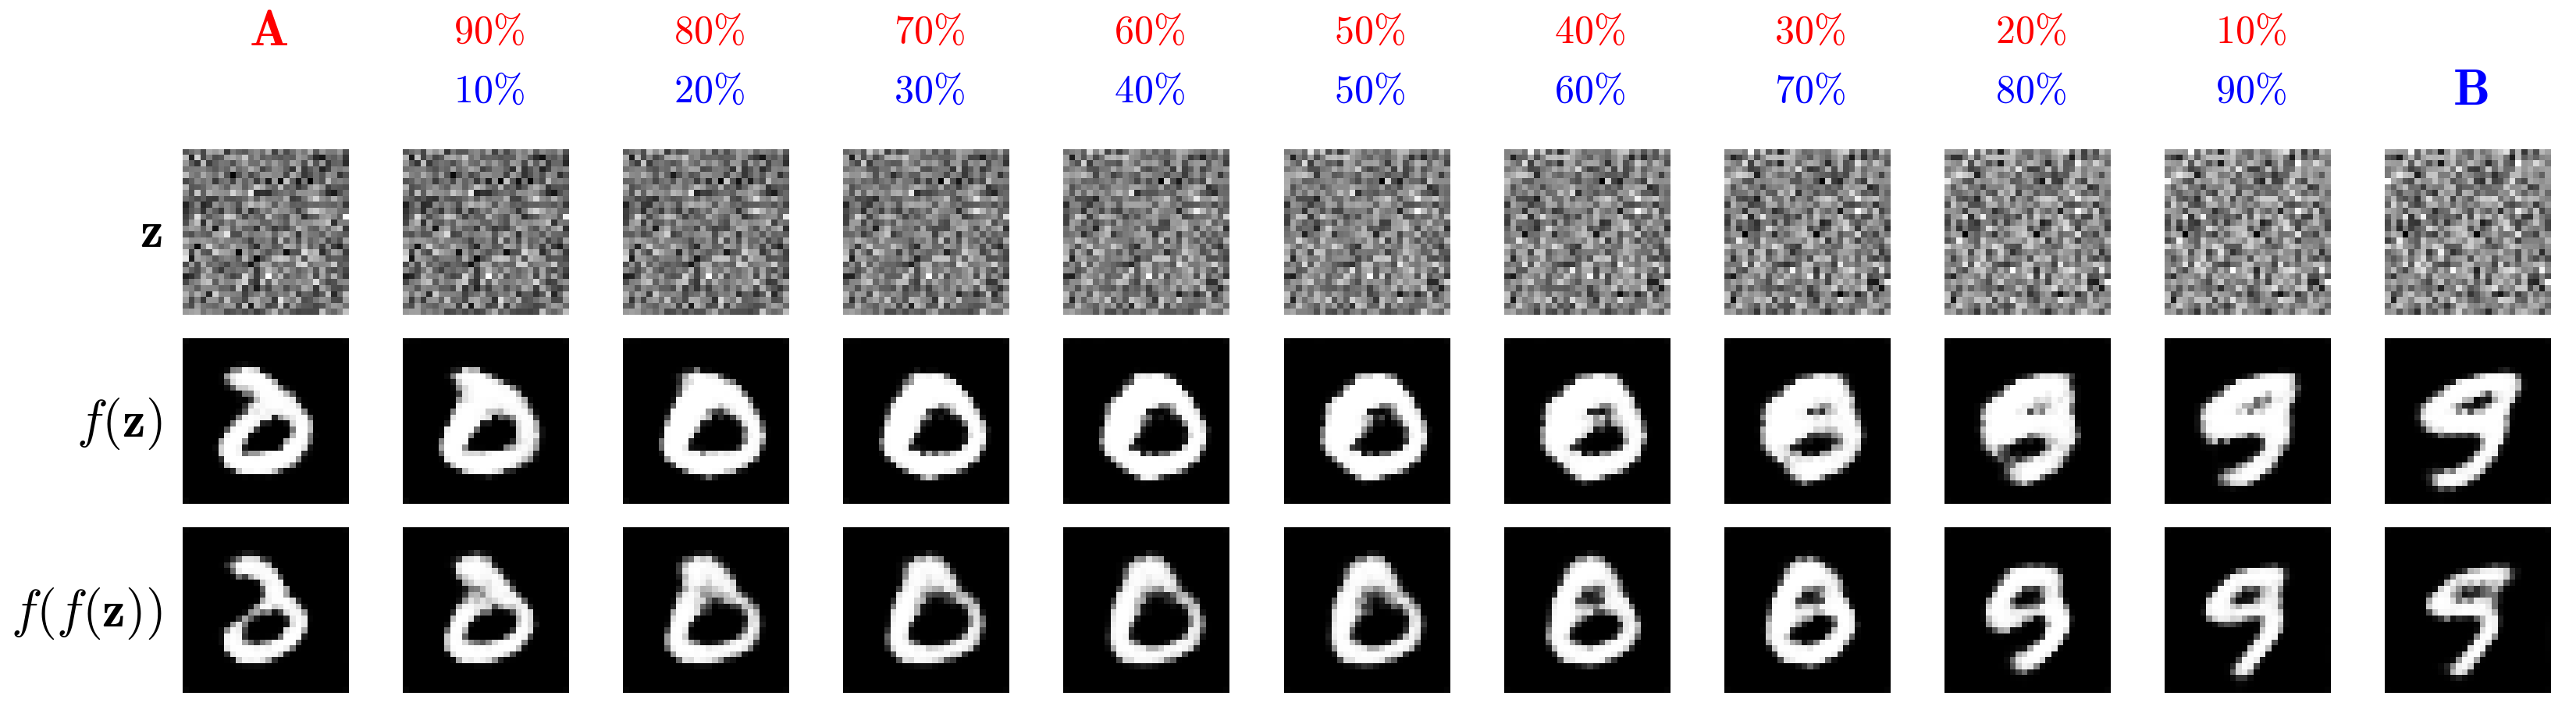
\includegraphics[width=0.8\textwidth]{./resources/modified_0-1_0-1_rand_latent_space.png}
    }
\end{figure*}

% There is future work in uncovering the relationship between the suggested gradient from MB and that of OB
\subsection{Application to Generative Networks}
\label{sec:experiment-gen}
%\textit{We replicate the results of IGN on MNIST and CelebA. Latent space analysis. Takeaway is that we show application to a U-net GAN architecture based on Conv layers.}
As mentioned, one of the motivating factors for actively enforcing idempotency during training is to apply it as a secondary optimization objective in conjunction with optimizing for a primary task. In this section we replicate the results of \citealt{shocher-ign} as we train a U-net style DCGAN architecture (see Appendix \ref{app:gen-training-scheme}) on the MNIST dataset. Let $\mathcal{D}$ denote the distribution of MNIST samples, while ${\mathcal{D}' = \mathcal{N}(0, 1)}$ from which noise is sampled. Let $\vtheta'$ is a copy of the trainable weights $\vtheta$ at each time step, where $\vtheta'$ is detached from the computational graph. In this training scheme, the loss function being optimized is
%
\begin{align}
    \begin{split}
        \mathcal{L}{(\vtheta, \vtheta')} & = \lambda_r \mathcal{L}_{\mathrm{rec}}{(\vtheta)}                                                                           \\
                                         & + \lambda_i \mathcal{L}_{\mathrm{idem}}{(\vtheta, \vtheta')} + \lambda_r \mathcal{L}_{\mathrm{tight}}{(\vtheta, \vtheta')}.
    \end{split}
    \label{eq:gan-loss}
\end{align}
%
To see why employing two copies of the weights is useful, consider $(\vx, \vy^*) \sim \mathcal{D}$ and $\vz \sim \mathcal{D}'$ and the individual loss components:
%
\begin{align}
    \mathcal{L}_{\mathrm{rec}}{((\vx, \vy^*); \vtheta)}    & = \Vert \vy^* - f_{\vtheta}(\vx) \Vert_1                            \\
    \mathcal{L}_{\mathrm{idem}}{(\vz; \vtheta, \vtheta')}  & = \Vert f_{\vtheta'}(f_{\vtheta}(\vz)) - f_{\vtheta}(\vz) \Vert_1   \\
    \mathcal{L}_{\mathrm{tight}}{(\vz; \vtheta, \vtheta')} & = -\Vert f_{\vtheta}(f_{\vtheta'}(\vz)) - f_{\vtheta'}(\vz) \Vert_1
\end{align}
%
For instance, the quantity $\pd{\mathcal{L}_{\mathrm{idem}}{(\vz; \vtheta, \vtheta')}}{\vtheta}$ is only affected by the inner application of $f$ above due to $\vtheta'$ being detached from the graph. The relationship between loss components $\mathcal{L}_{\mathrm{idem}}$ and $\mathcal{L}_{\mathrm{tight}}$ is adversarial in nature.

The major difference in this work from \citealt{shocher-ign} is that we use Modified Backpropagation for implementing both $\mathcal{L}_{\mathrm{idem}}$ and $\mathcal{L}_{\mathrm{tight}}$. As such, we effectively evaluate both loss components as the Mean Squared Error (MSE) instead of the $L_1$ loss, and we use the training scheme in Section \ref{sec:method-scheme} to construct the backwards pass (see Appendix \ref{app:gen-training-scheme}). We use the same implementation for $\mathcal{L}_{\mathrm{rec}}$ as above.

We have successfully replicated several results of \citealt{shocher-ign} under this training scheme. In particular, Figure \ref{fig:gen-mnist} shows qualitative examples of noise drawn from $\mathcal{D}'$ being mapped to images resembling samples from the MNIST dataset. While samples remains largely similar between the first and second application of the network, in some cases we do also observe the same ``self-correction'' of artefacts/noise after the second application observed by \citealt{shocher-ign}. In Figure \ref{fig:latent-mnist} we visualize the effect of applying the trained network to noise linearly interpolated between two clear samples $\vA, \vB \in \mathbb{R}^{28 \times 28}$. We again observe the secondary application of the network ``cleaning up'' images. For more uncurated examples of generated images, see Appendix \ref{app:gen-samples}.

We note that qualitative results in this training scheme for both Ordinary Backpropagation (as applied in \citealt{shocher-ign}) and Modified Backpropagation are heavily sensitive to the hyperparameters $\lambda$ chosen in Eq. (\ref{eq:gan-loss}). With fine-tuned hyperparameters we believe the results shown here are on-par with those of \citealt{shocher-ign}, whilst uncompetitive with state-of-the-art models.

% How does this fare with the one-shot inference?

Although the aim of these results is to demonstrate a practical application of Modified Backpropagation, we believe the results could be easily replicated with other datasets, such as CelebA, Cifar10, or similar. Additionally, further work is required to fully ascertain the practical benefit of Modified Backpropagation as a secondary optimization procedure in general. In particular, further experiments with other data modalities, primary optimization objectives, and datasets is needed to understand the wider applicability of the results of Sections \ref{sec:experiment-qual} and \ref{sec:experiment-quant}.

%\begin{figure*}[htbp]
%    \centering
%    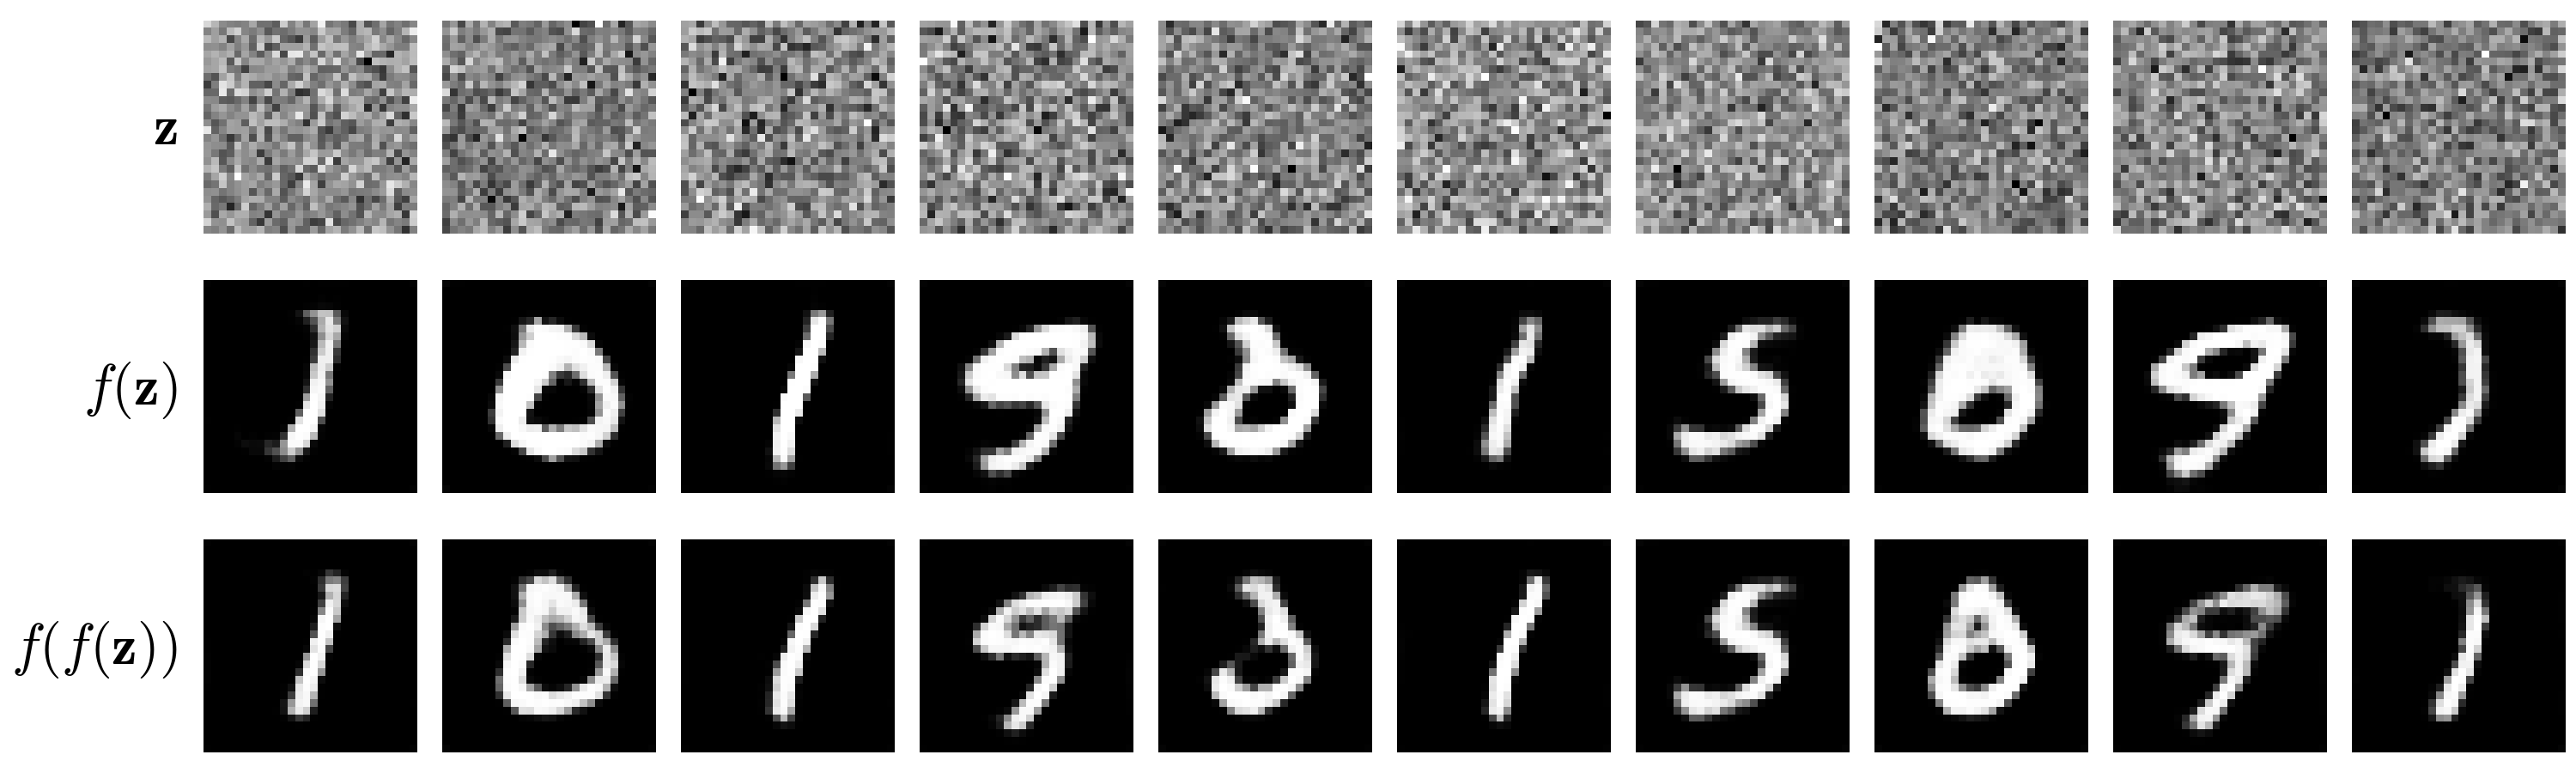
\includegraphics[width=0.7\textwidth]{./resources/modified_0-1_0-1_rand_noise_mapping.png}
%    \caption{Uncurated generations of the U-net style DCGAN model trained on MNIST with Modified %Backpropagation for optimizing idempotent and tightness losses. In the top row are samples drawn from %a random distribution with mean $0$ and variance $1$, whist the second and third rows represent first %and second application of the network to these samples, respectively.}
%    \label{fig:gen-mnist}
%\end{figure*}
%
%
%\begin{figure*}[htbp]
%    \centering
%    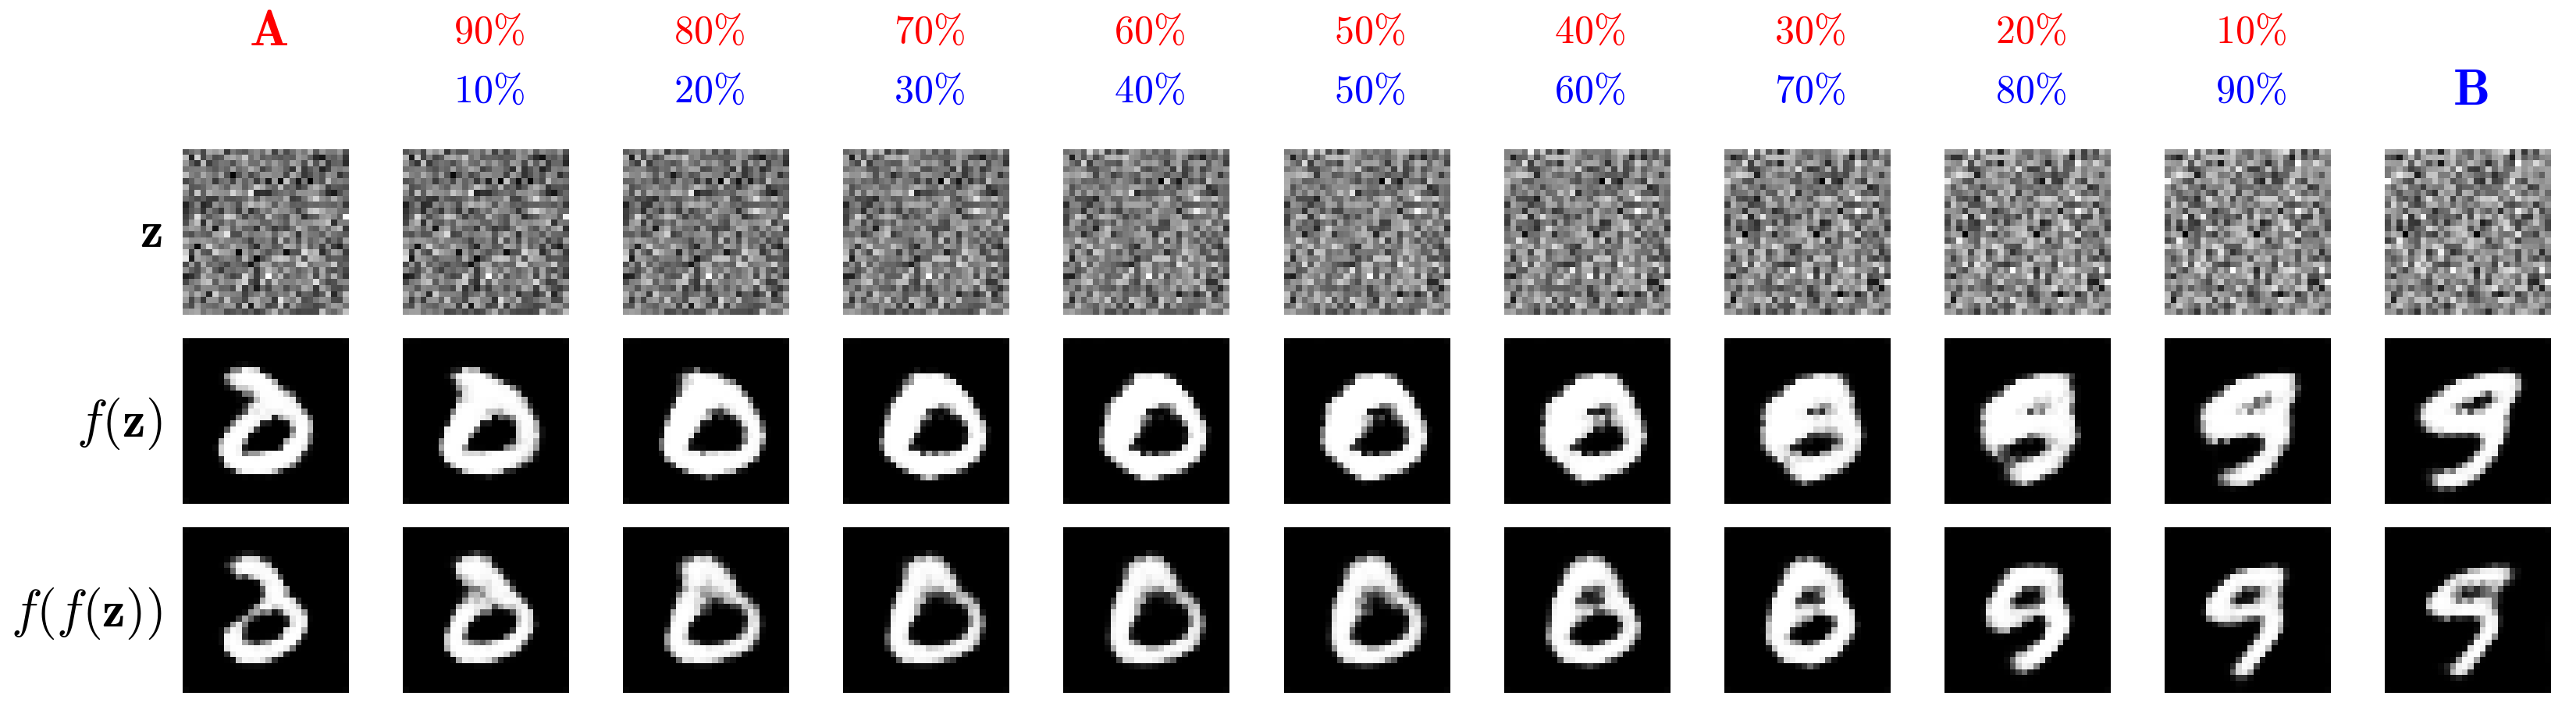
\includegraphics[width=0.8\textwidth]{./resources/modified_0-1_0-1_rand_latent_space.png}
%    \caption{Latent space manipulation for the U-net style DCGAN model trained on MNIST with Modified %Backpropagation for optimizing idempotent and tightness losses. Samples $\mathbf{A}$ and $\mathbf{B}$ %are selected randomly while remaining samples are linear combinations of these. We give the first and %second application of the model.}
%    \label{fig:latent-mnist}
%\end{figure*}

%\begin{figure}
%    \centering     %%% not \center
%    \subfigure[Modified Backpropagation]{
%        \label{fig:gen-mnist-a}
%        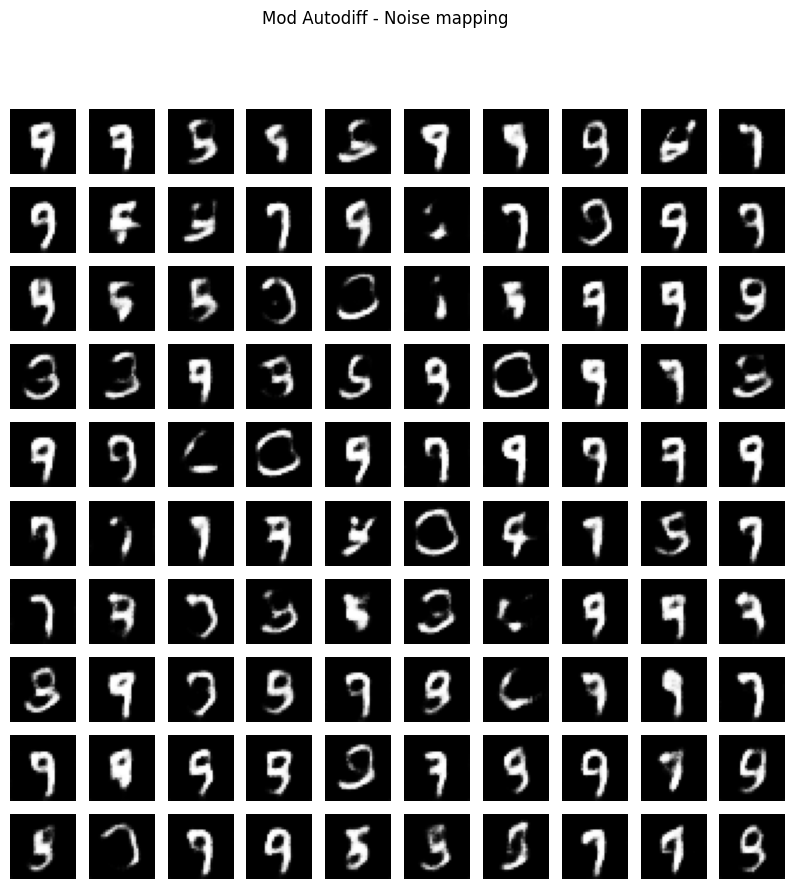
\includegraphics[width=0.9\columnwidth]{./resources/mnist-mod-autodiff-generative.png}
%    }
%    \subfigure[Ordinary Backpropagation]{
%        \label{fig:gen-mnist-b}
%        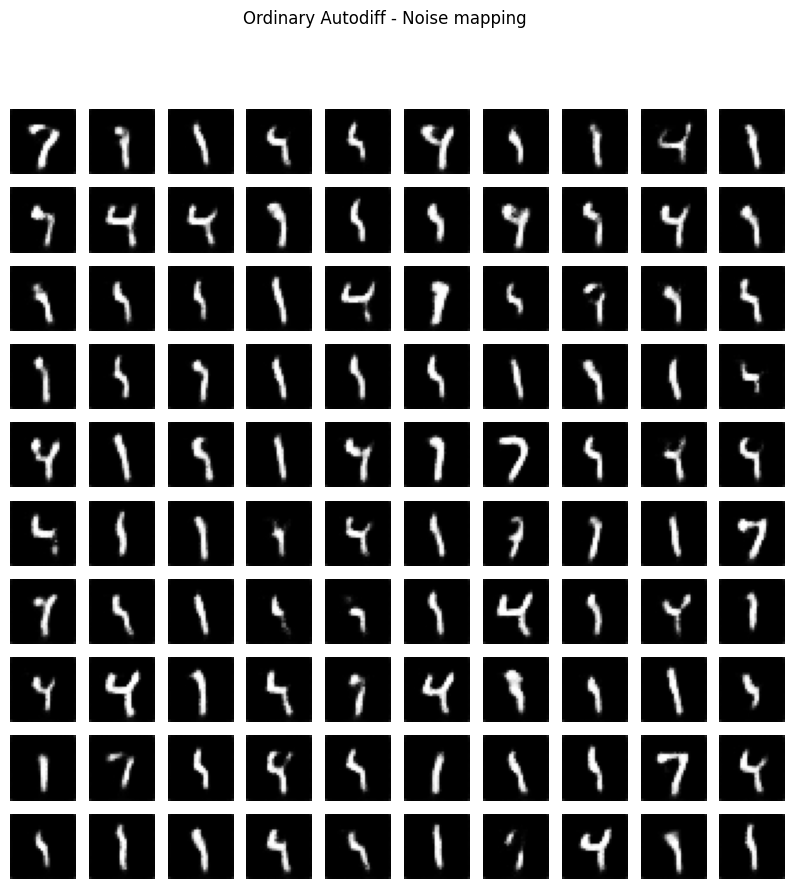
\includegraphics[width=0.9\columnwidth]{./resources/mnist-ord-autodiff-generative.png}
%    }
%    \caption{U-DCGAN architecture trained on MNIST.}
%    \label{fig:gen-mnist}
%\end{figure}


% (0.5 pages)
\section{Related Work}
\label{sec:related}
%\textit{Review Idempotent Generative Networks, contrasting our work on a gradient-free approach. Have others applied perturbation theory to ML? We suffer same problems as GANs: mode collapse.}

% IGN -> short, how is it different (grad/no-grad)
% Other optimisation strategies? check MPhil report
% Other objectives than idempotency.
% Other uses of perturbation theory in ML?

\subsection{Algebraic properties in neural networks}
There has been significant work in actively enforcing algebraic properties in weights of neural networks for a variety of reasons. For instance, in \citealt{mikolov-rnn,le-rnn-relu} it was found that enforcing \textit{part} of the weights of an RNN to remain close to the identity throughout training can cause the network to capture more long-term information, yielding performance close to LSTMs for the same natural language modelling tasks. \citealt{arjovsky-rnn} have also found that RNNs can overcome the exploding/vanishing gradient problem if weight matrices are actively enforced to be approximately unitary throughout training. Similarly, \citealt{saxe-isometry,kiani-projunn,jing-tunable-unn} all explore unitary RNNs in the same vein. Lastly, \citealt{ardizzone-inv} demonstrate that under a specialized training scheme, inverse mappings of MLPs can be found that can recover correlations in the parameter space.

These methods generally attempt to \textit{mitigate undesirable effects} inherent to particular architectures or training schemes, whereas the work we present intends to \textit{characterize behaviour} that the network should exhibit. As such, applications of the work of \citealt{shocher-ign} is closest to ours, hence we focus on this in Section \ref{sec:experiment-gen}. Nevertheless, the prolific use of orthogonal/unitary weights in the literature invites future work into adapting Modified Backpropagation to enforce orthogonality ${\big((\vK')^T(\vK')=(\vK')(\vK')^T=\vI\big)}$ as opposed to idempotency ${\big((\vK')^2 - (\vK') = \bm{0}\big)}$.


\subsection{Alternatives to gradients}
There is a large body of work focusing on approximating gradients. In \citealt{spall-perturb} a stochastic variant of finite differences called SPSA is suggested with competitive performance at lower computational cost. \citealt{scheinberg-approx,do-approx,bandler-approx} all further explore this and similar approaches based on finite differences. Nevertheless, a core idea of Modified Backpropagation is the direct substitution of the gradient of $\mathcal{L}_{\mathrm{idem}}$ with the quantity in Eq. (\ref{eq:substitution}). Although the exact relationship between this quantity and the gradients produced by Ordinary Backpropagation is still unclear, it is certainly not a direct approximation as evidenced in Section \ref{sec:experiment-qual}.


% (0.5 pages)
\section{Conclusion}
\label{sec:conclusion}
%\textit{Give a conclusion of central idea: the use of perturbation analysis to find an iterator which we have successfully applied to a range of toy examples and GAN scenarios.}
In this work, we have given motivation for actively enforcing idempotency in arbitrary neural networks used in data transformation. The central idea presented is the idempotent corrector ${g(\vK) = 3\vK^3 - 2\vK^2}$, which has been derived by solving a linear program such that ${\vK' = g(\vK)}$ for a near-idempotent matrix $\vK$ and a perfectly idempotent $\vK'$. We have also expanded the idea to a training scheme for arbitrary neural networks via a small modification to the canonical backpropagation algorithm, termed Modified Backpropagation. Experimental results have shown that optimizer trajectories generally differ from those of Ordinary Backpropagation across a wide variety of MLP network configurations. Furthermore, we showed that Modified Backpropagation outperforms Ordinary Backpropagation in finding neural networks with lower idempotent error by up to an order of magnitude. Lastly, we demonstrate that Modified Backpropagation can be used alongside Ordinary Backpropagation to train generative models on MNIST, following the example of \citealt{shocher-ign}.

We believe the work presented here suggests that alternative methods to gradient-based optimization in neural networks are practically viable, and we hope that future work will explore other applications of the central ideas presented here.

% Acknowledgements should only appear in the accepted version.
%\section*{Acknowledgements}
%
%\textbf{Do not} include acknowledgements in the initial version of
%the paper submitted for blind review.
%
%If a paper is accepted, the final camera-ready version can (and
%usually should) include acknowledgements.  Such acknowledgements
%should be placed at the end of the section, in an unnumbered section
%that does not count towards the paper page limit. Typically, this will
%include thanks to reviewers who gave useful comments, to colleagues
%who contributed to the ideas, and to funding agencies and corporate
%sponsors that provided financial support.

\section*{Impact Statement}
This paper presents work whose goal is to advance the field of
Machine Learning. There are many potential societal consequences
of our work, none which we feel must be specifically highlighted here.

%Authors are \textbf{required} to include a statement of the potential broader impact of their work, including its ethical aspects and future societal consequences. This statement should be in an unnumbered section at the end of the paper (co-located with Acknowledgements -- the two may appear in either order, but both must be before References), and does not count toward the paper page limit. In many cases, where the ethical impacts and expected societal implications are those that are well established when advancing the field of Machine Learning, substantial discussion is not required, and a simple statement such as the following will suffice:

%``This paper presents work whose goal is to advance the field of Machine Learning. There are many potential societal consequences of our work, none which we feel must be specifically highlighted here.''

%The above statement can be used verbatim in such cases, but we encourage authors to think about whether there is content which does warrant further discussion, as this statement will be apparent if the paper is later flagged for ethics review.


% In the unusual situation where you want a paper to appear in the
% references without citing it in the main text, use \nocite
%\nocite{langley00}

\bibliography{bibliography}
\bibliographystyle{icml2025}


%%%%%%%%%%%%%%%%%%%%%%%%%%%%%%%%%%%%%%%%%%%%%%%%%%%%%%%%%%%%%%%%%%%%%%%%%%%%%%%
%%%%%%%%%%%%%%%%%%%%%%%%%%%%%%%%%%%%%%%%%%%%%%%%%%%%%%%%%%%%%%%%%%%%%%%%%%%%%%%
% APPENDIX
%%%%%%%%%%%%%%%%%%%%%%%%%%%%%%%%%%%%%%%%%%%%%%%%%%%%%%%%%%%%%%%%%%%%%%%%%%%%%%%
%%%%%%%%%%%%%%%%%%%%%%%%%%%%%%%%%%%%%%%%%%%%%%%%%%%%%%%%%%%%%%%%%%%%%%%%%%%%%%%
\newpage
\appendix
\onecolumn

\section{Solutions to the ansatz}
\label{app:solutions}
We give a detailed description of how to derive idempotent operators for $\vK$ that are near-idempotent to order $n$ with a fixed dimension $j$. For a given $j$, find a mapping $g$ making the input idempotent:
\begin{enumerate}
    \item Assume $\vK = \vP + \vD$.
    \item {Assume that $\vD^2 \approx \bm{0}$, $\vP^2 = \vP$, and $\vX \vD \vY \vD \vZ \approx \bm{0} \mathrm{~for~all~} \vX,\vY,\vZ$.}
    \item {Expand the expression $(\vK')^2 - \vK' = 0$.
          \begin{itemize}
              \item $j = 2$ gives 34 terms
              \item $j = 3$ gives 154 terms
              \item $j = 6$ gives 10,794 terms
          \end{itemize}
          }
    \item {Apply assumptions from 2 recursively.
          \begin{itemize}
              \item $j = 2$ reduces 34 to \textbf{16 terms}
              \item $j = 3$ reduces 154 to \textbf{32 terms}
              \item $j = 6$ reduces 10,794 to \textbf{104 terms}
          \end{itemize}
          }
    \item Collect coefficients for $\vD$, $\vP$, $\vD\vP$, $\vP\vD$, and $\vP\vD\vP$ (no other exist).
    \item Create a set of equations from coefficients and solve as a linear program.
\end{enumerate}

For $n=1$ we give the first $j=1,\dots, 8$ idempotent correctors:
\begin{itemize}
    \item For $j=1, 2$, there are no solutions.
    \item {For $j=3$, there is one solution (found in $\sim130$ ms):
          \begin{align}
              g(\vK) = 3 \vK^2 - 2 \vK^3
          \end{align}
          }
    \item {For $j=4$, there is a family of solutions (found in $\sim620$ ms):
          \begin{align}
              g(\vK) = \frac{4 - \alpha_3}{2} \vK^2 + \alpha_3 \vK^3 - \frac{2 + \alpha_3}{2} \vK^4
          \end{align}
          }
    \item {For $j=5$, there is a family of solutions (found in $\sim3.8$ s):
          \begin{align}
              g(\vK) = \frac{4 - \alpha_3 + \alpha_5}{2} \vK^2 + \alpha_3 \vK^3 - \frac{2 + \alpha_3 + 3\alpha_5}{2} \vK^4 + \alpha_5  \vK^5
          \end{align}
          }
    \item {For $j=6$, there is a family of solutions (found in $\sim24$ s):
          \begin{align}
              g(\vK) = \frac{6 - 3\alpha_3 - 2\alpha_4 - \alpha_5}{4} \vK^2 + \alpha_3 \vK^3 + \alpha_4 \vK^4 + \alpha_5  \vK^5 - \frac{2 + \alpha_3 + 2\alpha_4 + 3 \alpha_5}{4} \vK^6
          \end{align}
          }
    \item {For $j=7$, there is a family of solutions (found in $\sim152$ seconds):
          \begin{align}
              \begin{split}
                  g(\vK) = & \frac{7 - 4\alpha_3 - 3 \alpha_4 - 2\alpha_5 - \alpha_6}{5} \vK^2 + \alpha_3 \vK^3 + \alpha_4 \vK^4     \\
                           & + \alpha_5  \vK^5 + \alpha_6 \vK^6 - \frac{2 + \alpha_3 + 2\alpha_4 + 3 \alpha_5 + 4 \alpha_6}{5} \vK^7
              \end{split}
          \end{align}
          }
    \item {For $j=8$, there is a family of solutions (found in $\sim922$ seconds):
          \begin{align}
              \begin{split}
                  g(\vK) = & \frac{8 - 5\alpha_3 - 4 \alpha_4 - 3\alpha_5 - 2\alpha_6 - \alpha_7}{6} \vK^2 + \alpha_3 \vK^3 + \alpha_4 \vK^4                      \\
                           & + \alpha_5  \vK^5 + \alpha_6 \vK^6 + \alpha_7 \vK^7 - \frac{2 + \alpha_3 + 2\alpha_4 + 3 \alpha_5 + 4\alpha_6 + 5 \alpha_7}{6} \vK^8
              \end{split}
          \end{align}
          }

\end{itemize}

\newpage
\section{Jordan normal form analysis}
\label{app:jordan}
Let ${d_\lambda = \alpha(\lambda)}$ denote the algebraic multiplicity of eigenvalue $\lambda$ and let $\gamma(\lambda)$ denote the geometric multiplicity of $\lambda$. Given the equation
\begin{equation}
    \vK = 3\vK^2 - 2\vK^3,
    \label{eq:k-problem}
\end{equation}
we can substitute $\vK = \vP\vJ\vP^{-1}$,
\begin{equation}
    \vP\vJ\vP^{-1} = 3(\vP\vJ\vP^{-1})^2 - 2(\vP\vJ\vP^{-1})^3,
\end{equation}
which can be simplified to
\begin{equation}
    \vP\vJ\vP^{-1} = 3\vP\vJ^2\vP^{-1} - 2\vP\vJ^3\vP^{-1}.
\end{equation}

Since $\vP$ is invertible, this is equivalent to:
\begin{equation}
    \vJ = 3\vJ^2 - 2\vJ^3.
    \label{eq:j-problem}
\end{equation}

Thus for an arbitrary $\vK$, solving Eq. (\ref{eq:k-problem}) equates to solving Eq. (\ref{eq:j-problem}).

Since $\vJ$ is block-diagonal, the equation in (\ref{eq:j-problem}) can be broken down into smaller equations for each block, ${\vJ_{\lambda} = 3\vJ_{\lambda}^2 - 2\vJ_{\lambda}^3}$, which we can write as a system of equations:
\begin{equation}
    \begin{pmatrix}
        \lambda & 1       & 0       & \hdots & 0       \\
        0       & \lambda & 1       & \hdots & 0       \\
        0       & 0       & \lambda & \hdots & 0       \\
        \vdots  & \vdots  & \vdots  & \ddots & \vdots  \\
        0       & 0       & 0       & \hdots & \lambda \\
    \end{pmatrix} = 3\begin{pmatrix}
        \lambda^2 & 2\lambda  & 1         & \hdots & 0         \\
        0         & \lambda^2 & 2\lambda  & \hdots & 0         \\
        0         & 0         & \lambda^2 & \hdots & 0         \\
        \vdots    & \vdots    & \vdots    & \ddots & \vdots    \\
        0         & 0         & 0         & \hdots & \lambda^2 \\
    \end{pmatrix} - 2\begin{pmatrix}
        \lambda^3 & 3\lambda^2 & 3\lambda   & 1          & \hdots & 0         \\
        0         & \lambda^3  & 3\lambda^2 & 3\lambda   & \hdots & 0         \\
        0         & 0          & \lambda^3  & 3\lambda^2 & \hdots & 0         \\
        \vdots    & \vdots     & \vdots     & \vdots     & \ddots & \vdots    \\
        0         & 0          & 0          & 0          & \hdots & \lambda^3 \\
    \end{pmatrix}
\end{equation}

Thus, for a ${(d_\lambda \times d_\lambda)}$ Jordan block we have up to four equations per eigenvalue:
\begin{align}
    \lambda & = 3\lambda^2 - 2\lambda^3                             & \label{eq:app-cond1}                                    \\
    1       & = 3(2\lambda) - 2(3\lambda^2) = 6\lambda - 6\lambda^2 & \text{Only when $d_\lambda \geq2$.}\label{eq:app-cond2} \\
    0       & = 3(1) - 2(3\lambda) = 3 - 6\lambda                   & \text{Only when $d_\lambda \geq3$.}\label{eq:app-cond3} \\
    0       & = 3(0) - 2(1) = 0 - 2                                 & \text{Only when $d_\lambda \geq4$.}\label{eq:app-cond4}
\end{align}
There are never more equations than this, since all other entries in a Jordan block must be 0.

Since Eq. (\ref{eq:app-cond4}) is a contradiction, we can have no solution which solves all Eqs. (\ref{eq:app-cond1}), (\ref{eq:app-cond2}), (\ref{eq:app-cond3}), and (\ref{eq:app-cond4}). Note also that there exists no solutions satisfying Eqs. (\ref{eq:app-cond1}), (\ref{eq:app-cond2}), and (\ref{eq:app-cond3}), nor do any solutions exist for both Eqs. (\ref{eq:app-cond1}) and (\ref{eq:app-cond2}). The following are solutions which satisfy only Eq. (\ref{eq:app-cond1}):
\begin{equation}
    \lambda =\{0, 0.5, 1\}
\end{equation}

The only situation where Eqs. (\ref{eq:app-cond2}), (\ref{eq:app-cond3}), and (\ref{eq:app-cond4}) do not arise is when ${\alpha(\lambda)=\gamma(\lambda)}$, which is precisely the case when $\vK$ is diagonalizable. Therefore, any $\vK$ which is a solution to (\ref{eq:k-problem}) must have a Jordan normal form which is a diagonal matrix:
\begin{equation}
    \vJ = \begin{pmatrix}
        \lambda_1 & 0         & 0      & \hdots & 0         \\
        0         & \lambda_2 & 0      & \hdots & 0         \\
        \vdots    & \vdots    & \vdots & \ddots & \vdots    \\
        0         & 0         & 0      & \hdots & \lambda_3 \\
    \end{pmatrix}
\end{equation}

%We can therefore arrive at the following conclusions:
%\begin{itemize}
%    \item $\vK$ must be diagonalizable.
%    \item $\vK$ cannot have complex eigenvalues (they must be from the set $\{0, 0.5, 1\}$).
%    \item All idempotent matrices are possible choices for $\vK$. A matrix $\vA$ is idempotent if and only if all its %eigenvalues are either 0 or 1.
%    \item {There are non-idempotent matrices which are choices for $\vK$. Any matrix with $0.5$ as an eigenvalue (and possibly %any other eigenvalues) will be a fixed point, but it will not be idempotent. This is an example:
%          \begin{equation*}
%              \vA = \begin{pmatrix}
%                  0.5 & 0 \\
%                  0   & 1
%              \end{pmatrix}
%          \end{equation*}
%          }
%\end{itemize}

\newpage
\section{Automatic differentiation rule}
\label{app:autodiff-rule}
To implement Modified Backpropagation in PyTorch we make use of custom autograd functions. The mathematical description of the loss function for idempotency is:
%
\begin{align}
    \mathcal{L}_{\mathrm{idem}}(\vy) = \frac{1}{n} \sum_{i = 1}^n \left( f_{\vtheta}(\vy) - \vy \right)^2.
\end{align}

To practically implement the function, we note that PyTorch optimizers reduce $-\mathcal{L}$ for some loss function $\mathcal{L}$, but as per Section \ref{sec:method} our method reduces idempotent when the loss function above is \textit{not} negatively signed. This leads to the implementation in \texttt{E.backward} function in algorithm \ref{alg:rule}.

\begin{algorithm}[htbp]
    \caption{Modified Backpropagation PyTorch rule.}
    \label{alg:rule}
    \begin{python}
class E(torch.autograd.Function):
    @staticmethod
    def loss_fn(y, net):
        loss = torch.mean((net(y) - y) ** 2)
        return loss

    @staticmethod
    def forward(ctx, y, net):
        ctx.save_for_backward(y)
        ctx.net = net

        return E.loss_fn(y, net)

    @staticmethod
    def backward(ctx, grad_output):
        y, = ctx.saved_tensors
        net = ctx.net

        y2 = net(y)
        y3 = net(y2)
        e = 3*y2 - 2*y3 - y
        grads = -e / e.shape[0]
        return grads * grad_output, None

class ELoss(torch.nn.Module):
    def __init__(self, net, mode):
        super(ELoss, self).__init__()
        self.net = net
        self.mode = mode

    def forward(self, y):
        return E.apply(y, self.net)
\end{python}
\end{algorithm}

\clearpage

We give the computational graph constructed by PyTorch for calculating gradients in Modified Backpropagation and Ordinary Backpropagation. The graphs are constructed using the same single-layer neural network without biases and no activation function. We therefore have ${f_{\vtheta}(\vx)=\vW\vx}$. \textbf{PyTorch, however, represents the input $\vx$ transposed, hence the following use  ${f_{\vtheta}(\vx)=\vW\vx^T=\vx\vW^T}$ as the definition.} We show the graphs describing the computation of gradients for $\vW$ for a single optimization step.

In these graphs, the weight matrix $\vW$ is the blue box, and the green box at the bottom of the graph is the gradient matrix $\pd{\mathcal{L}_{\mathrm{idem}}(f_{\vtheta}(\vx))}{\vW}$. Yellow boxes of size $3 \times 5$ denote the input $\vx$ consisting of 3 samples with 5 features each.

\begin{figure}[H]
    \centering
    \subfigure[\textbf{Modified Backpropagation}]{
        \label{fig:mod_autodiff_graph}
        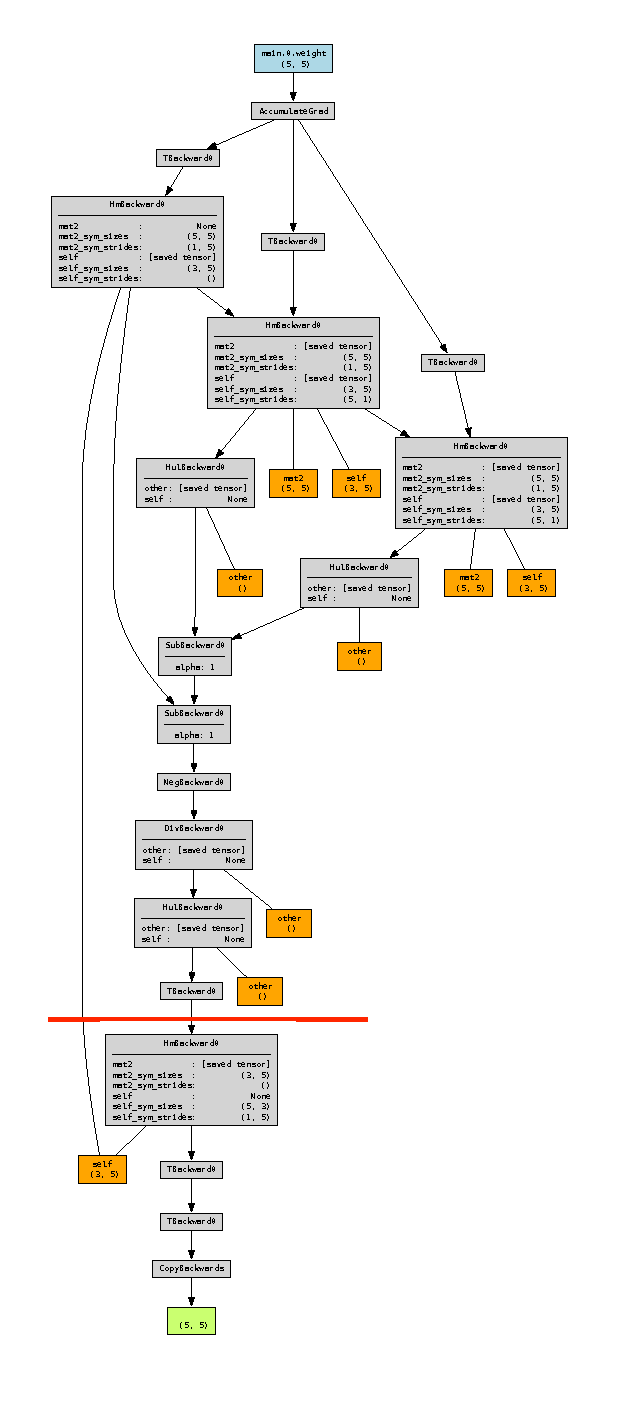
\includegraphics[width=.33\linewidth]{resources/comp_graph_mod_autodiff.pdf}
    }
    \subfigure[\textbf{Ordinary Backpropagation}]{
        \label{fig:ord_autodiff_graph}
        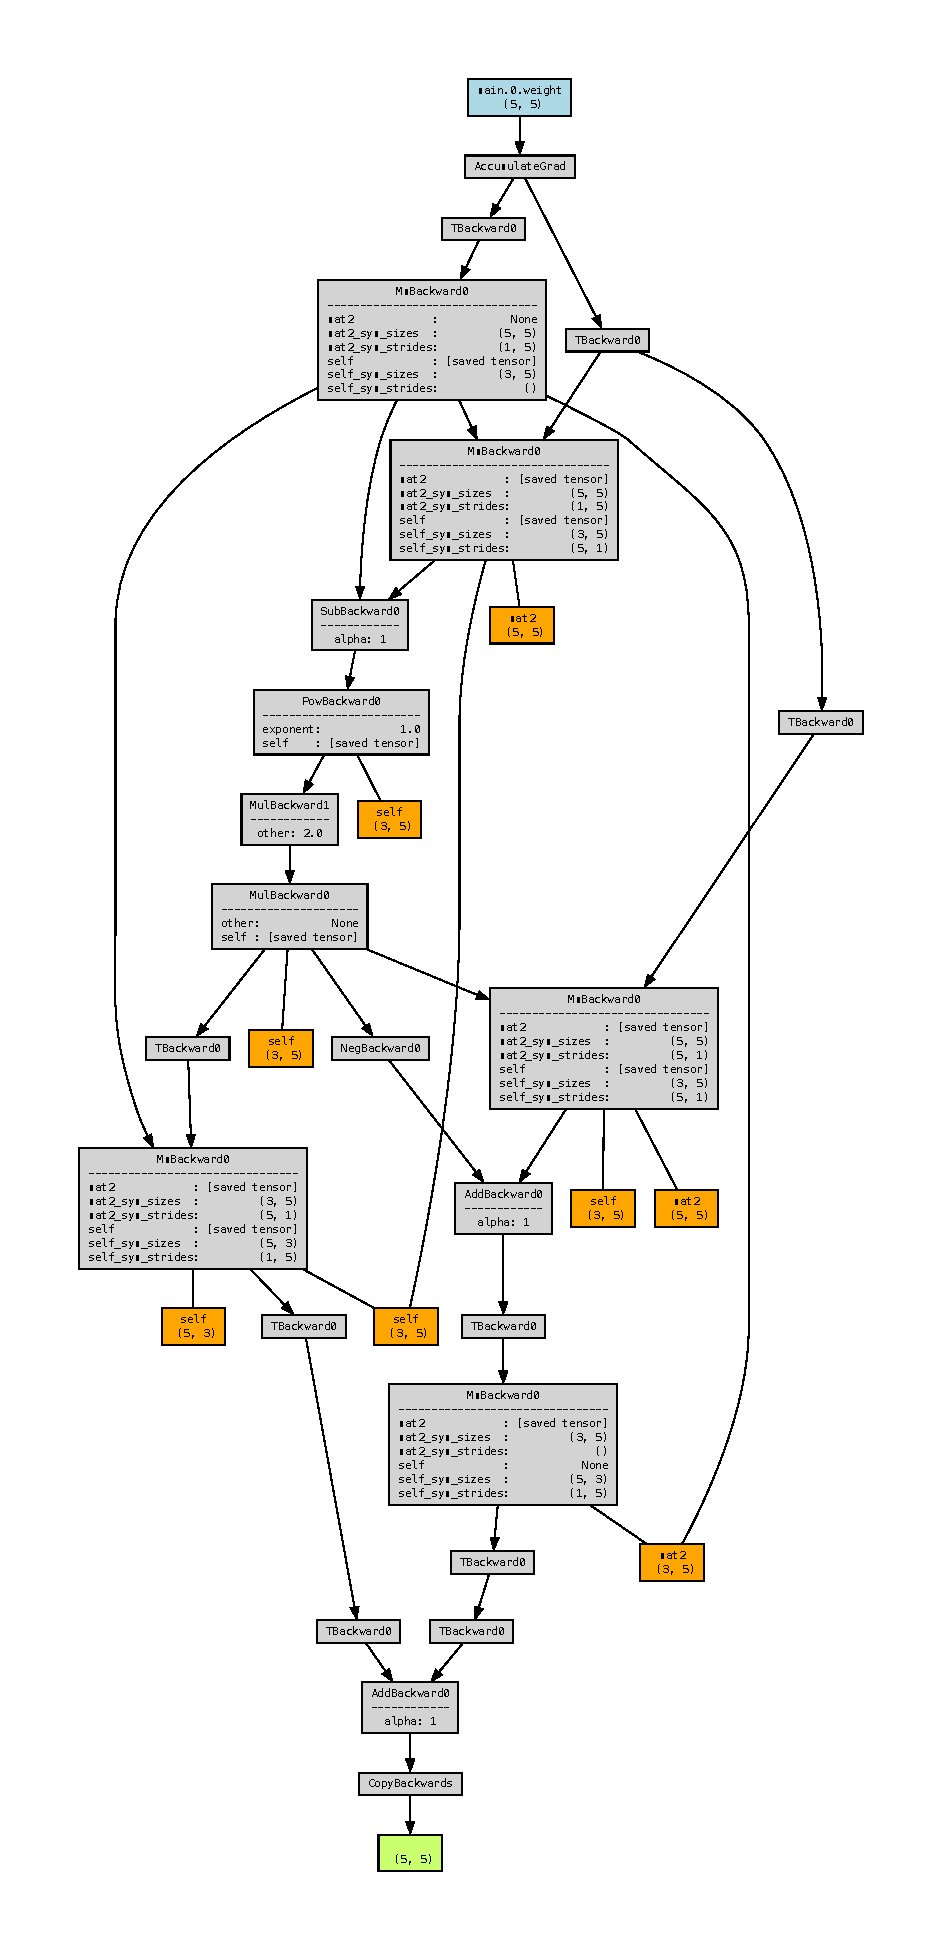
\includegraphics[width=.33\linewidth]{resources/comp_graph_ord_autodiff.pdf}
    }
    \caption{PyTorch computational graphs for gradient calculation.}
    \label{fig:comp-graphs}
\end{figure}

The red line in Figure \ref{fig:mod_autodiff_graph} denotes the intuitive split by the chain rule. Computation above the line corresponds to $\pd{\mathcal{L}_{\mathrm{idem}}(\vy)}{\vy}$ and computation below the line corresponds to $\pd{f_{\vtheta}(\vx)}{\vW}$, which altogether gives $\pd{\mathcal{L}_{\mathrm{idem}}(f_{\vtheta}(\vx))}{\vW}$. Chasing through the graph shows that it indeed does use exactly the algorithm outlined above.

The graph in Figure \ref{fig:ord_autodiff_graph} shows a computation of $\pd{\mathcal{L}_{\mathrm{idem}}(f_{\vtheta}(\vx))}{\vW}$ without using \pyth{E.backward}. Although the graph is less obvious, chasing the graph shows that it computes the following quantity:
%
\begin{align*}
    (2(\vx\vW^T\vW^T-\vx\vW^T) \cdot \vx)^T \vx\vW^T + ((2(\vx\vW^T\vW^T-\vx\vW^T) \cdot \vx) \vW - 2(\vx\vW^T\vW^T-\vx\vW^T) \cdot \vx)^T \vx.
\end{align*}
%
This is equivalent to the ordinary analytical solution to $\pd{\mathcal{L}_{\mathrm{idem}}(f_{\vtheta}(\vx))}{\vW}$.

\newpage
\section{Test networks error and norm}
\label{app:test-networks-data}

For each of the test networks outlined in table \ref{tab:networks} we report the distribution of absolute idempotent error and norm of the resulting mapping in Figures \ref{fig:error-test-nets} and \ref{fig:norm-test-nets}. The learning rates used for training of each network is chosen to be the value in Figure \ref{fig:avg-abs-err} with the lowest idempotent error for each algorithm and network configuration.

\begin{figure}[H]
    \centering
    \subfigure[Network B1]{
        \label{fig:error-test-nets-1}
        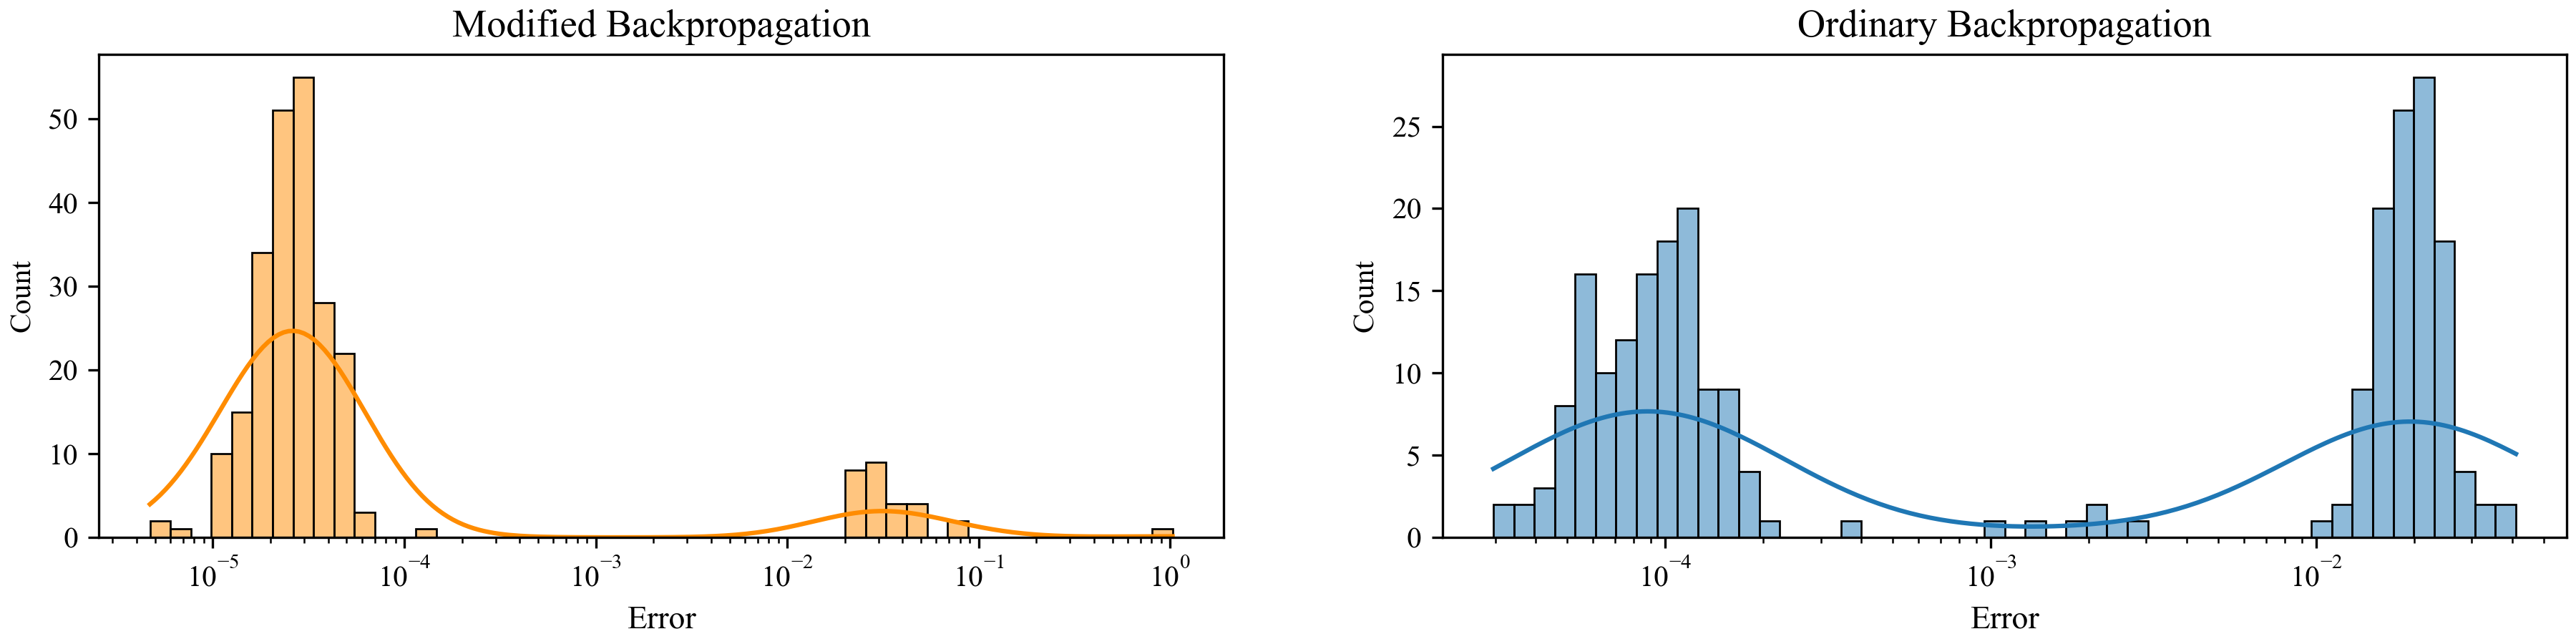
\includegraphics[width=.9\linewidth]{resources/hist_abs_err_b1.png}
    }
    \subfigure[Network B2]{
        \label{fig:error-test-nets-2}
        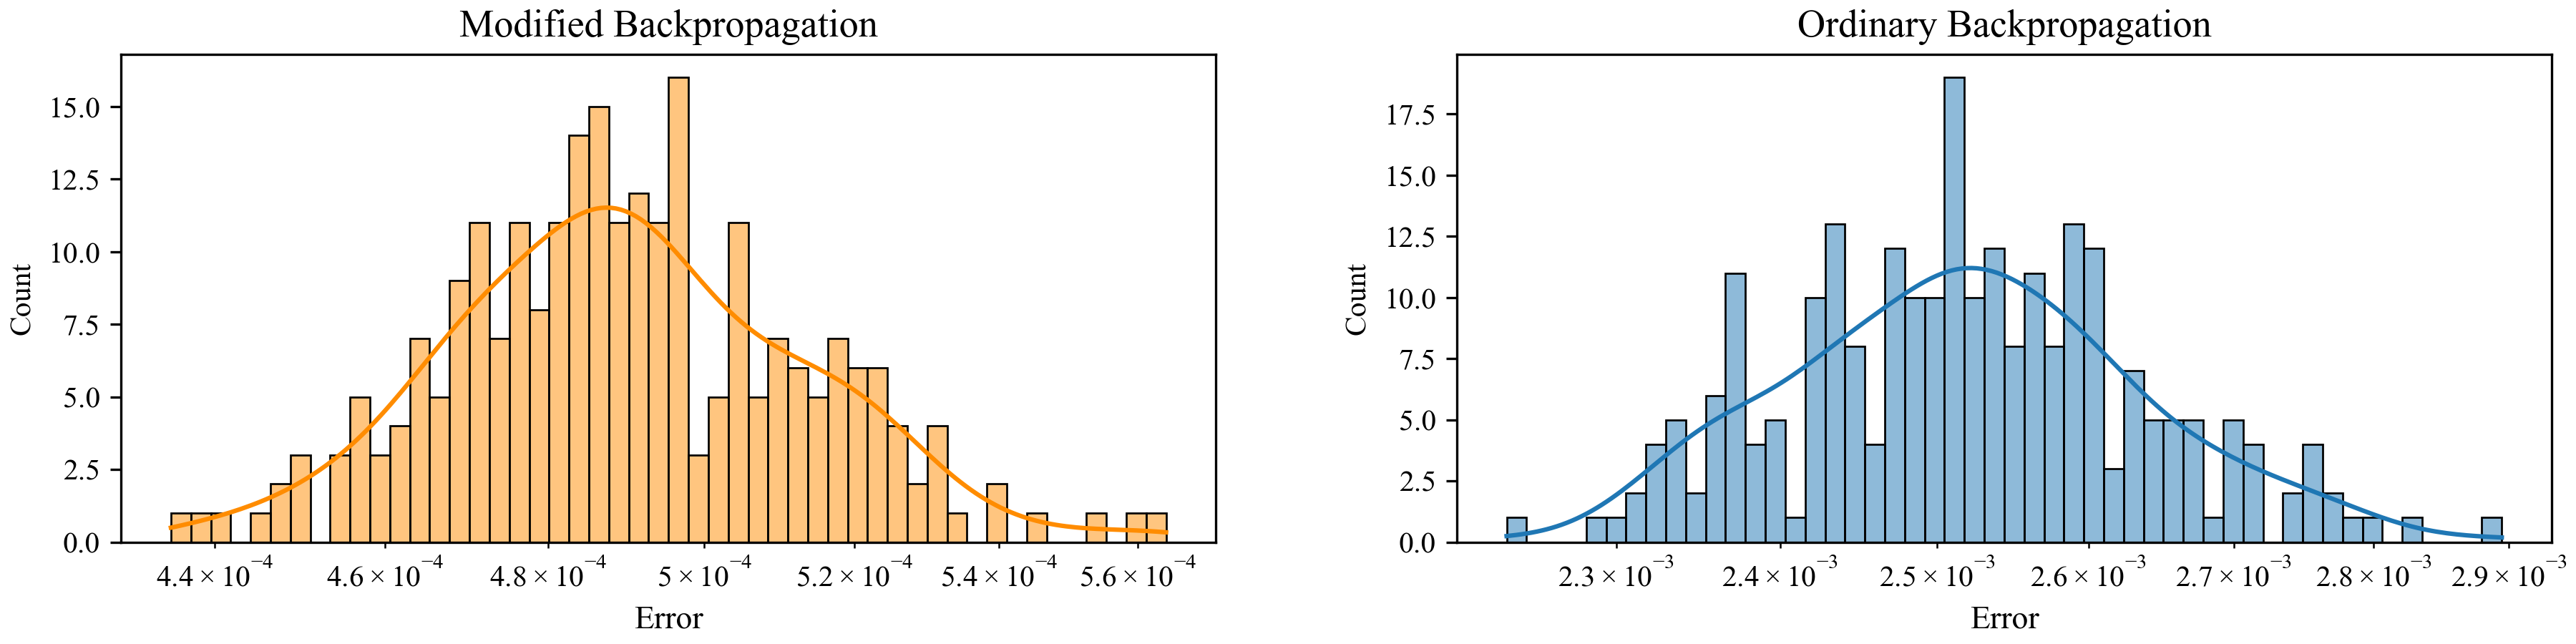
\includegraphics[width=.9\linewidth]{resources/hist_abs_err_b2.png}
    }
    \subfigure[Network B3]{
        \label{fig:error-test-nets-3}
        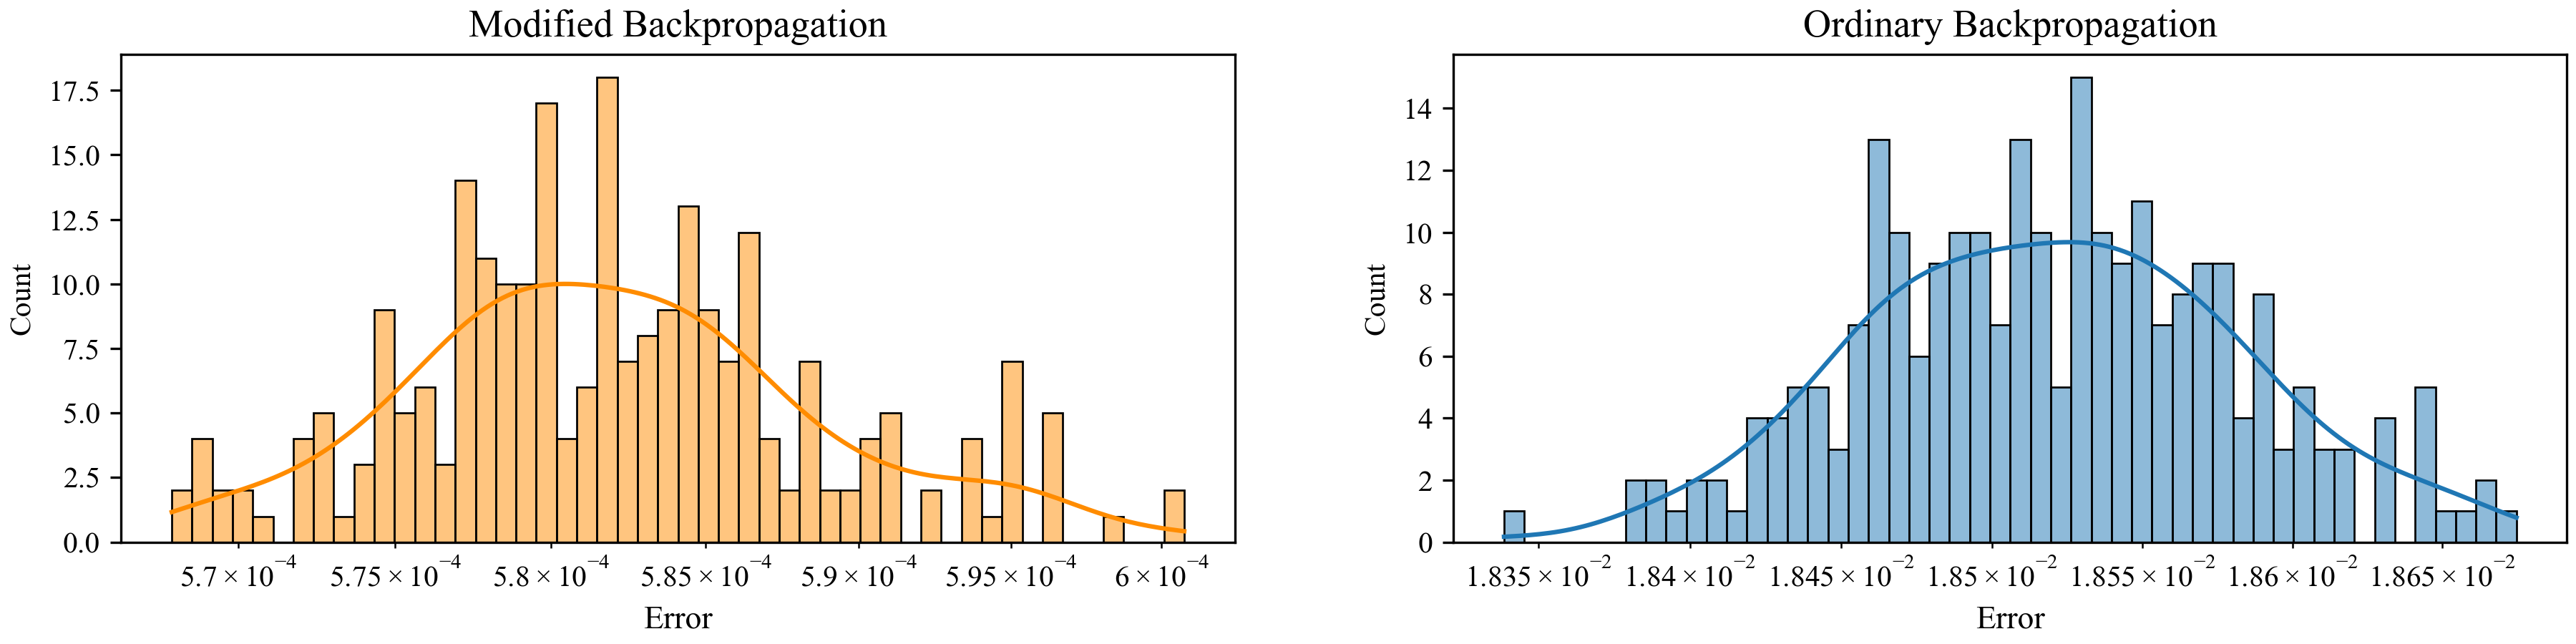
\includegraphics[width=.9\linewidth]{resources/hist_abs_err_b3.png}
    }
    \subfigure[Network B4]{
        \label{fig:error-test-nets-4}
        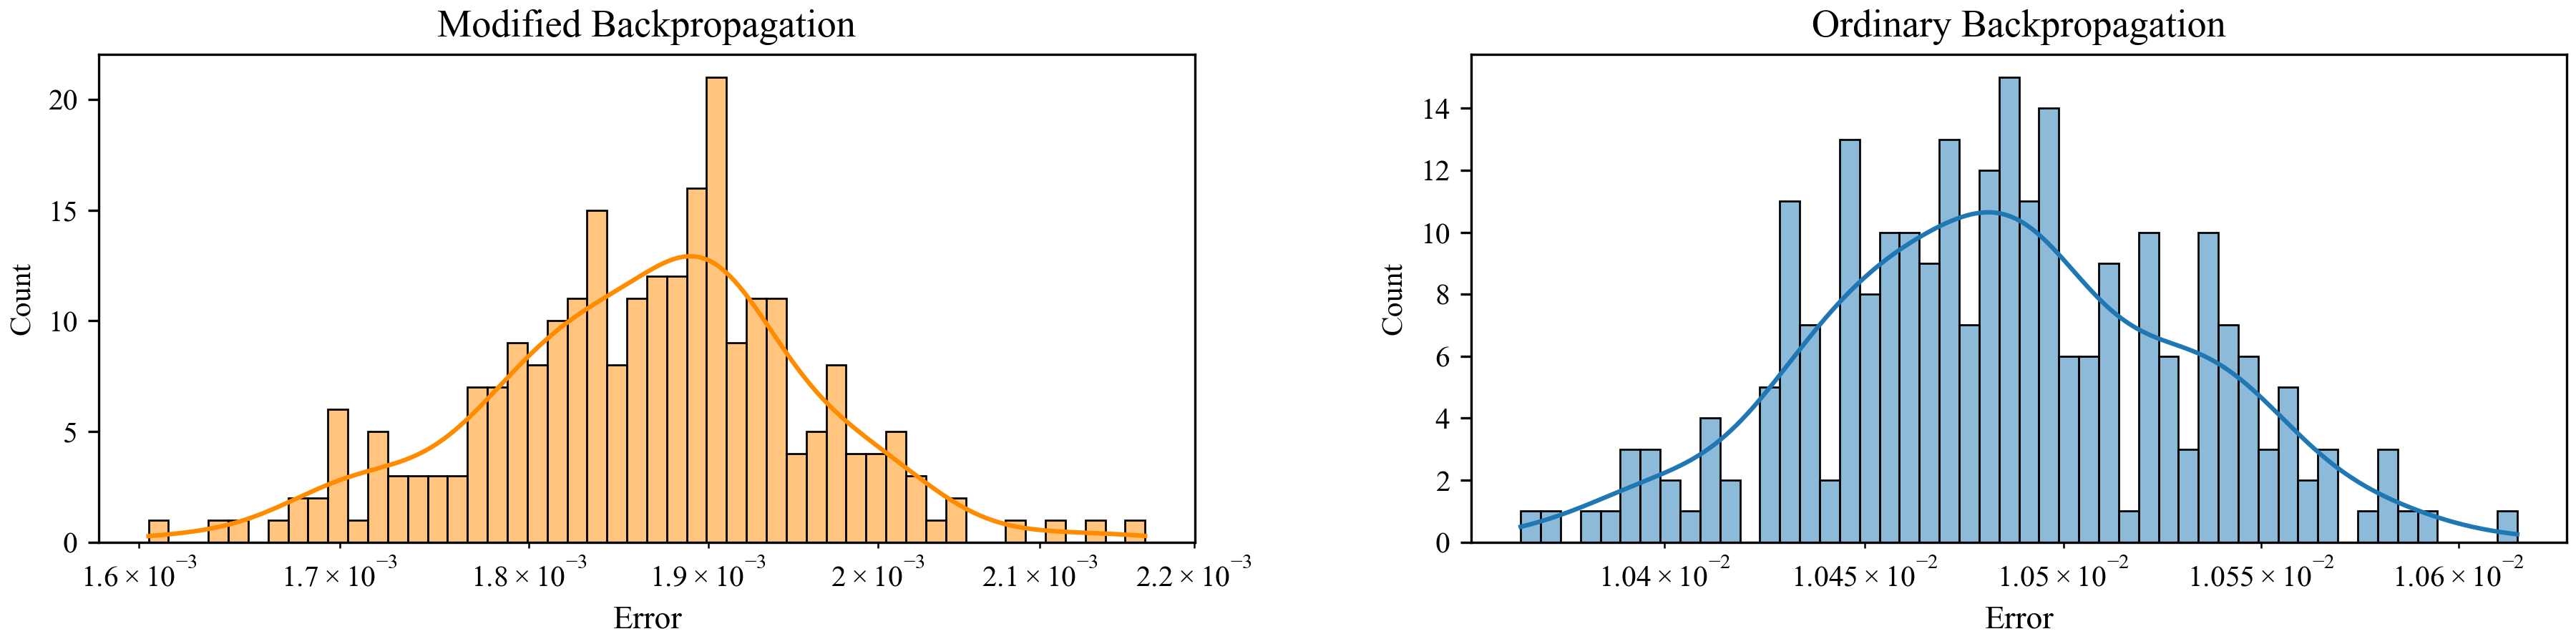
\includegraphics[width=.9\linewidth]{resources/hist_abs_err_b4.png}
    }
    \caption{For each network we report the distribution of \textbf{absolute idempotent error} after 2500 epochs of training 250 randomly initialized networks. Note that distributions are narrow for each algorithm and often separated by more than an order of magnitude.}
    \label{fig:error-test-nets}
\end{figure}

\begin{figure}[H]
    \centering
    \subfigure[Network B1]{
        \label{fig:norm-test-nets-1}
        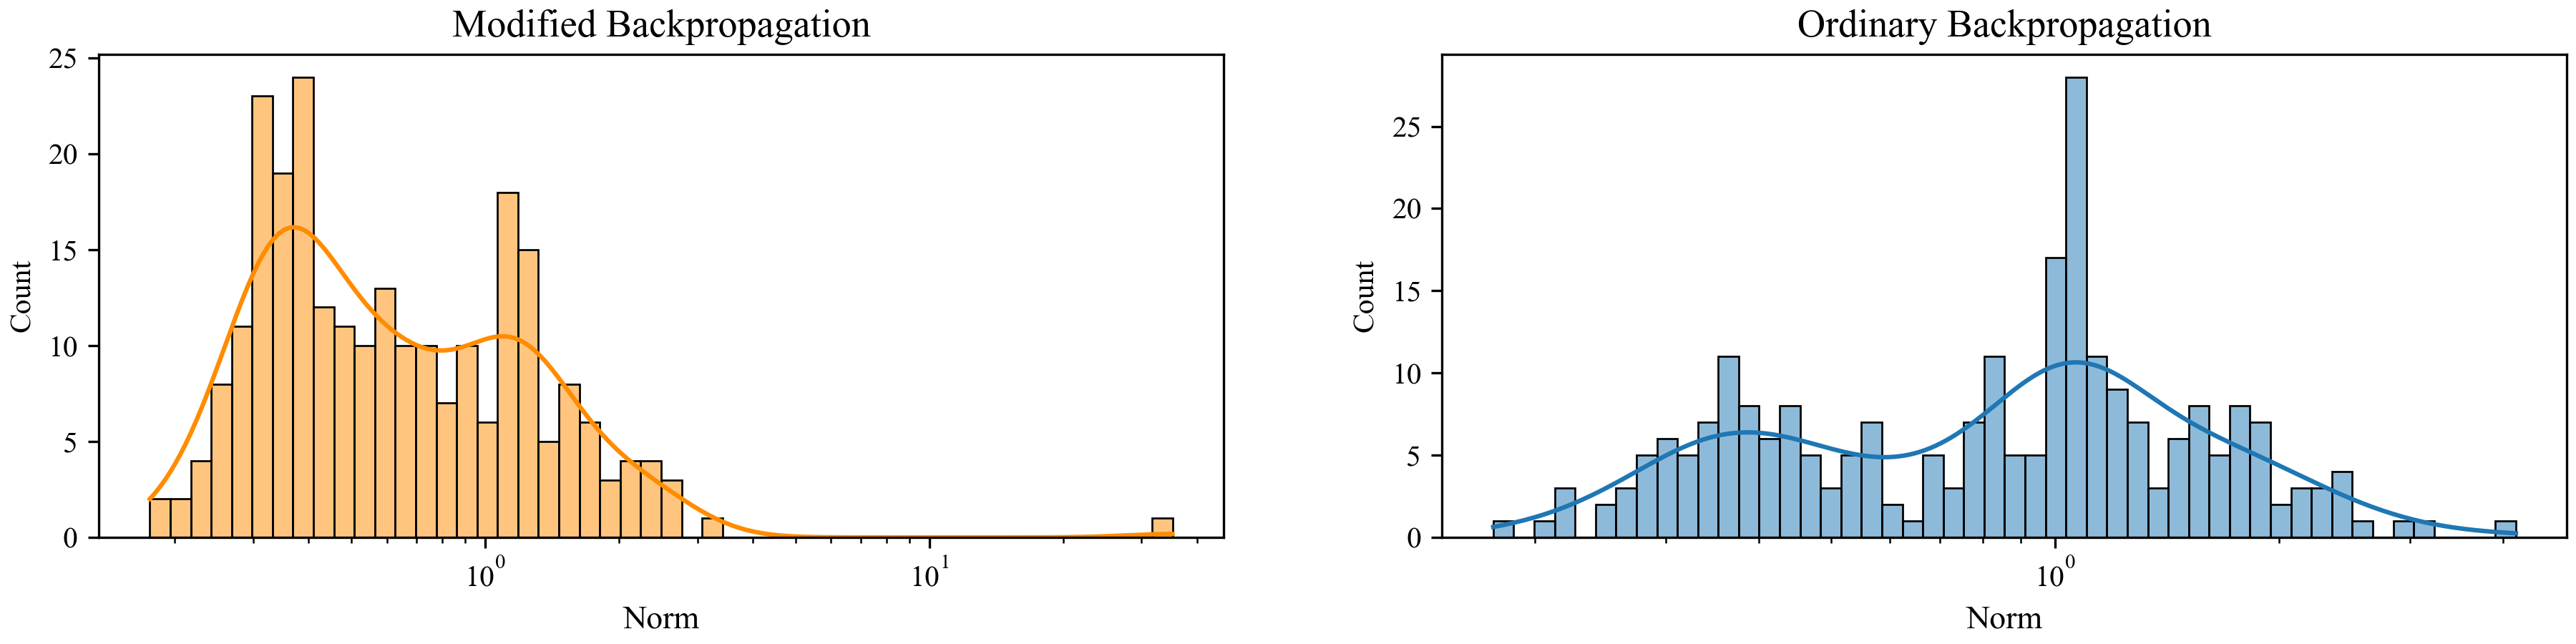
\includegraphics[width=.9\linewidth]{resources/hist-norm-b1.png}
    }
    \subfigure[Network B2]{
        \label{fig:norm-test-nets-2}
        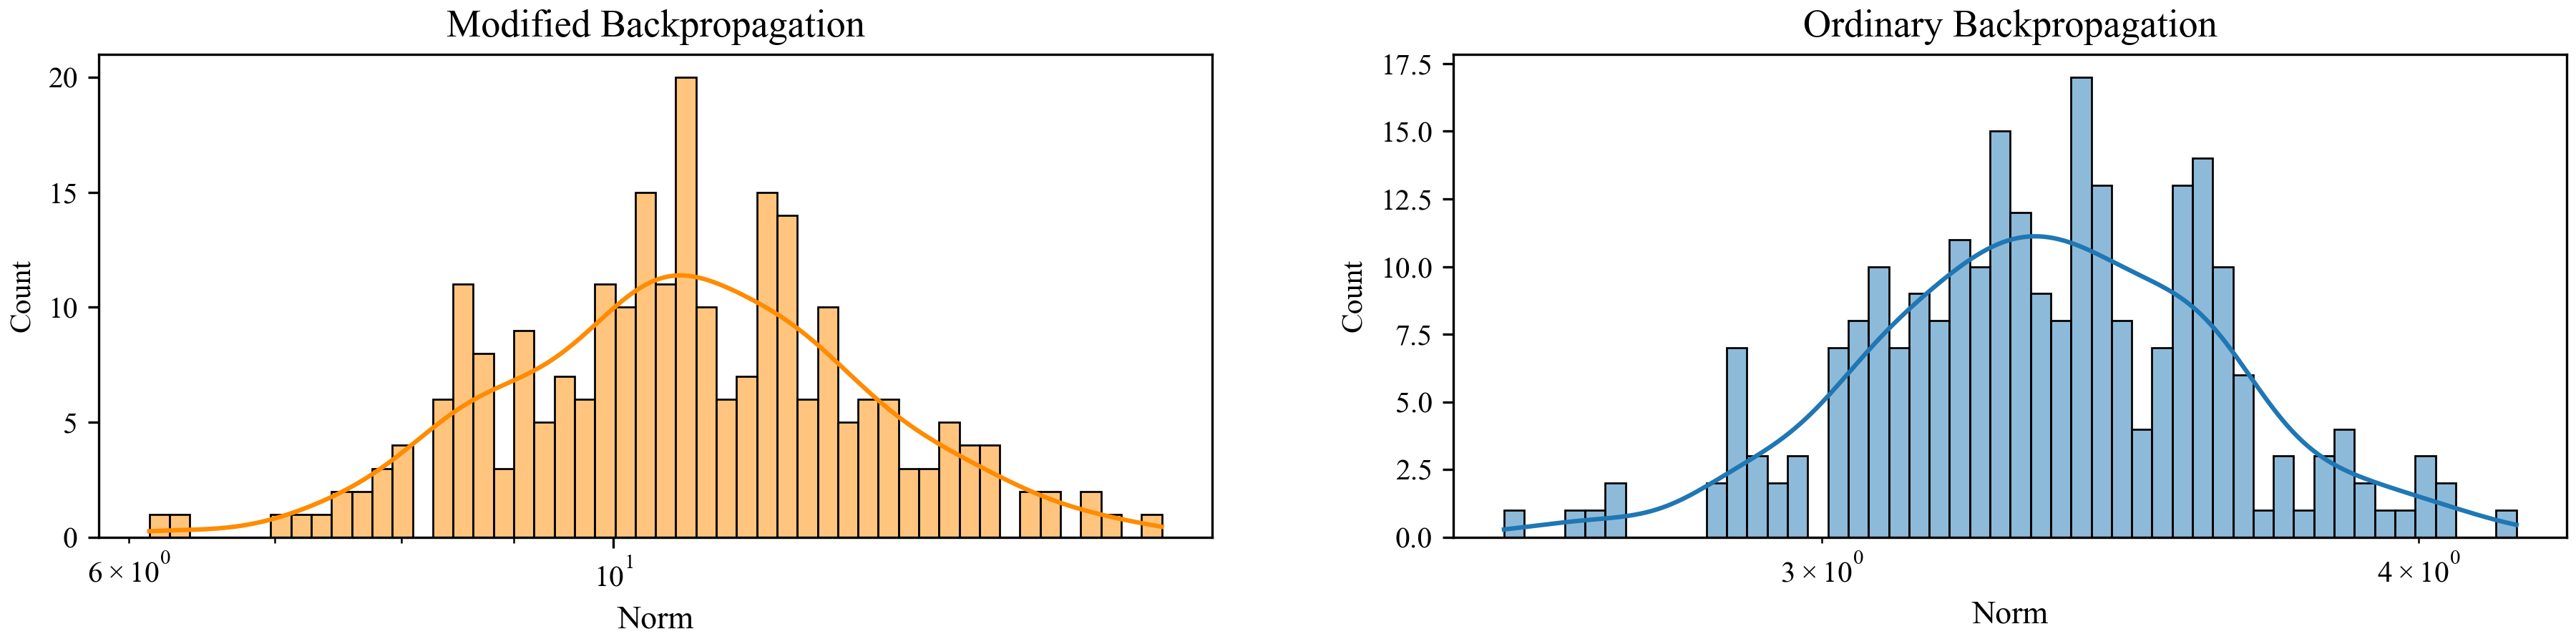
\includegraphics[width=.9\linewidth]{resources/hist-norm-b2.png}
    }
    \subfigure[Network B3]{
        \label{fig:norm-test-nets-3}
        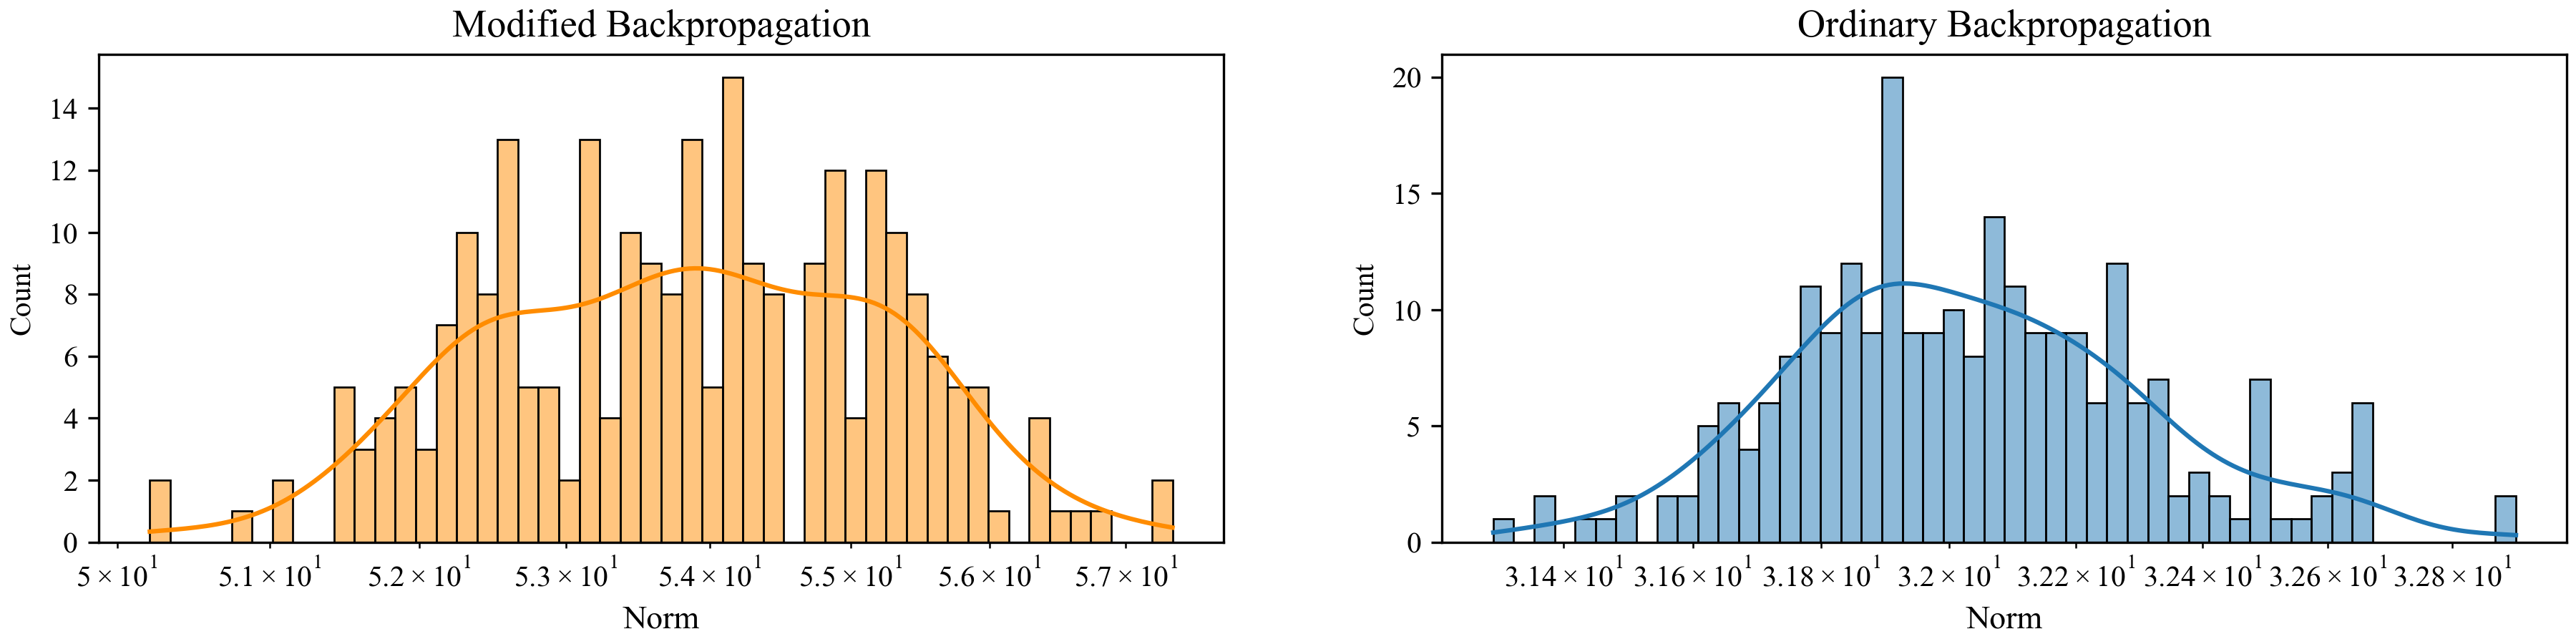
\includegraphics[width=.9\linewidth]{resources/hist-norm-b3.png}
    }
    \subfigure[Network B4]{
        \label{fig:norm-test-nets-4}
        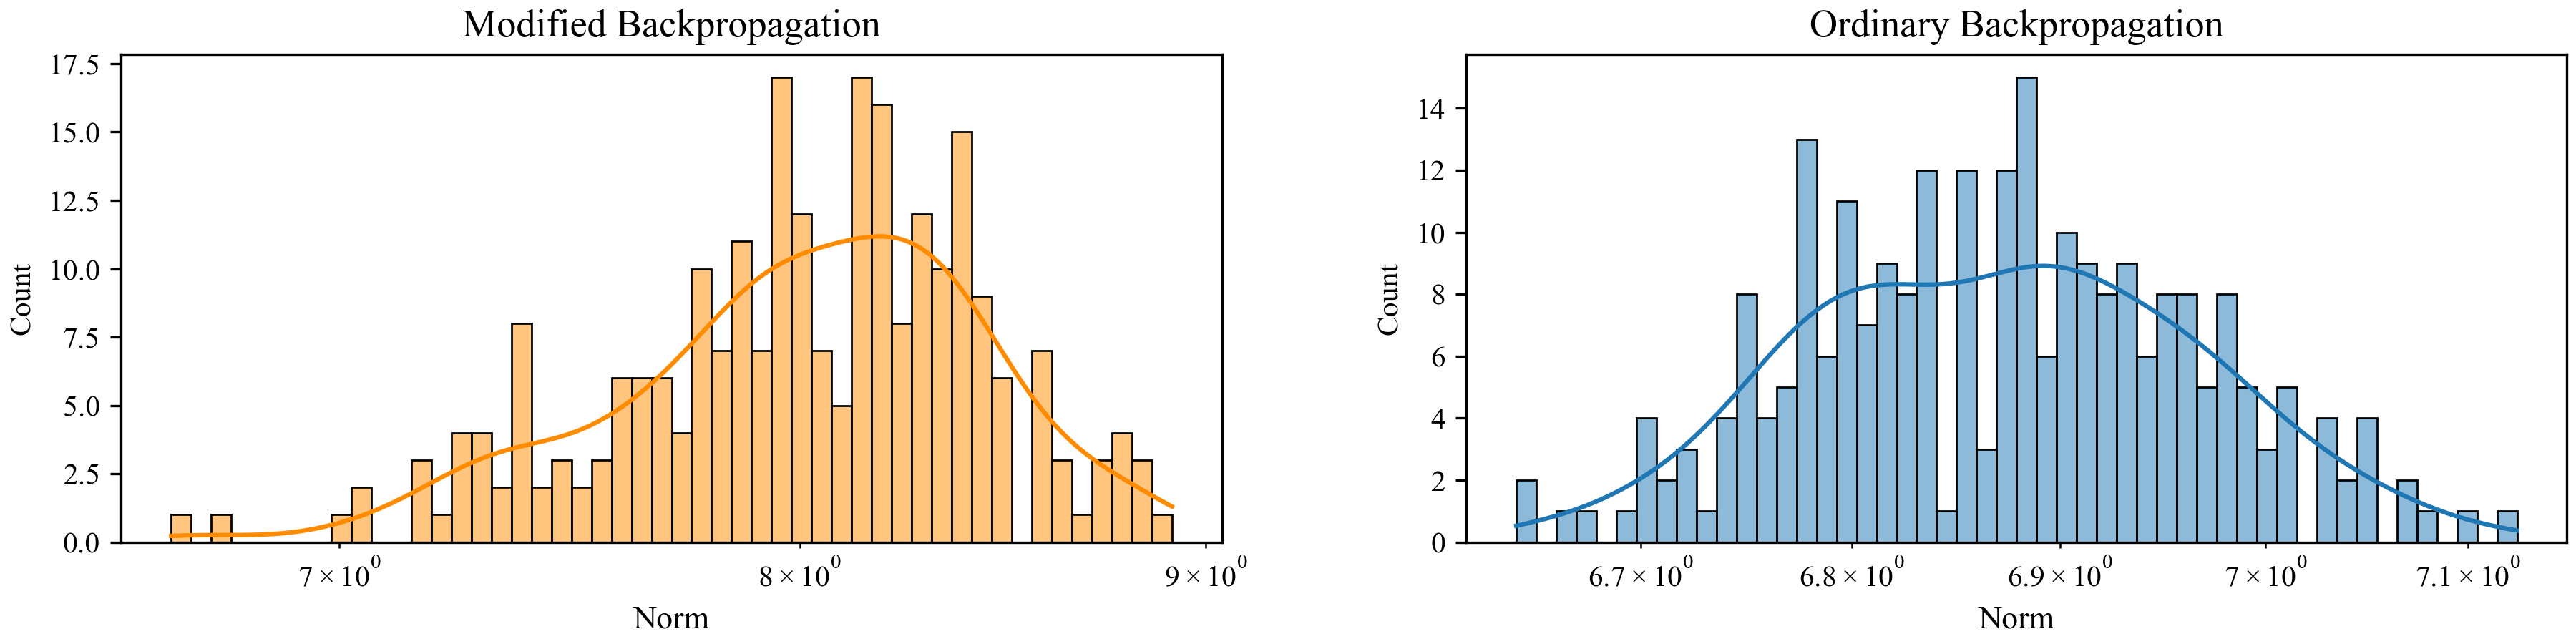
\includegraphics[width=.9\linewidth]{resources/hist-norm-b4.png}
    }
    \caption{For each network we report the distribution of \textbf{norms} after 2500 epochs of training 250 randomly initialized networks. Note that distributions for either method are not centred around zero, indicating that the trained network is a non-trivial idempotent mapping. To calculate the norm we pass each canonical basis vector of $\mathbb{R}^n$ as input by concatenating them into the identity matrix and report here the Frobenius norm of the output matrix.}
    \label{fig:norm-test-nets}
\end{figure}

\newpage
\section{Generative training scheme}
\label{app:gen-training-scheme}
We follow the example of \citealt{shocher-ign} and train a U-Net style DCGAN architecture on the MNIST dataset. Let $\mathcal{L}$ denote the latent space and $\mathcal{X}$ denote the sample space. Then, letting ${G: \mathcal{L} \to \mathcal{X}}$ and ${D: \mathcal{X} \to \mathcal{L}}$ be the Generator and Discriminator of the network respectively, we apply the network $G(D(\vx)) = \vy$.

Table \ref{tab:scheme} explicitly shows the architecture we use, and table \ref{tab:parameters} shows the hyperparameters chosen for training. The core difference between our configuration and that of \citealt{shocher-ign} is the use of dropout layers at some layers.

\begin{table}[htbp]
    \begin{center}
        \begin{tabular}{| c | r c c c c c c l |}
            \hline
                                                                   & \textbf{Layer}  & \textbf{Size} & \textbf{Stride} & \textbf{Padding} & \textbf{Features} & \textbf{Dropout?} & \textbf{BN?} & \textbf{Activation Func} \\
            \hline
            \hline
            \multirow{5}{*}[-0.4ex]{\rotatebox{90}{Discriminator}} & Conv2D          & $4 \times 4$  & $2$             & $1$              & $64$              & \checkmark        & $\times$     & LeakyReLU(0.2)           \\
                                                                   & Conv2D          & $4 \times 4$  & $2$             & $1$              & $128$             & \checkmark        & \checkmark   & LeakyReLU(0.2)           \\
                                                                   & Conv2D          & $3 \times 3$  & $1$             & $0$              & $256$             & \checkmark        & \checkmark   & LeakyReLU(0.2)           \\
                                                                   & Conv2D          & $3 \times 3$  & $1$             & $0$              & $512$             & \checkmark        & \checkmark   & LeakyReLU(0.2)           \\
                                                                   & Conv2D          & $3 \times 3$  & $1$             & $0$              & $512$             & $\times$          & $\times$     & None                     \\
            \hline
            \multirow{5}{*}[-0.4ex]{\rotatebox{90}{Generator}}     & ConvTranspose2D & $3 \times 3$  & $1$             & $0$              & $256$             & \checkmark        & \checkmark   & ReLU                     \\
                                                                   & ConvTranspose2D & $3 \times 3$  & $1$             & $0$              & $128$             & \checkmark        & \checkmark   & ReLU                     \\
                                                                   & ConvTranspose2D & $3 \times 3$  & $1$             & $0$              & $64$              & \checkmark        & \checkmark   & ReLU                     \\
                                                                   & ConvTranspose2D & $4 \times 4$  & $2$             & $1$              & $32$              & \checkmark        & \checkmark   & ReLU                     \\
                                                                   & ConvTranspose2D & $4 \times 4$  & $2$             & $1$              & $1$               & $\times$          & $\times$     & Tanh                     \\
            \hline
        \end{tabular}
        \vspace{5pt}
        \caption{Network architecture.}
        \label{tab:scheme}
    \end{center}
\end{table}

\begin{table}[htbp]
    \begin{center}
        \begin{tabular}{| r | p{0.5\textwidth} |}
            \hline
            \textbf{Parameter}         & \textbf{Value}                                                                                                         \\
            \hline
            \hline
            Reconstruction loss metric & ${L_1 = \Vert \vy^{*} - \vy_{\mathrm{pred}} \Vert_1}$                                                                  \\
            Loss terms weighting       & $\lambda_r = 20$, $\lambda_i = 0.1$, $\lambda_r = 0.1$                                                                 \\
            Optimizer                  & Adam(lr = $1.0 \times 10^{-4}$, $\beta_1 = 0.5$, $\beta_2 = 0.999$)                                                    \\
            Dropout probability        & $0.05$                                                                                                                 \\
            Batch Size                 & $512$                                                                                                                  \\
            Epochs                     & $100$                                                                                                                  \\
            Weight initialization      & Default Kaiming Uniform initialization: ${\mathcal{U}(-\sqrt{k}, \sqrt{k})}$, for ${k = \sqrt{1/n}}$ for $n$ features. \\
            \hline
        \end{tabular}
        \vspace{5pt}
        \caption{Training parameters.}
        \label{tab:parameters}
    \end{center}
\end{table}

\newpage
\section{Generative samples}
\label{app:gen-samples}
\begin{figure}[H]
    \centering
    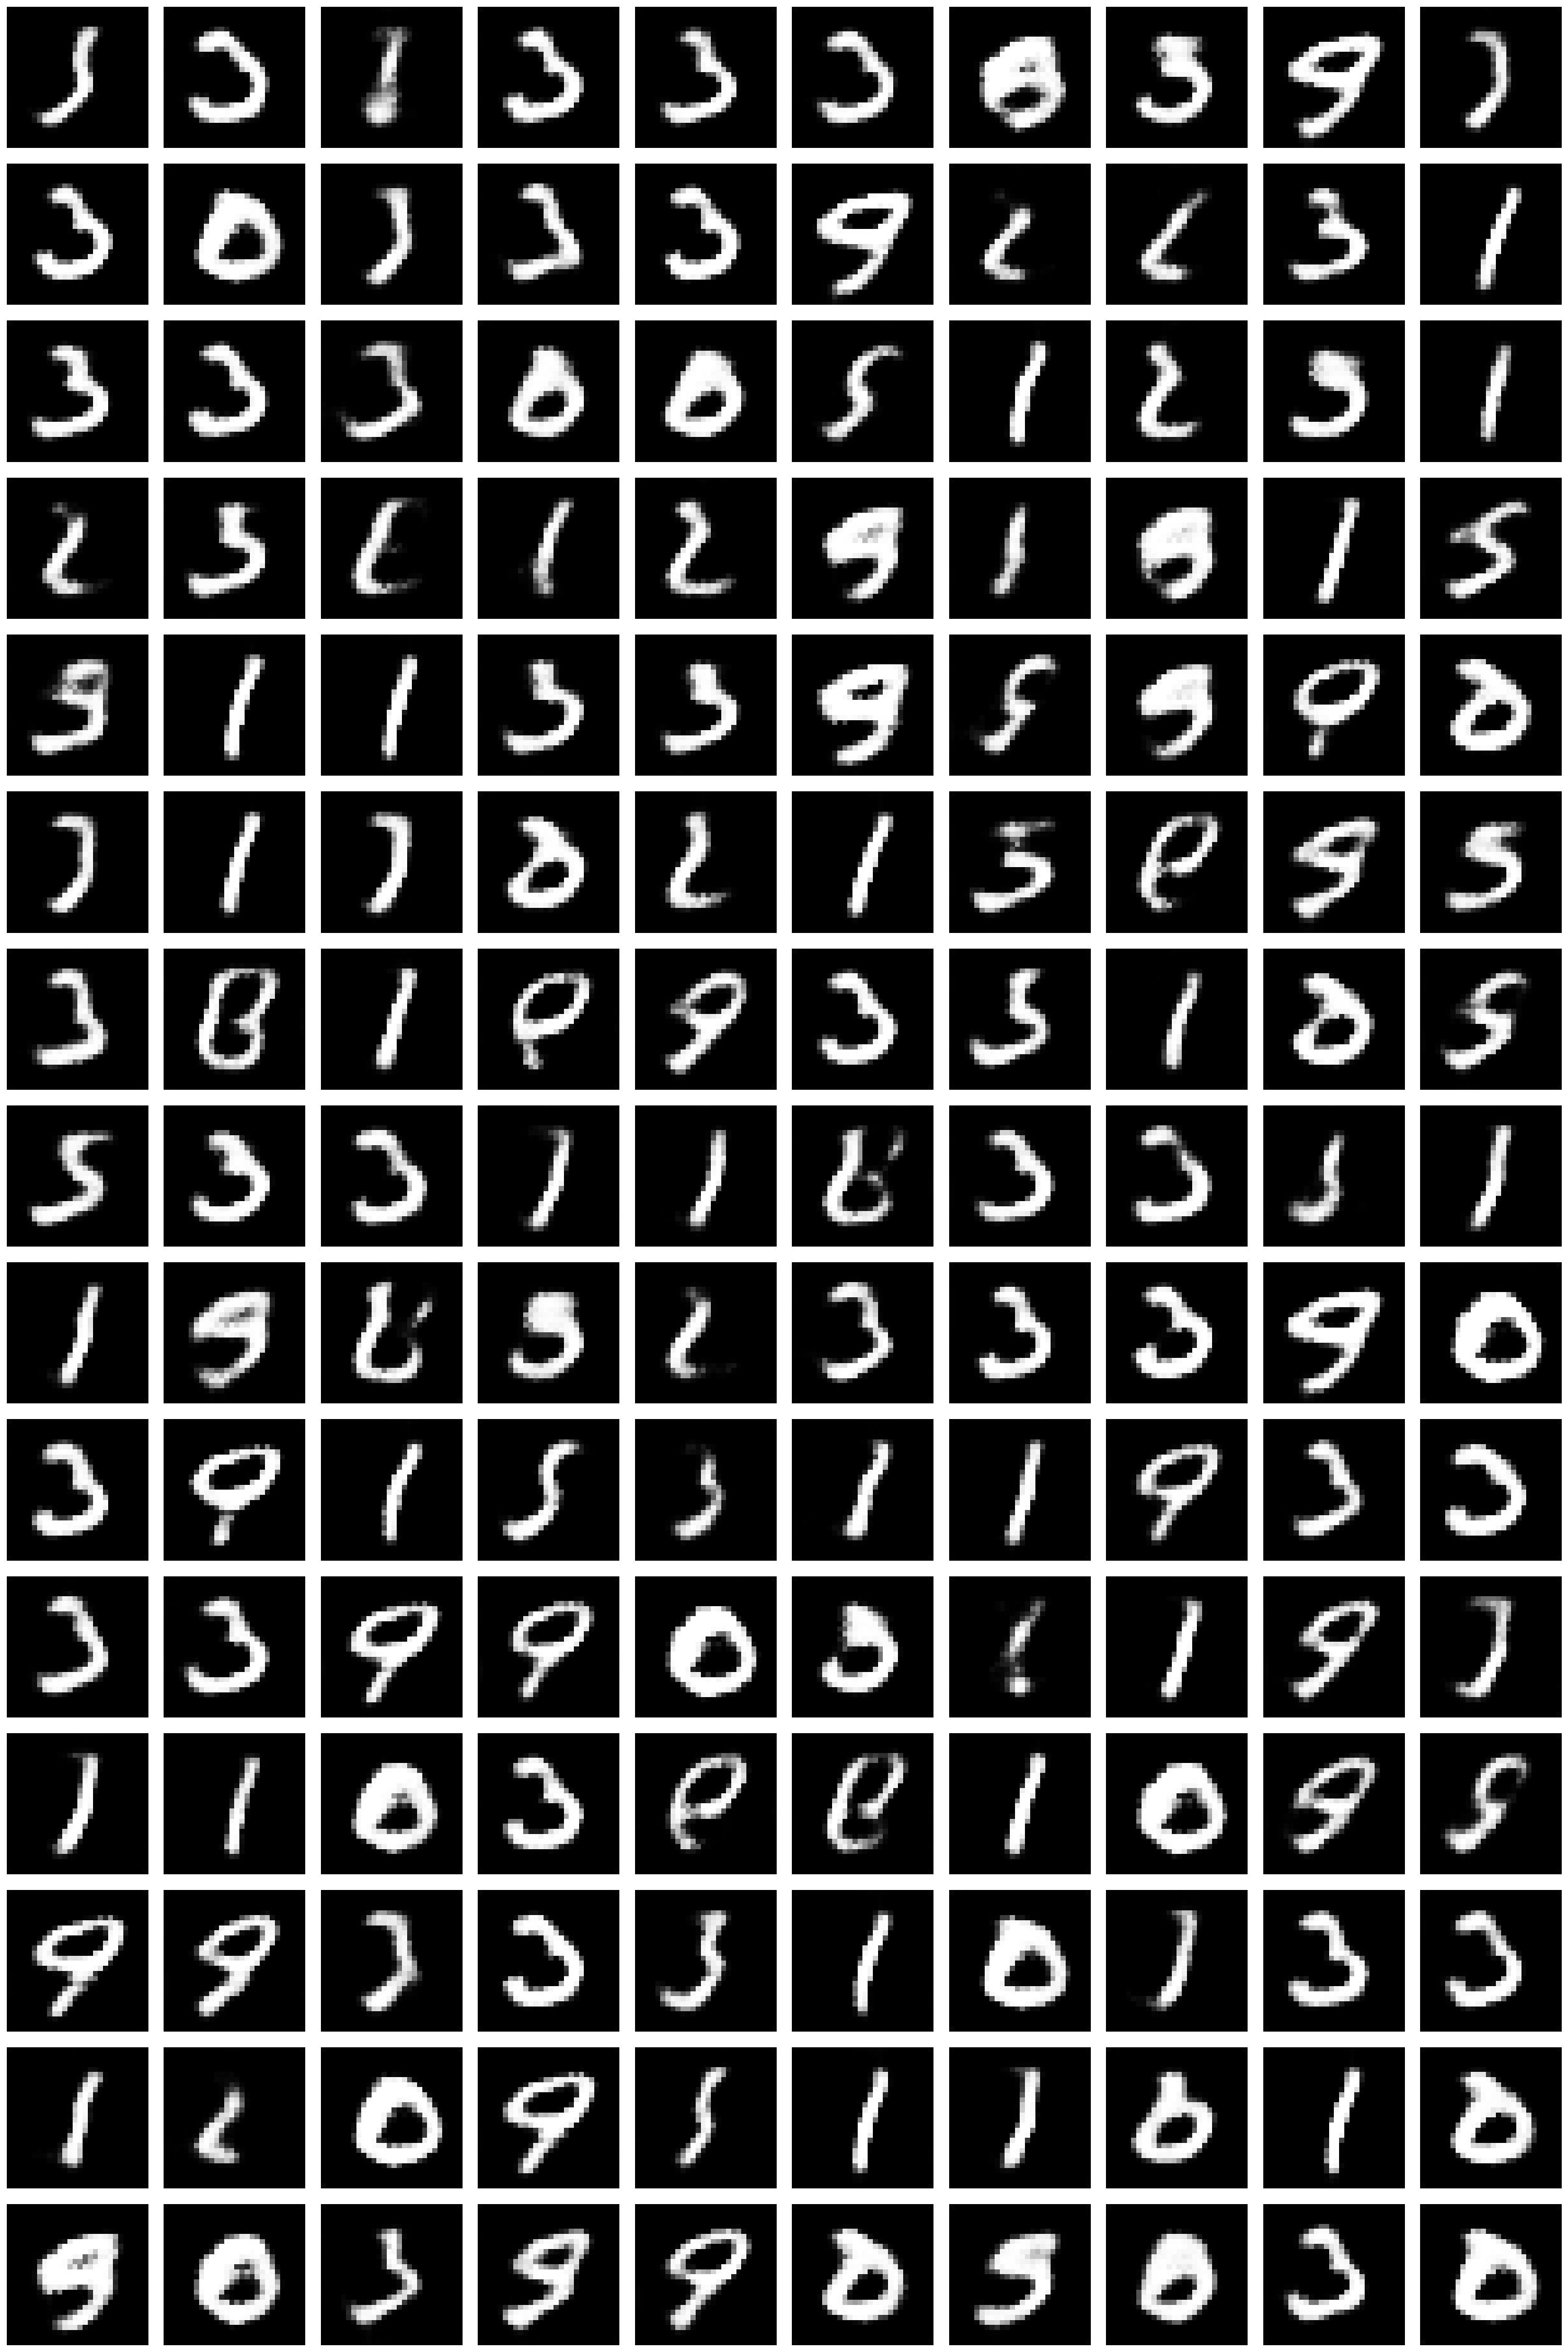
\includegraphics[width=0.65\textwidth]{./resources/modified_0-1_0-1_rand_samples.png}
    \caption{Uncurated generations of U-net style DCGAN model trained on MNIST with Modified Backpropagation for optimizing idempotent and tightness losses. All samples are drawn from a random distribution with mean $0$ and variance $1$, and the result of applying the network is shown.}
    \label{fig:big-gen-mnist}
\end{figure}

\newpage
\section{PCA analysis plots}
% B1 var 90.72
% B2 var 97.81
% B3 var 95.00
% B4 var 98.67
\label{app:pca}
\begin{figure}[H]
    \centering
    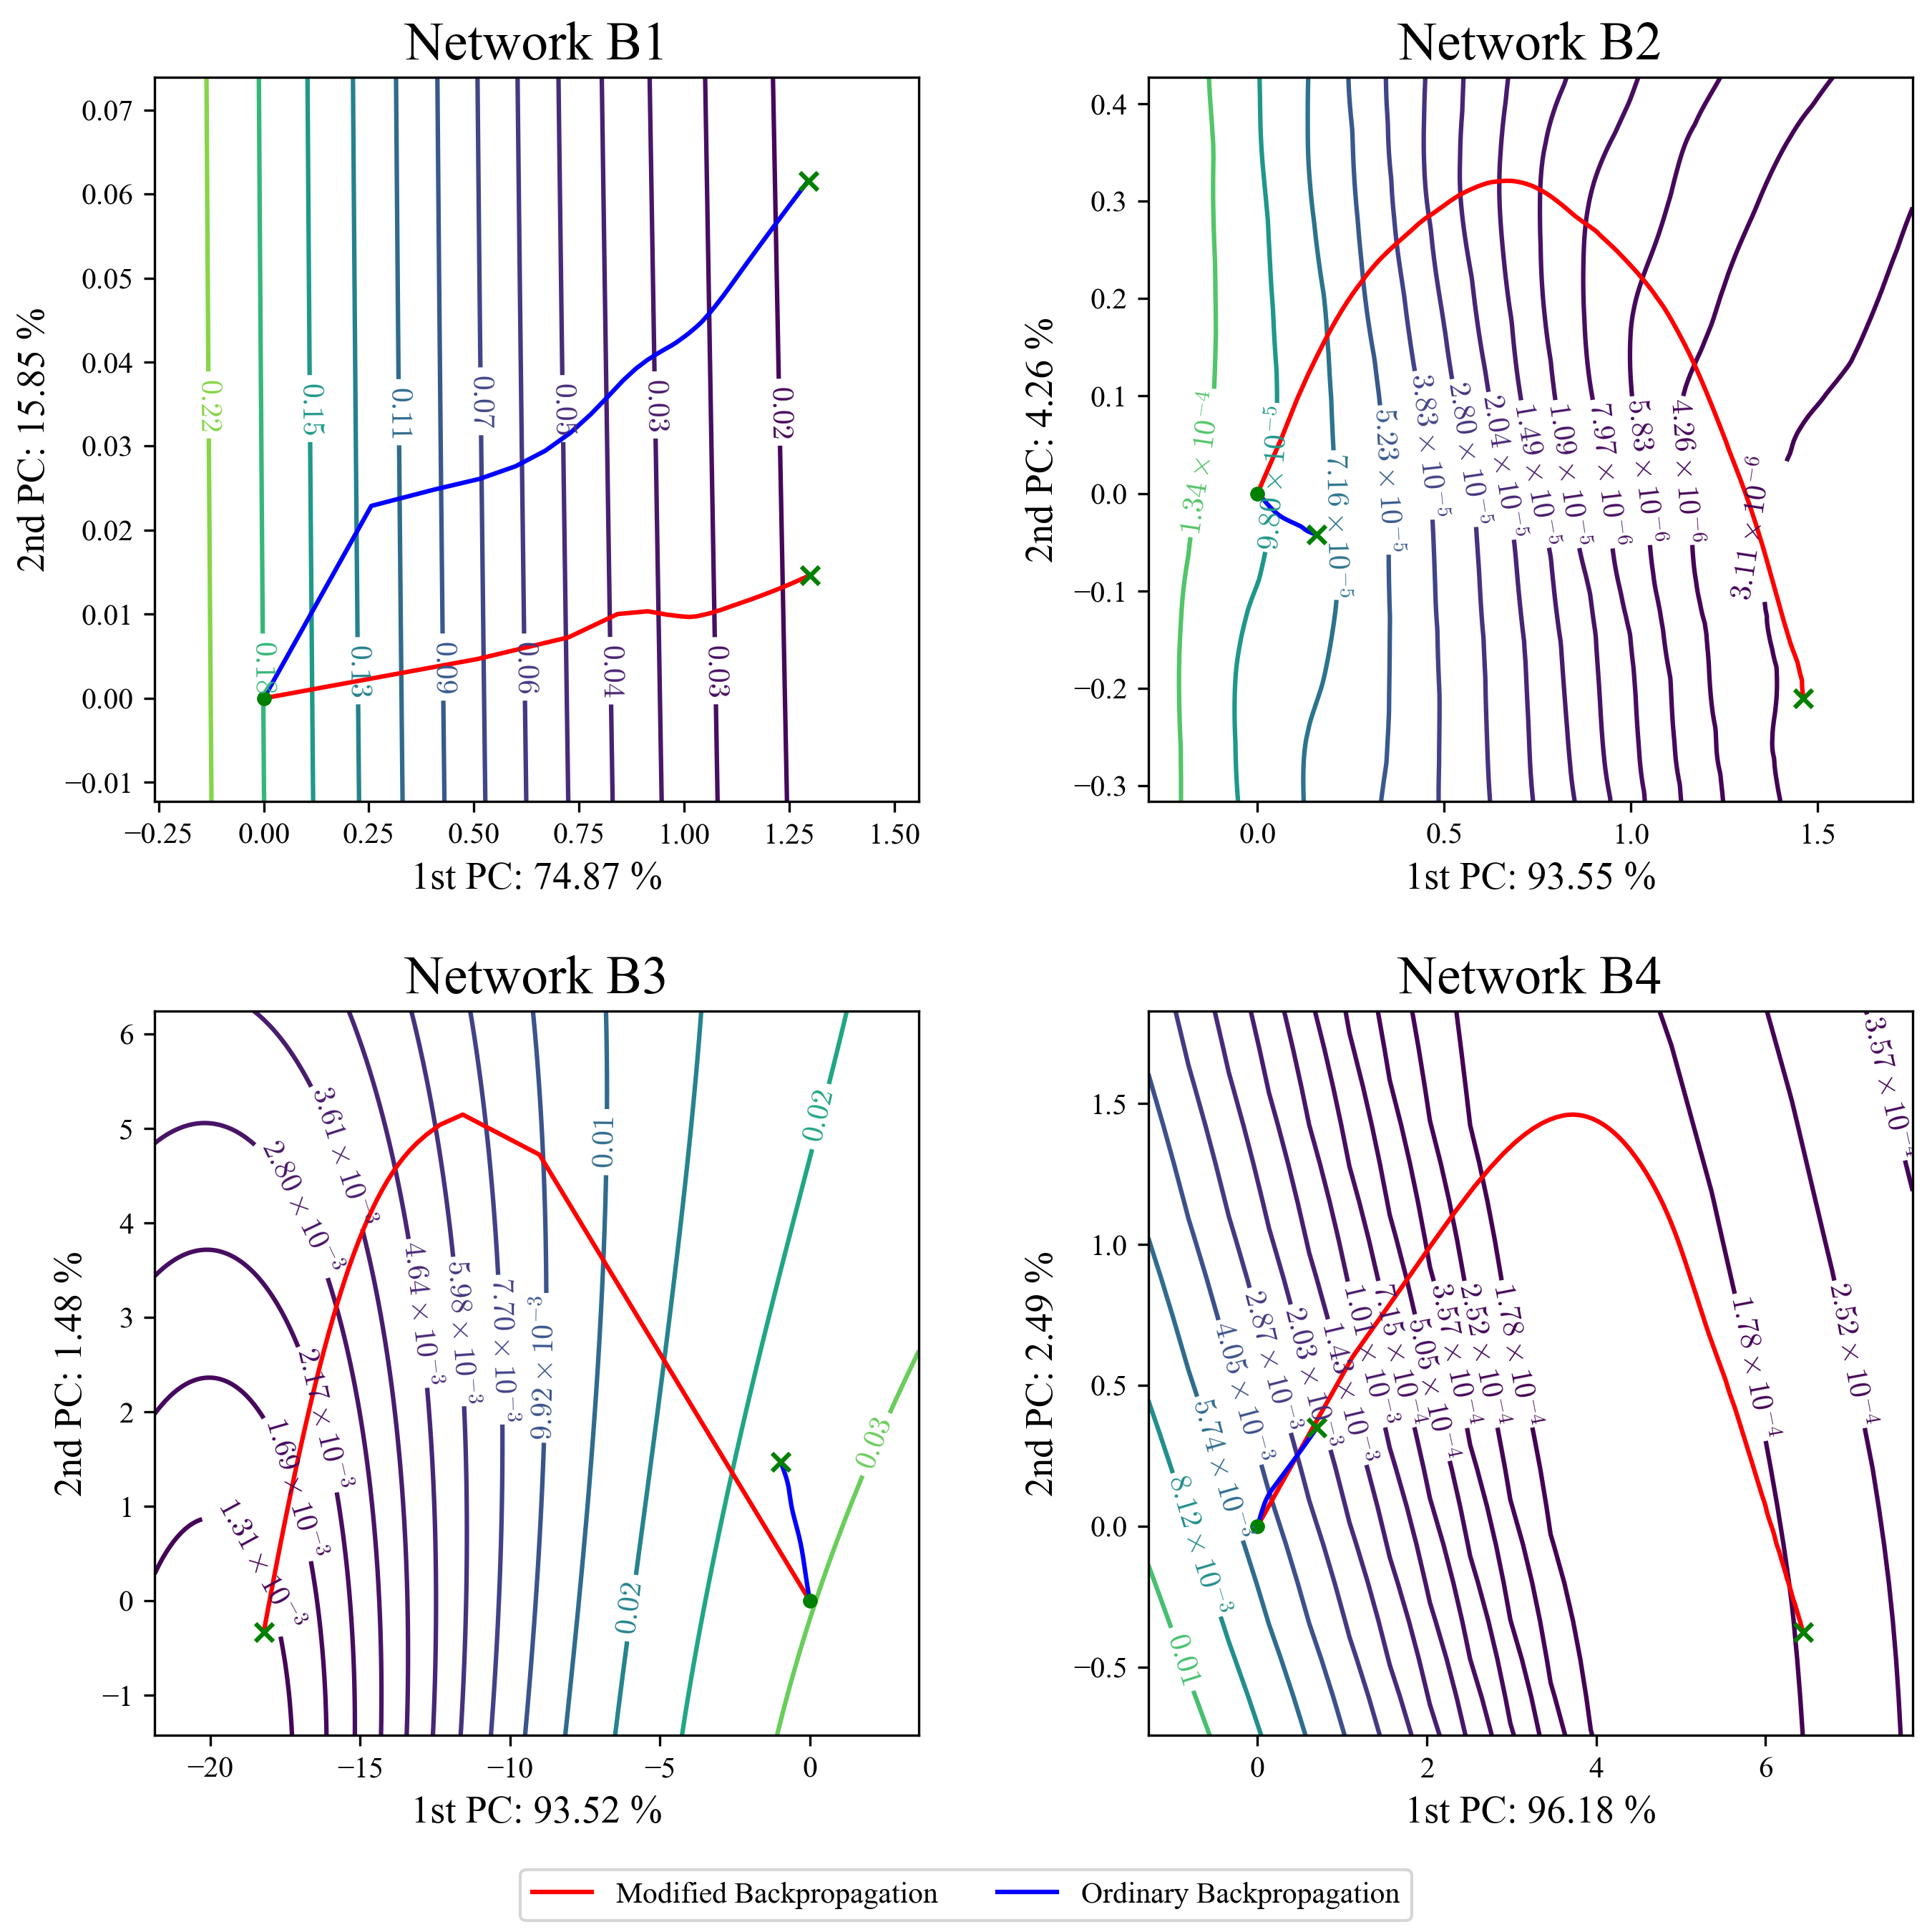
\includegraphics[width=0.8\textwidth]{./resources/pca_all.png}
    \caption{Representative projections of the optimizer trajectories over 2500 epochs of either algorithm on each of the B1-B4 models at optimal learning rates (Figure \ref{fig:avg-abs-err}). Total variance captured is $>90\%$ with cosine similarity of PC1 and PC2 less than $1.0\times10^{-6}$ across all plots. Optimizer trajectory of Modified Backpropagation often deviates significantly from Ordinary Backpropagation, but may sometimes overlap (\textit{e.g.}, B4).}
    \label{fig:big-pca}
\end{figure}

\end{document}


% This document was modified from the file originally made available by
% Pat Langley and Andrea Danyluk for ICML-2K. This version was created
% by Iain Murray in 2018, and modified by Alexandre Bouchard in
% 2019 and 2021 and by Csaba Szepesvari, Gang Niu and Sivan Sabato in 2022.
% Modified again in 2023 and 2024 by Sivan Sabato and Jonathan Scarlett.
% Previous contributors include Dan Roy, Lise Getoor and Tobias
% Scheffer, which was slightly modified from the 2010 version by
% Thorsten Joachims & Johannes Fuernkranz, slightly modified from the
% 2009 version by Kiri Wagstaff and Sam Roweis's 2008 version, which is
% slightly modified from Prasad Tadepalli's 2007 version which is a
% lightly changed version of the previous year's version by Andrew
% Moore, which was in turn edited from those of Kristian Kersting and
% Codrina Lauth. Alex Smola contributed to the algorithmic style files.
